%\documentclass[12pt,compress]{beamer}
%\setbeamertemplate{navigation symbols}{}
\documentclass{beamer}
% This is the file main.tex
%\usetheme{default}
\usetheme{CambridgeUS}
%\usecolortheme{seahorse}
%\usecolortheme{rose}
%\usefonttheme[onlylarge]{structuresmallcapsserif}
%\usefonttheme[onlysmall]{structurebold}
%\setbeamerfont{title}{shape=\itshape,family=\rmfamily}
%\setbeamercolor{title}{fg=red!80!black}
%\setbeamercolor{title}{fg=red!80!black,bg=red!20!white}

% Utilizamos el paquete para usar español
\usepackage[spanish]{babel}
% Utilizamos un paquete para gestionar los acentos
% y las e ¿es
\usepackage[utf8]{inputenc}
% amsmath y amssymb de la American Mathematical 
% Society (fórmulas matemáticas)
\usepackage{amsmath}
\usefonttheme[onlymath]{serif}
%Para que reconozca el entorno verbatim
\usepackage{fancyvrb}
%Definimos nuestra ruta para las imagenes
%Absoluto
%\graphicspath{ {/home/user/images/} }
%Relativo (recomendado) -> según
%https://es.sharelatex.com/learn/Inserting_Images#La_ruta_a_la_carpeta_de_im.C3.A1genes

\usepackage{tikz}
\usepackage{tikz-cd}
\graphicspath{ {media/} }


\title[Mat. Superconductores y sus Aplicaciones]{Detectores de partículas
criogénicos y superconductores}
%Aplicaciones de materiales superconductores en
%								detectores de partículas y radiación}
\vspace{1cm}
\subtitle{{\color[rgb]{0.00,0.21,0.47}Introducción a los materiales
superconductores y sus aplicaciones\\ Instituto Balseiro}}
\author[\texttt{@horacio\_arnaldi}]{L. Horacio Arnaldi}%\\ \texttt{{\href{mailto:arnaldi@cab.cnea.gov.ar}{arnaldi@cab.cnea.gov.ar}}}}
\institute[LabDPR - CAB - IB]{Laboratorio Detección de Partículas y Radiación \\ Centro Atómico Bariloche - Instituto Balseiro}
%\date{\today}
\date{}

\begin{document}

\begin{frame}
				\hspace*{0.6cm}
				
\includegraphics[height=0.18\textheight]{logos/cnea_logo} \hspace*{2.7cm}
				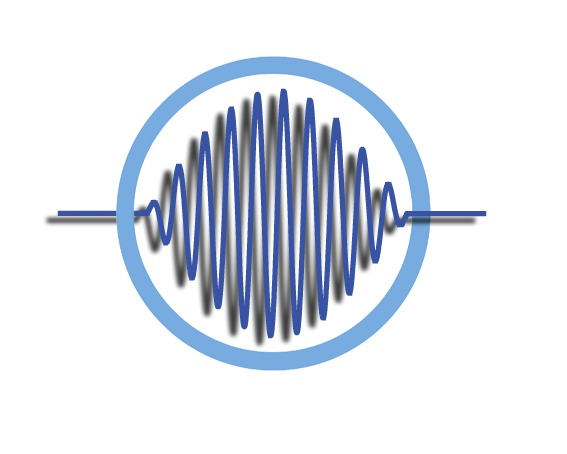
\includegraphics[height=0.18\textheight]{logos/LabDPR_logo} \hspace*{2.7cm}
				
\includegraphics[height=0.18\textheight]{logos/balseiro_logo} %\hspace*{1cm}
				%
\includegraphics[height=0.18\textheight,width=0.15\textwidth]{logos/lagologo}

				\titlepage

\end{frame}

%\begin{frame}
%\frametitle{Contenido}
%\setcounter{tocdepth}{1} %para incluir solo las secciones en el TOC
%\tableofcontents
%%  \tableofcontents[pausesections]
%\end{frame}

%------------------------------------------------------------------------------
\section{Motivación}
%------------------------------------------------------------------------------

\begin{frame}
				\frametitle{Motivación}
				\begin{alertblock}{}
								\alert{¿Por qué usar detectores superconductores cuando ya hay una cantidad de
								detectores para casi cualquier rango de radiación de energía que se
								desee detectar?}
				\end{alertblock}

				\begin{exampleblock}{}
								{\color[rgb]{0.4,0.21,0.68}Proporcionar detectores adecuados
								para algún experimento básico o aplicación que parezca imposible
								sin nuevos detectores}
				\end{exampleblock}
				\begin{exampleblock}{Usar sistemas con mucha menor energía de excitación}
								%\begin{tikzcd}
								\begin{itemize}
												\item detectores gaseosos $\sim$ 20 eV
												\item centelladores líquidos $\sim$ 10 eV
												\item detectores semiconductores $\sim$ 1 eV
												\item \alert{detectores superconductores $\leq$ 10 meV}
								\end{itemize}
								%\end{tikzcd}
				\end{exampleblock}
\end{frame}

\begin{frame}
				\frametitle{Comparación de resoluciones espacial, en tiempo y en energía
				de algunos detectores de radiación}
								\begin{center}
												\begin{tikzpicture}
																\node[anchor=south west,inner sep=0] at (0,0) {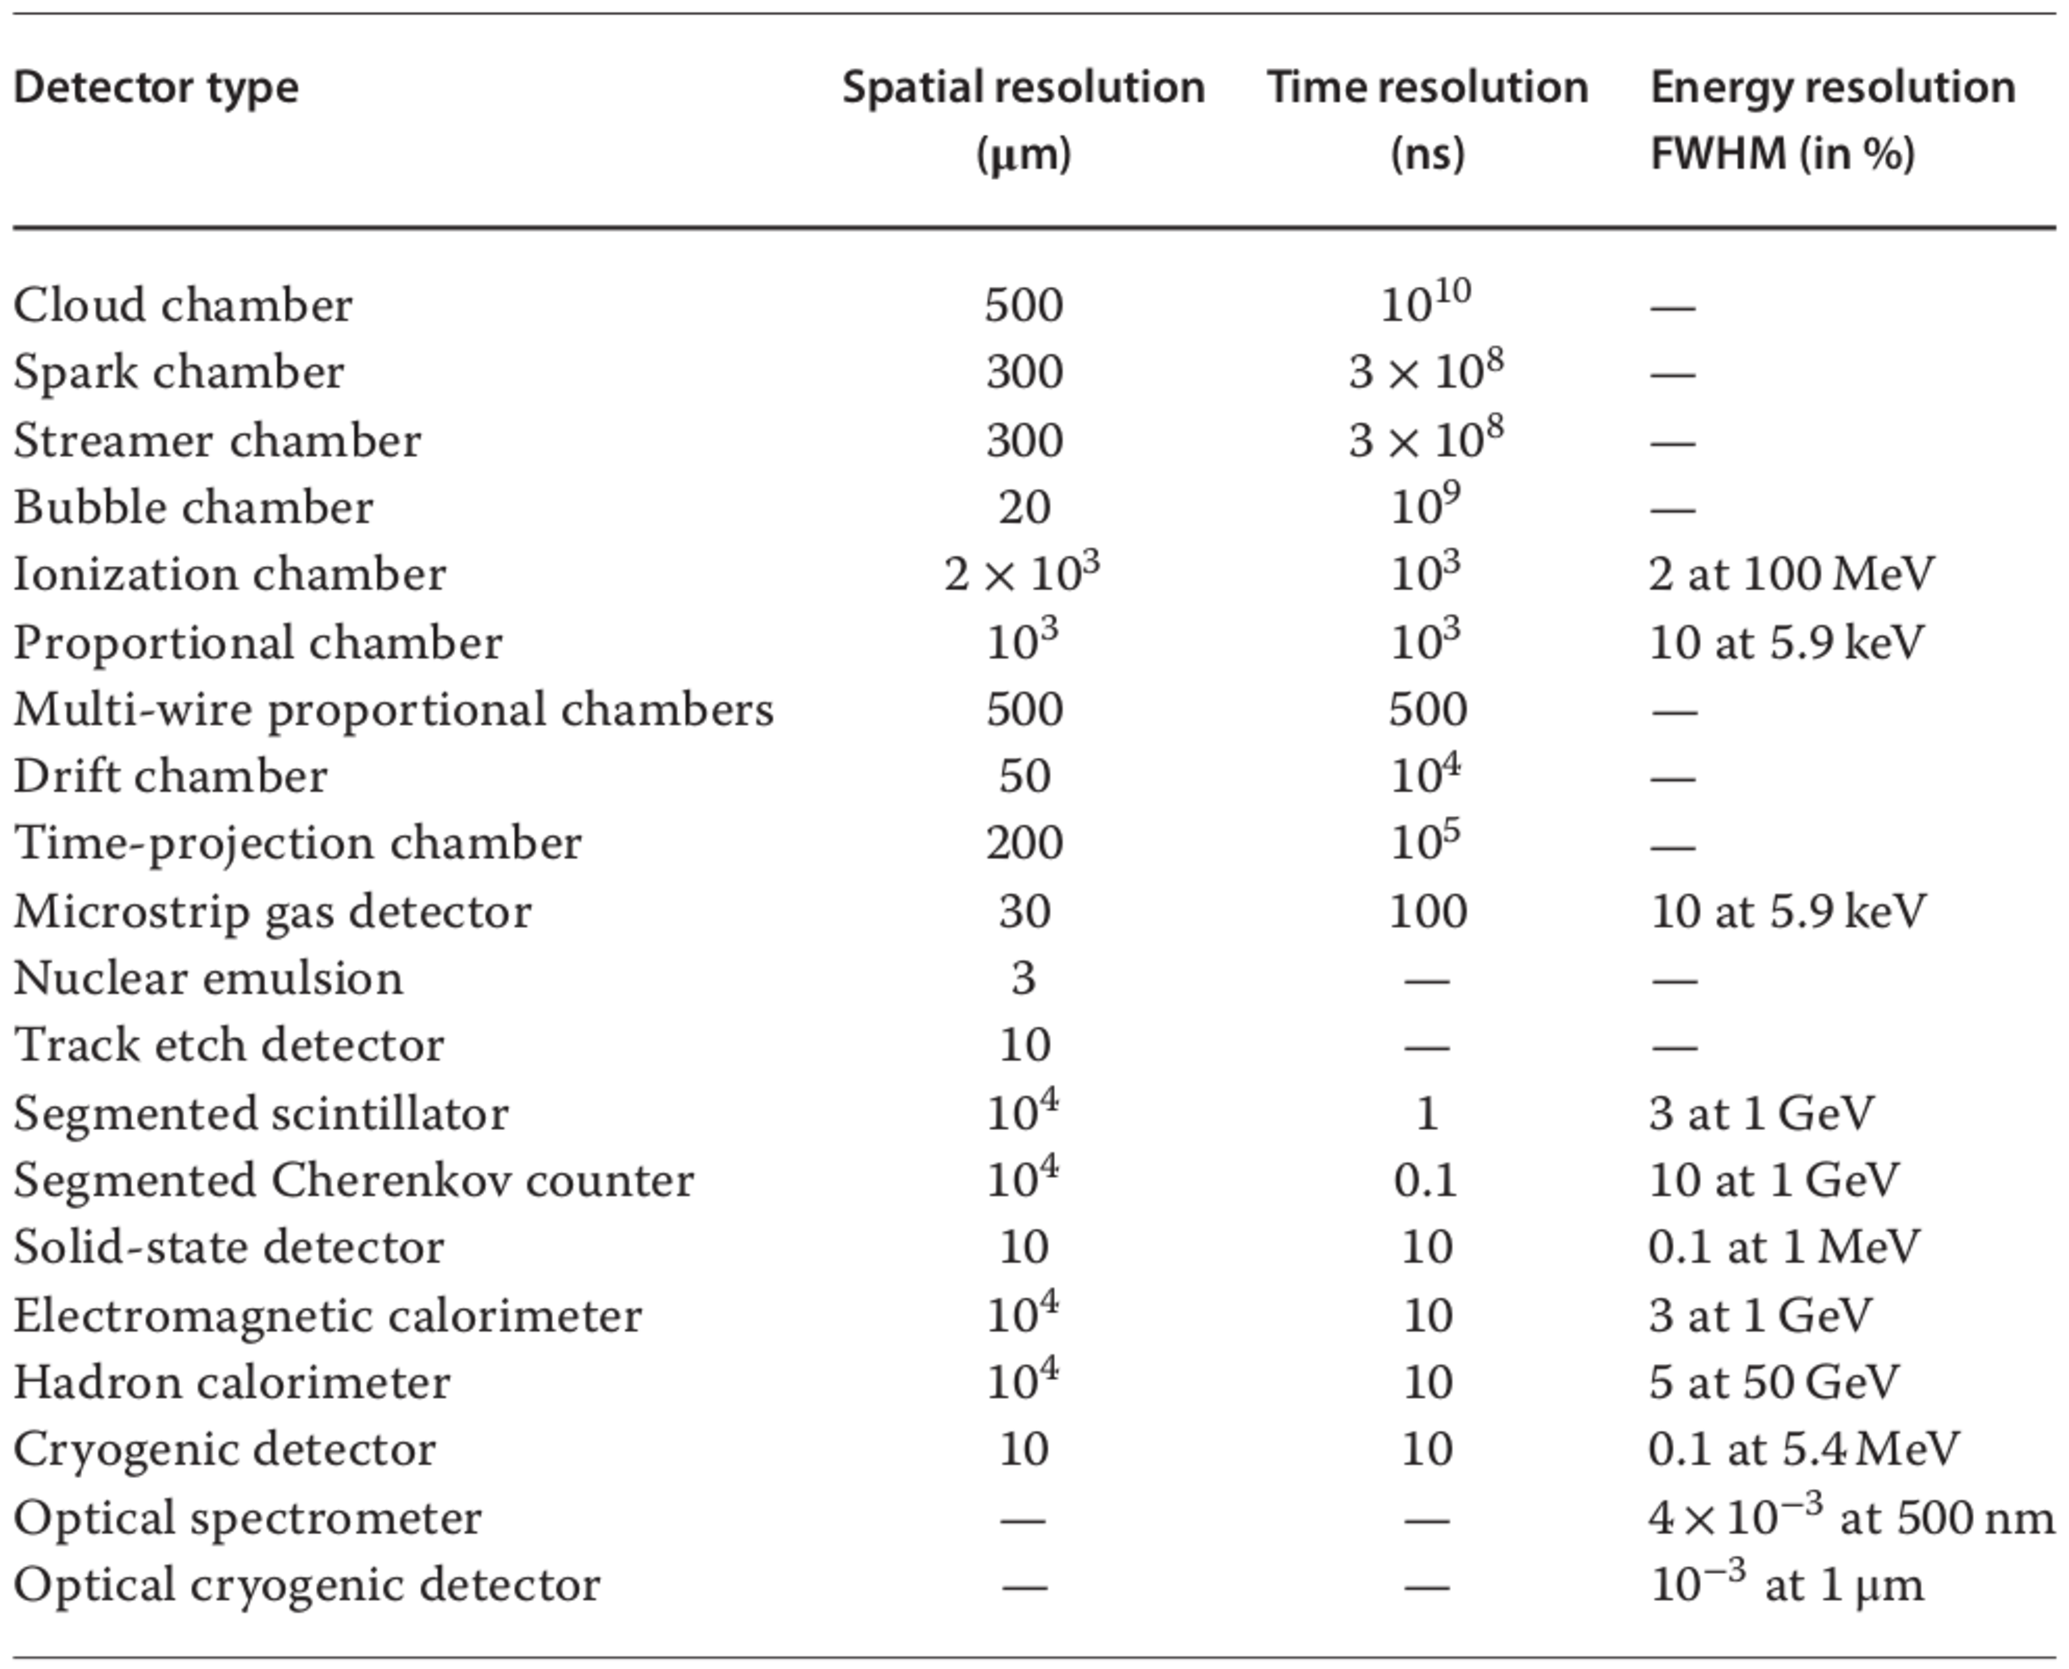
\includegraphics[height=0.68\textheight,width=0.9\textwidth]{tabla_tipos_detectores}};
																\draw<1>[red,ultra thick,rounded corners] (0,.65) rectangle (11,0.95);
																\draw<2>[red,ultra thick,rounded corners] (0,0.18) rectangle (11,.45);
												\end{tikzpicture}
								\end{center}
\end{frame} 

\begin{frame}
				\frametitle{Detección (partículas/radiación)}
				Transferencia de parte o toda la radiación a la masa del detector, donde se convierte en alguna otra forma más accesible a la percepción humana.
								\begin{center}
												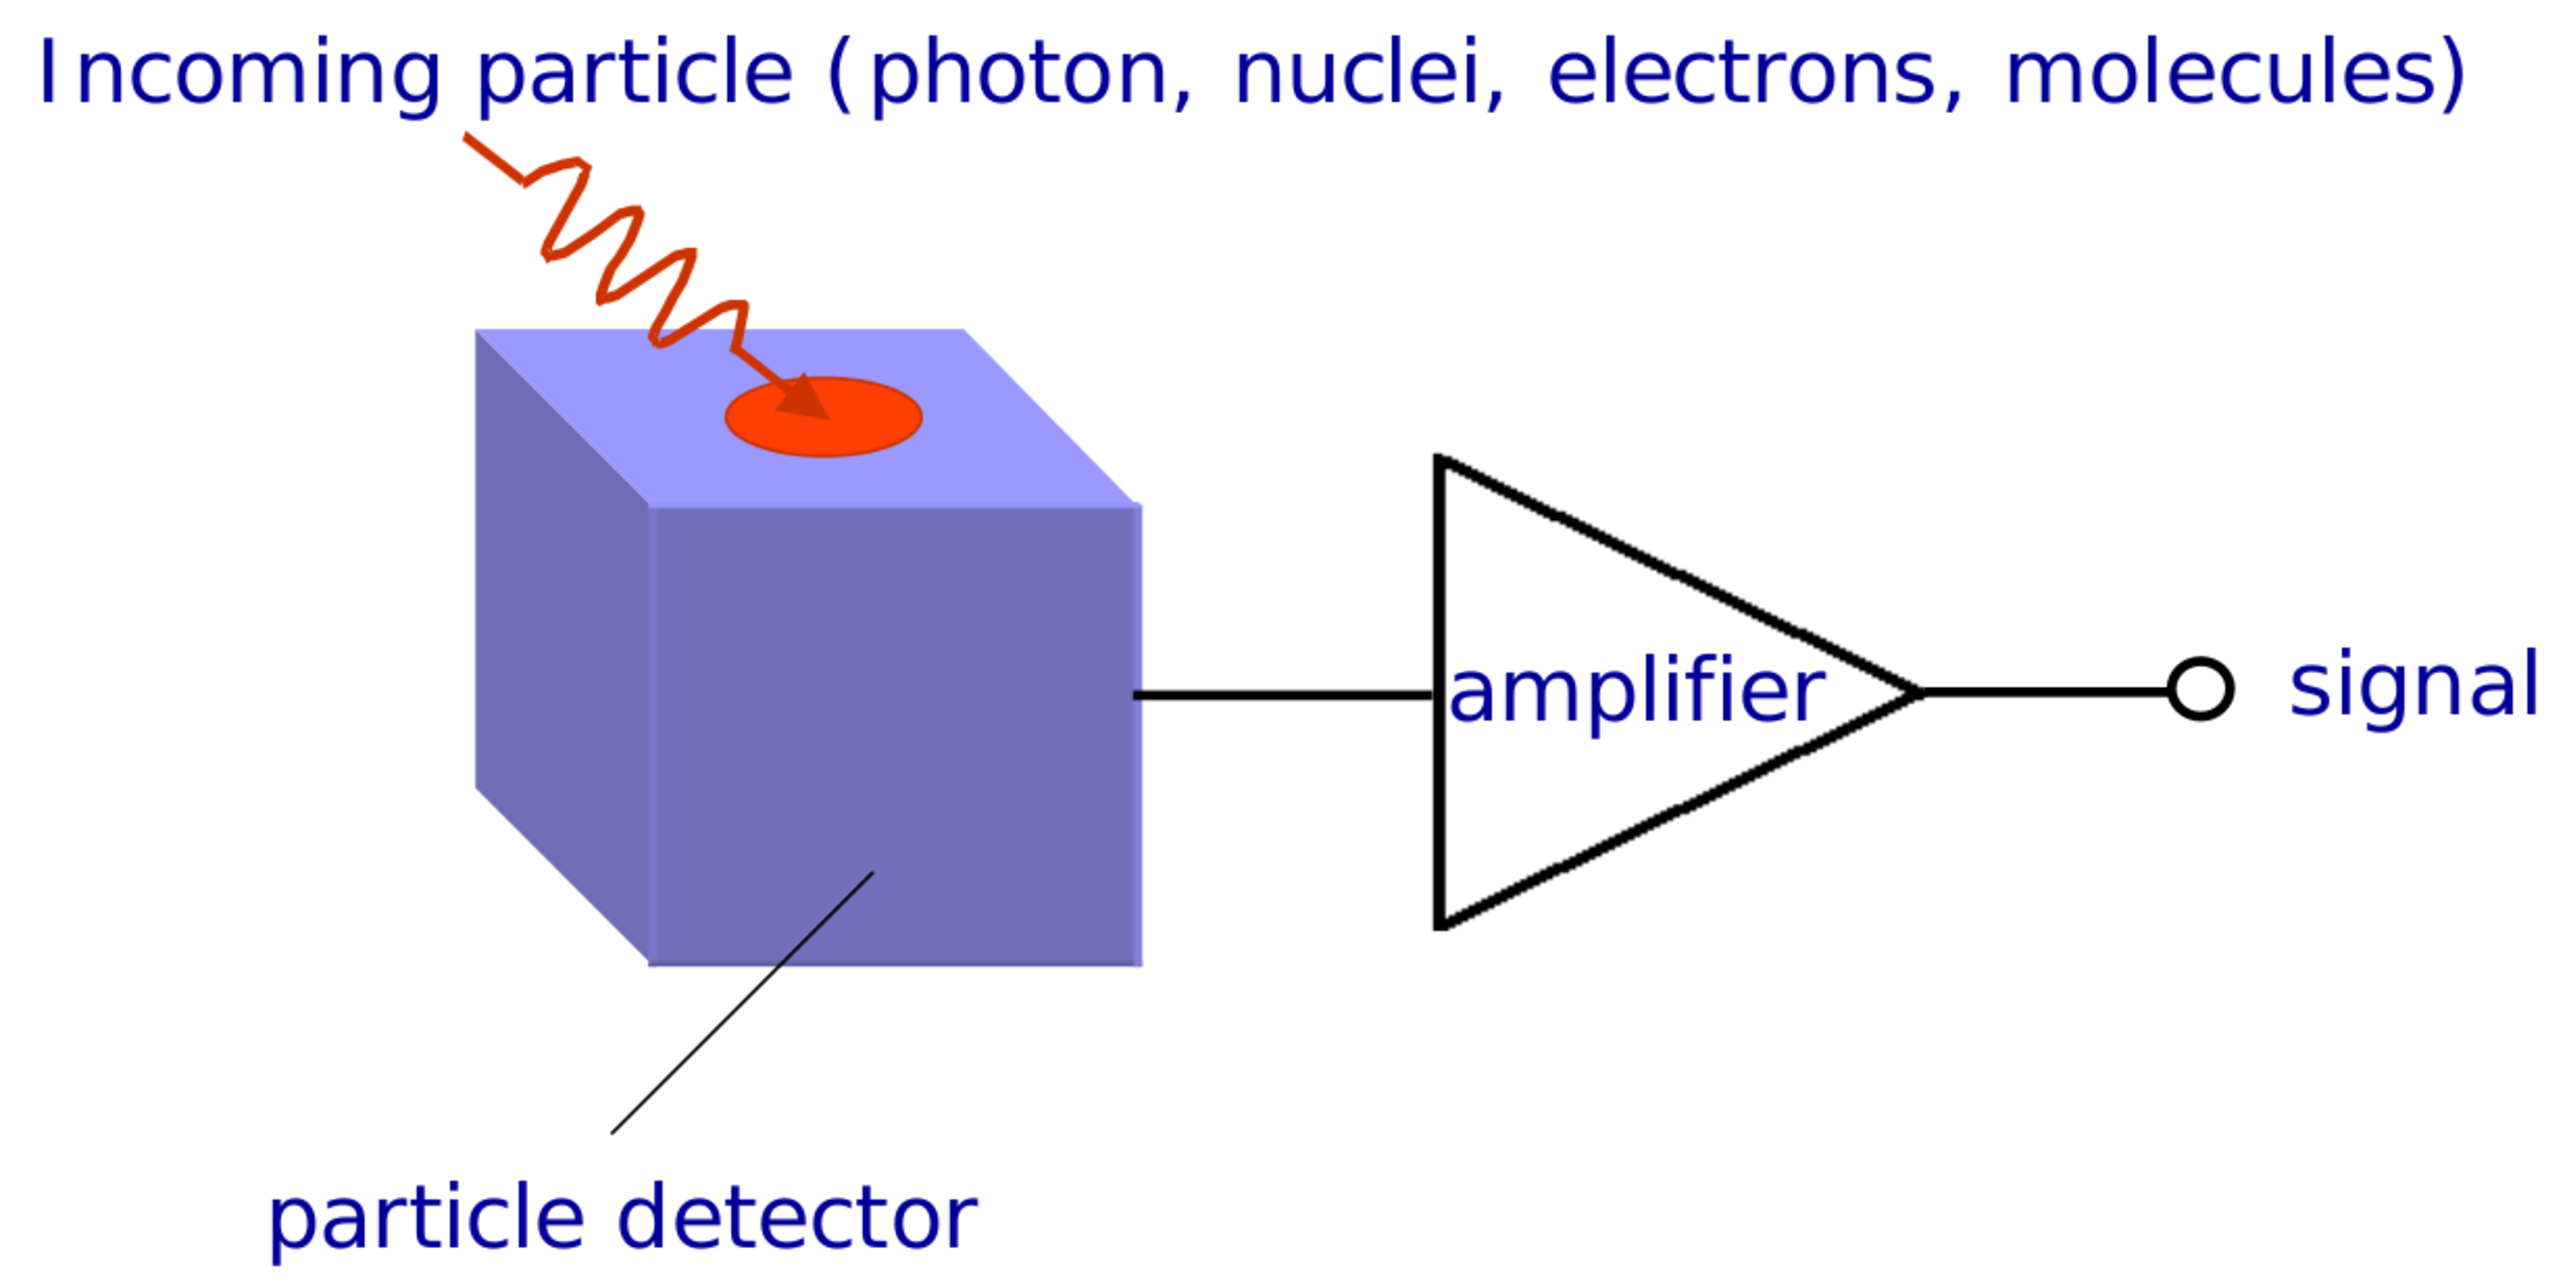
\includegraphics[height=0.4\textheight,width=0.6\textwidth]{deteccion_principio}
								\end{center}
								\begin{itemize}
												\item Ionización
												\item Radiación EM
												\item Partículas neutras $\to$ detección indirecta 
								\end{itemize}
\end{frame}

\begin{frame}
				\frametitle{Detección (partículas/radiación)}
				Transferencia de parte o toda la radiación a la masa del detector, donde se convierte en alguna otra forma más accesible a la percepción humana.
								\begin{center}
												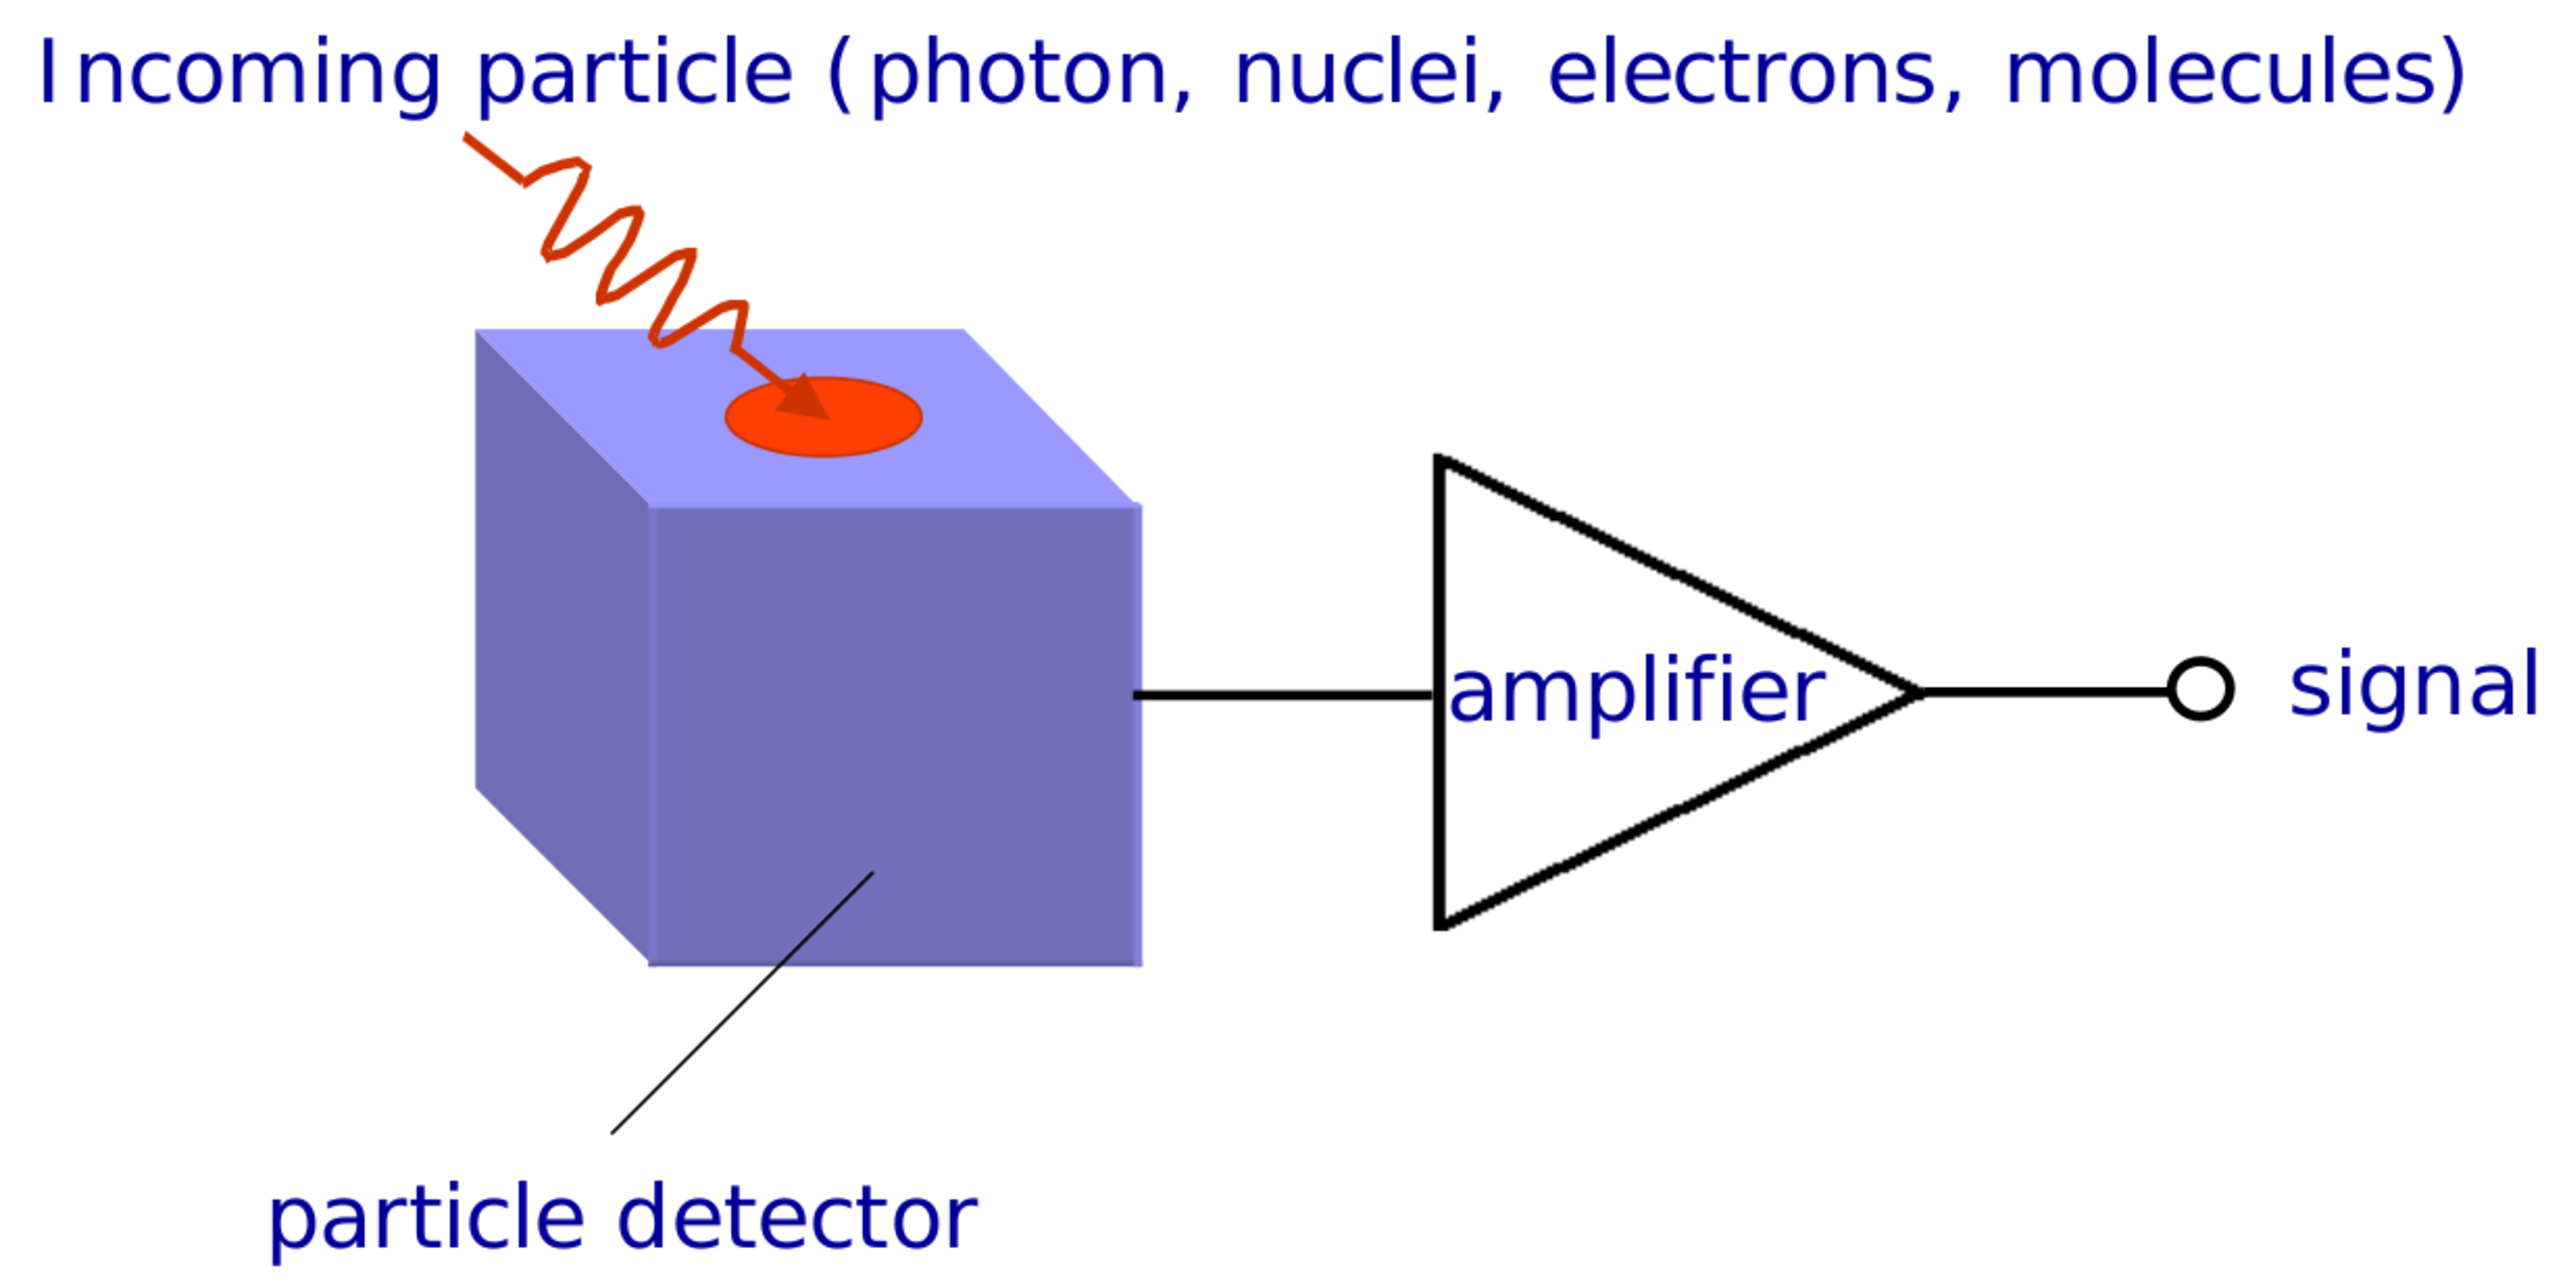
\includegraphics[height=0.4\textheight,width=0.6\textwidth]{deteccion_principio}
								\end{center}
								La pérdida de energía por ionización para partículas
								cargadas (MIP) en la materia se puede
								estimar aproximadamente en \alert{$2\,\text{MeV}$ por
								$\text{g/cm}^2$}.
\end{frame}

\begin{frame}
				\frametitle{Factores de calidad del detector}
				%\begin{exampleblock}{}
								\begin{itemize}
																%								\pause
												\item[*] \alert{Resolución energética $\Delta E/E$:}
																Capacidad de distinguir dos energías cercanas
																\begin{center}
																				\only<1>{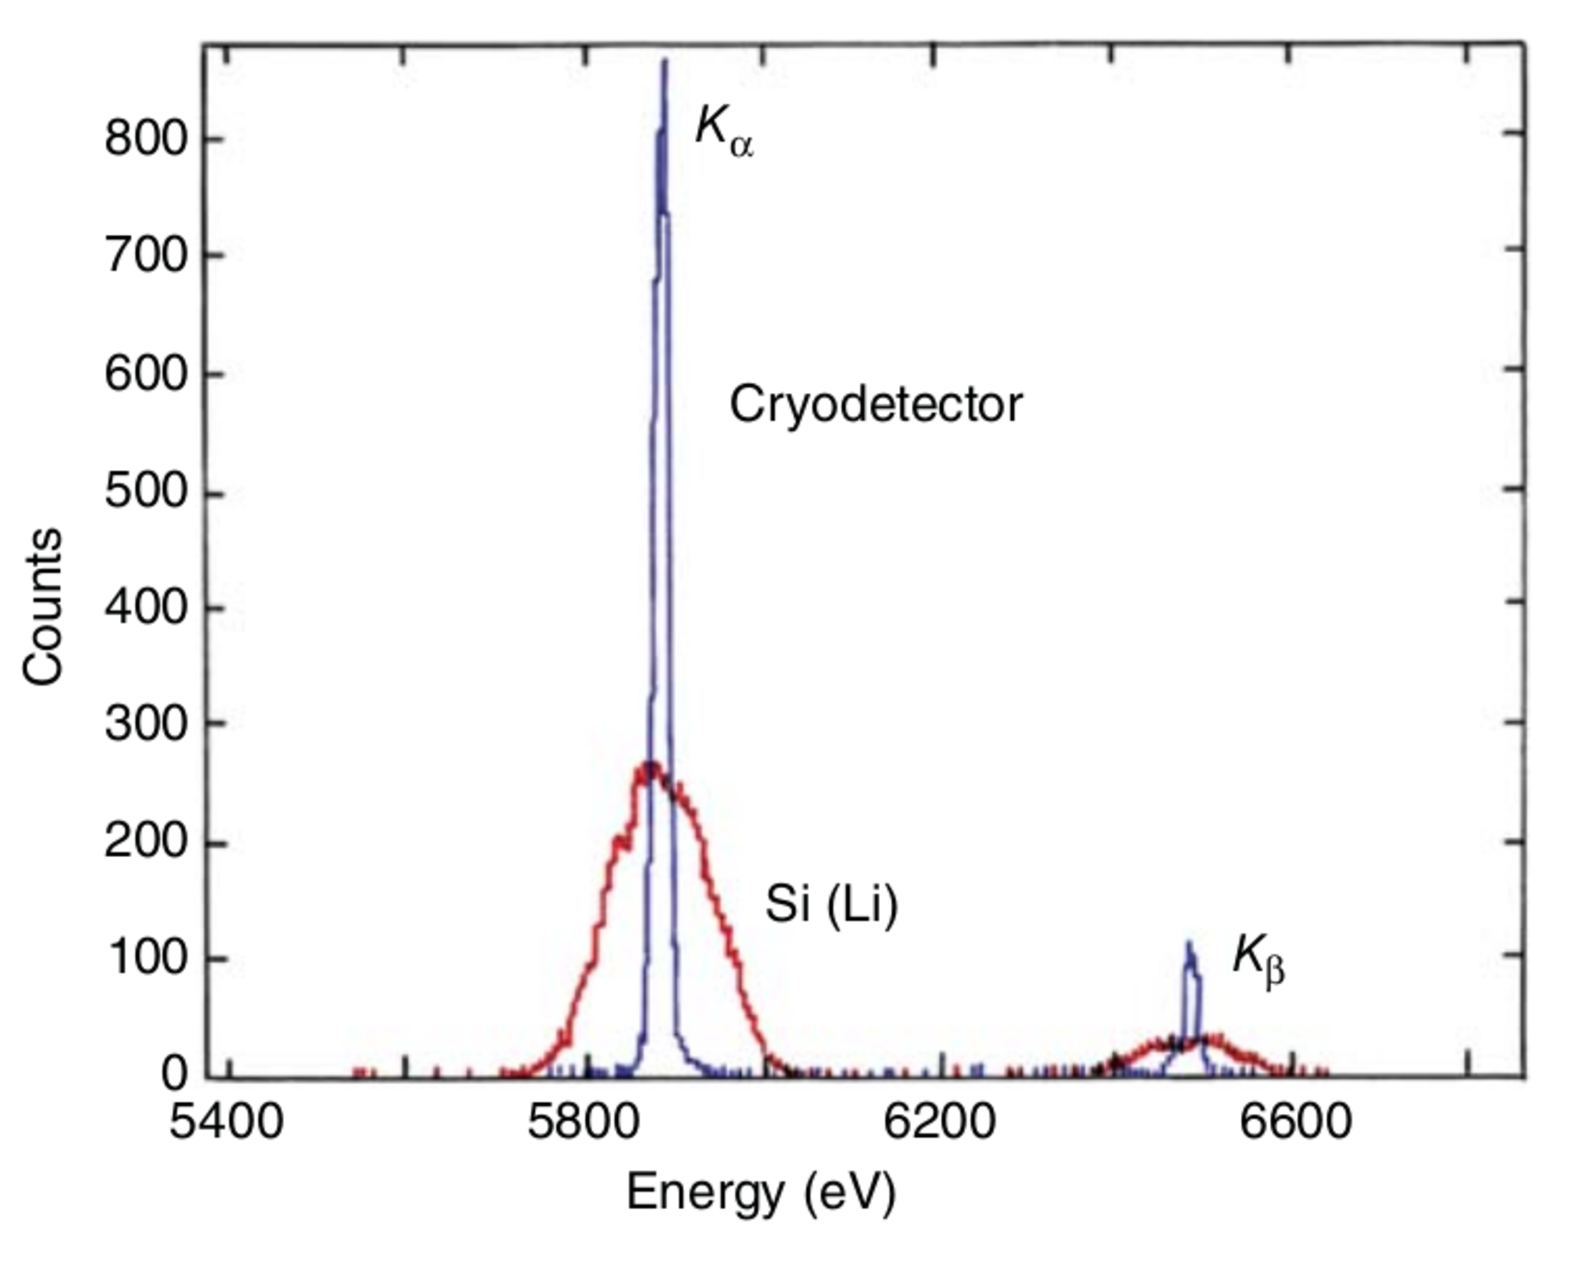
\includegraphics[height=0.48\textheight,width=0.48\textwidth]{criodet_vs_normal_det}}
																				\only<1>{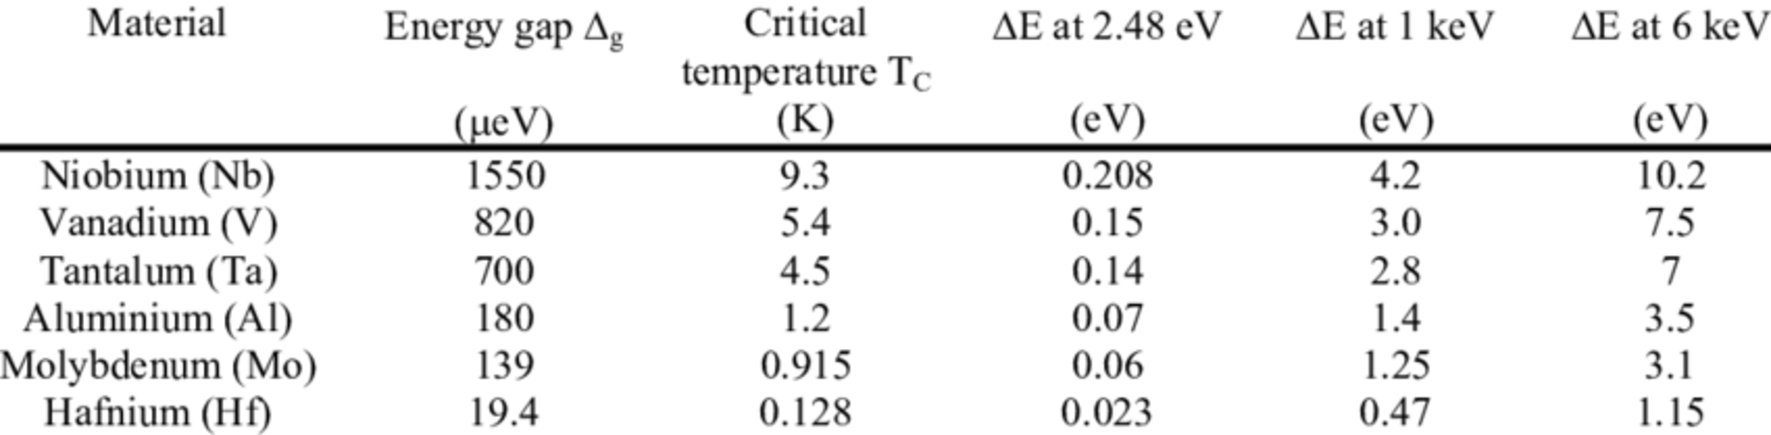
\includegraphics[height=0.22\textheight,width=0.50\textwidth]{energy_resolutions_sc}}
																\end{center}
																\pause
												\item[*] \alert{Sensibilidad energética:}
																Medida en que el detector es sensible a
																diferentes energías (longitudes de onda,
																frecuencia, ...)
																\begin{center}
																				\only<2>{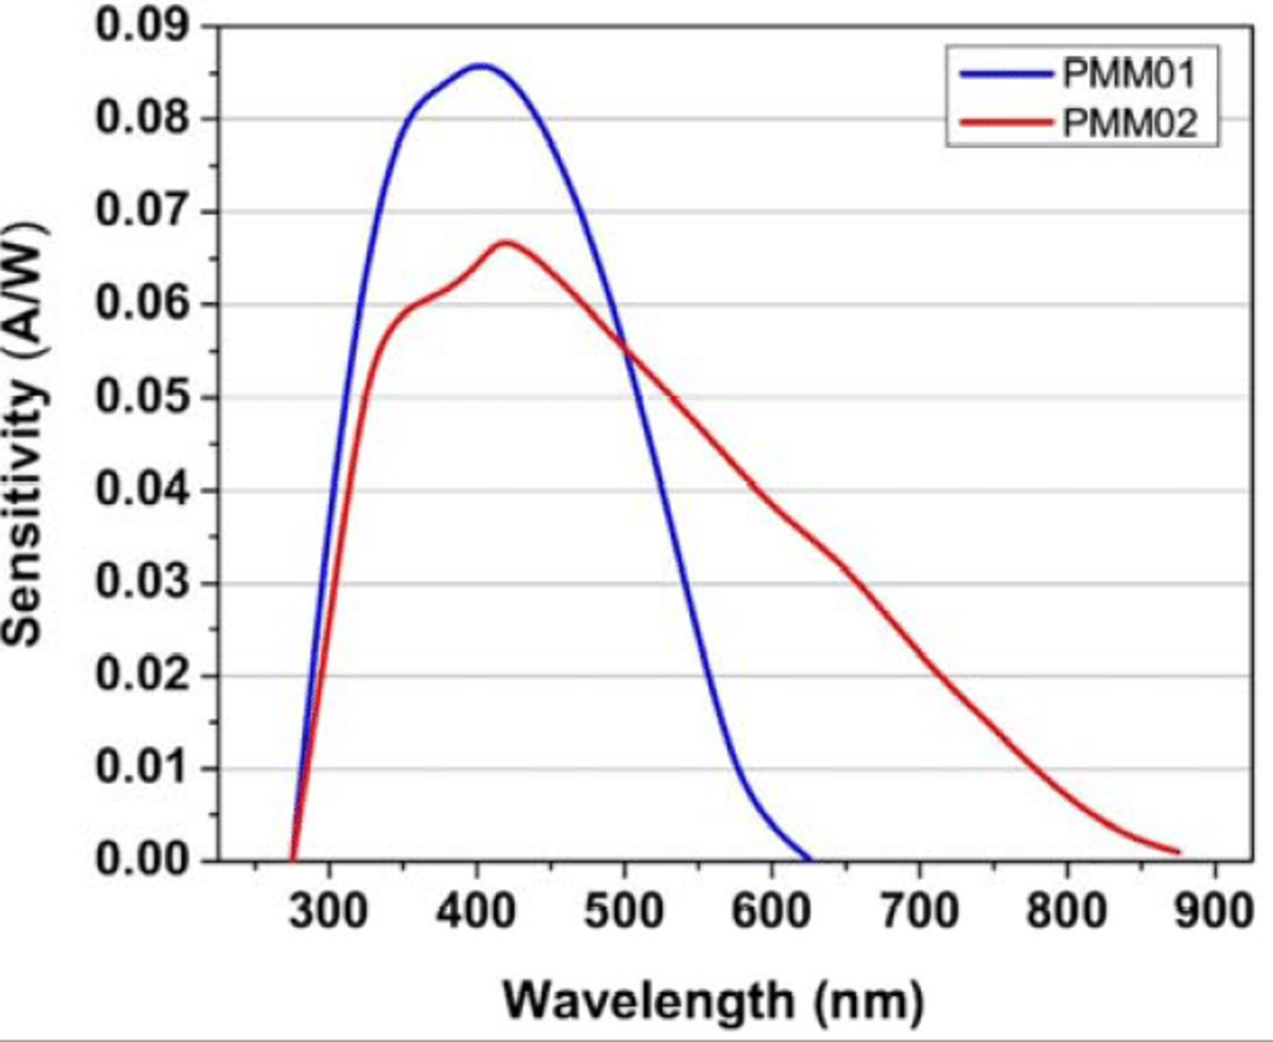
\includegraphics[height=0.48\textheight,width=0.48\textwidth]{spectral_response}}
																\end{center}
																\pause
												\item[*] \alert{Tiempo de respuesta:}
																\begin{itemize}
																				\item Resolución temporal:
																								Medida de la capacidad del
																								detector para distinguir dos
																								tiempos cercanos de arribo
																				\item Tasa de conteo: 
																								El detector es capaz de
																								registrar secuencias rápidas de
																								eventos
																\end{itemize}
												\item[*] \alert{Eficiencia de detección:}
																\begin{itemize}
																				\item Eficiencia de recolección:
																								Capacidad del detector de
																								capturar la radiación
																				\item Eficiencia cuántica: 
																								Medida en que el detector
																								convierte la energía entrante en
																								excitaciones finales
																\end{itemize}
																%									{\color[rgb]{0.00,0.21,0.47}RedPitaya}
								\end{itemize}
								%\end{exampleblock}
\end{frame}

%\begin{frame}
%				\frametitle{Comparación $\Delta E/E$}
%								\begin{center}
%												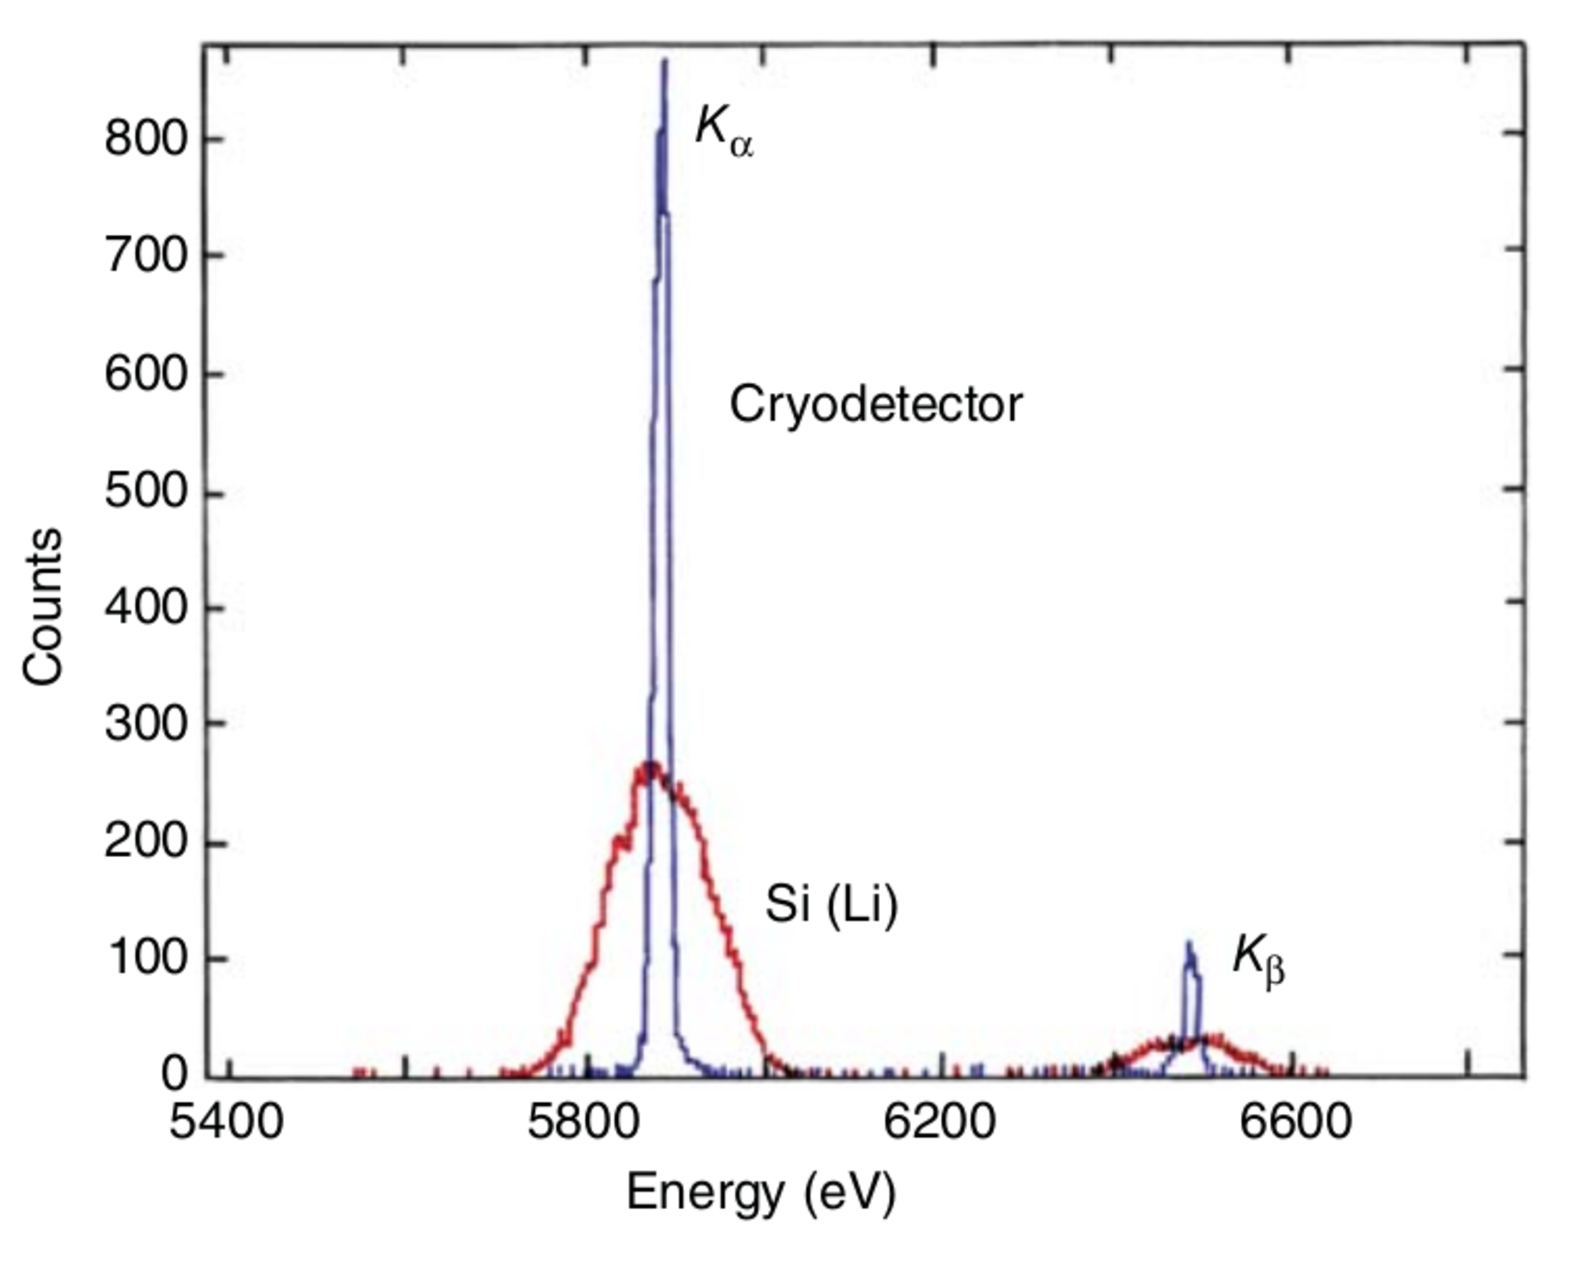
\includegraphics[height=0.48\textheight,width=0.50\textwidth]{criodet_vs_normal_det}
%												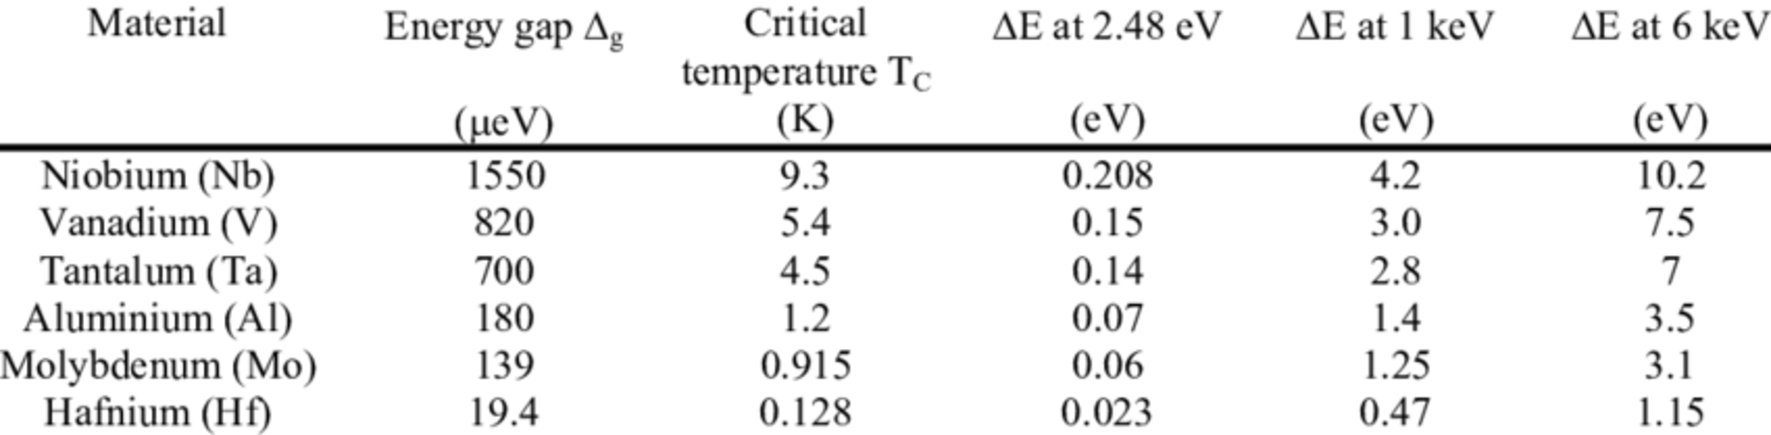
\includegraphics[height=0.24\textheight,width=0.50\textwidth]{energy_resolutions_sc}
%								\end{center}
%\end{frame} 

%------------------------------------------------------------------------------
\section{Superconductividad aplicada a detectores}
%------------------------------------------------------------------------------

\begin{frame}
				\frametitle{Superconductividad}
				\begin{alertblock}{Tres tipos de interacciones}
								\begin{itemize}
												\item Cuasipartículas
												\item Pares de Cooper
												\item Fonones
								\end{itemize}
				\end{alertblock}
				\begin{alertblock}{La superconductividad ofrece varios principios
								básicos para una detección efectiva de radiación:}
								\begin{itemize}
												\item creación de gran número de cuasipartículas por
																ruptura de {\color[rgb]{0.0,.5,.0}pares de Cooper}
												\item transición abrupta normal-superconductor 
												\item baja capacidad calorífica
												\item cambio de inductancia cinética
								\end{itemize}
				\end{alertblock}
\end{frame}

%\begin{frame}
%				\frametitle{Esquema de energía en cascada}
%				\begin{columns}
%								\begin{column}{0.9\textwidth}
%																\begin{itemize}
%																				\item 1er etapa: absorción de
%																								energía $\to$
%																								scattering electrón-electrón
%																								$\to$
%																								\alert{$10^{-15}$s}
%																				\item 2da etapa: conversión de
%																								energia $\to$ scattering
%																								electrón-electrón $\to$
%																								\alert{$10^{-12}$s}
%																				\item 3ra etapa: evolución de la
%																								distribución mixta de pares
%																								qp-ph $\to$
%																								\alert{$10^{-9} - 10^{-6}$s} 
%																				\item 4ta etapa: termalización $\to$
%																								fonones térmicos $\to$
%																								\alert{$10^{-3}$s} 
%																\end{itemize}
%								\end{column} \ \
%							%	\begin{column}{0.3\textwidth}
%							%									\begin{itemize}
%							%													\item 			\\
%							%													\item 			scattering electrón-fonón\\
%							%													\item 
%							%													\item  fonones térmicos
%							%									\end{itemize}
%							%	\end{column}
%				\end{columns}
%				CClasificación de detectores superconductores\\
%				Bolometros o detectores térmicos \hspace{2cm} Detectores de
%				no-equilibrio\\
%				4ta etapa \hspace{3cm} 2da-3ra etapas
%\end{frame}

\begin{frame}
				\frametitle{Tipos de detectores superconductores}
\begin{itemize}
				\item \alert{T}ransition \alert{E}dge
								\alert{S}ensor (TES)
				\item Transiciones
								superconductor-aislante-superconductor
								(SIS) $\to$ \alert{S}uperconducting
								\alert{T}unnel \alert{J}unction
								(STJ)
				\item \alert{H}ot
								\alert{E}lectron
								\alert{S}uperconducting
								\alert{P}hotodetector (HESP)
				\item \alert{S}uperconducting
								\alert{H}ot
								\alert{E}lectron
								\alert{B}olometers (HEB)
				\item Calorímetros
								criogénicos
%				\item Transiciones
%								superconductor-aislante-superconductor
%								(SIS)
				\item \alert{M}icrowave \alert{K}inetic \alert{I}nductance \alert{D}etector (MKID)

\end{itemize}
				\begin{block}{}
								\alert{Los principales parámetros físicos que caracterizan a los HEB, los 
								bolómetros TES y a los microcalorímetros son la capacidad de
								respuesta y el ruido}
				\end{block}
\end{frame}

\begin{frame}
				\frametitle{Tipos de detectores superconductores}
				\begin{columns}
								\begin{column}{0.67\textwidth}
												\begin{block}{}
																\begin{itemize}
																				\item \underline{\alert{T}ransition \alert{E}dge
																								\alert{S}ensor}:\\
																								{\color[rgb]{0,0.5,0}Transición aguda
																								normal-superconductor $\to$
																								cambio de resistencia}
																				\item \underline{\alert{S}uperconducting
																								\alert{T}unnel \alert{J}unction}: \\
																								{\color[rgb]{0,0.5,0}Ruptura de pares de Cooper $\to$
																								creación de quasipartículas en
																								exceso $N \sim \Delta E/E$}
																				\item \underline{\alert{H}ot
																								\alert{E}lectron
																								\alert{S}uperconducting
																								\alert{P}hotodetector}:\\
																								{\color[rgb]{0,0.5,0}Creación de puntos calientes
																								$\to$	transición inducida por
																								corriente o cambio de
																								inductancia cinética}
																				\item \underline{\alert{S}uperconducting
																								\alert{H}ot
																								\alert{E}lectron
																								\alert{B}olometers}
																\end{itemize}
												\end{block}
								\end{column} \ \
								\begin{column}{0.33\textwidth}
												\begin{center}
																\only<1>{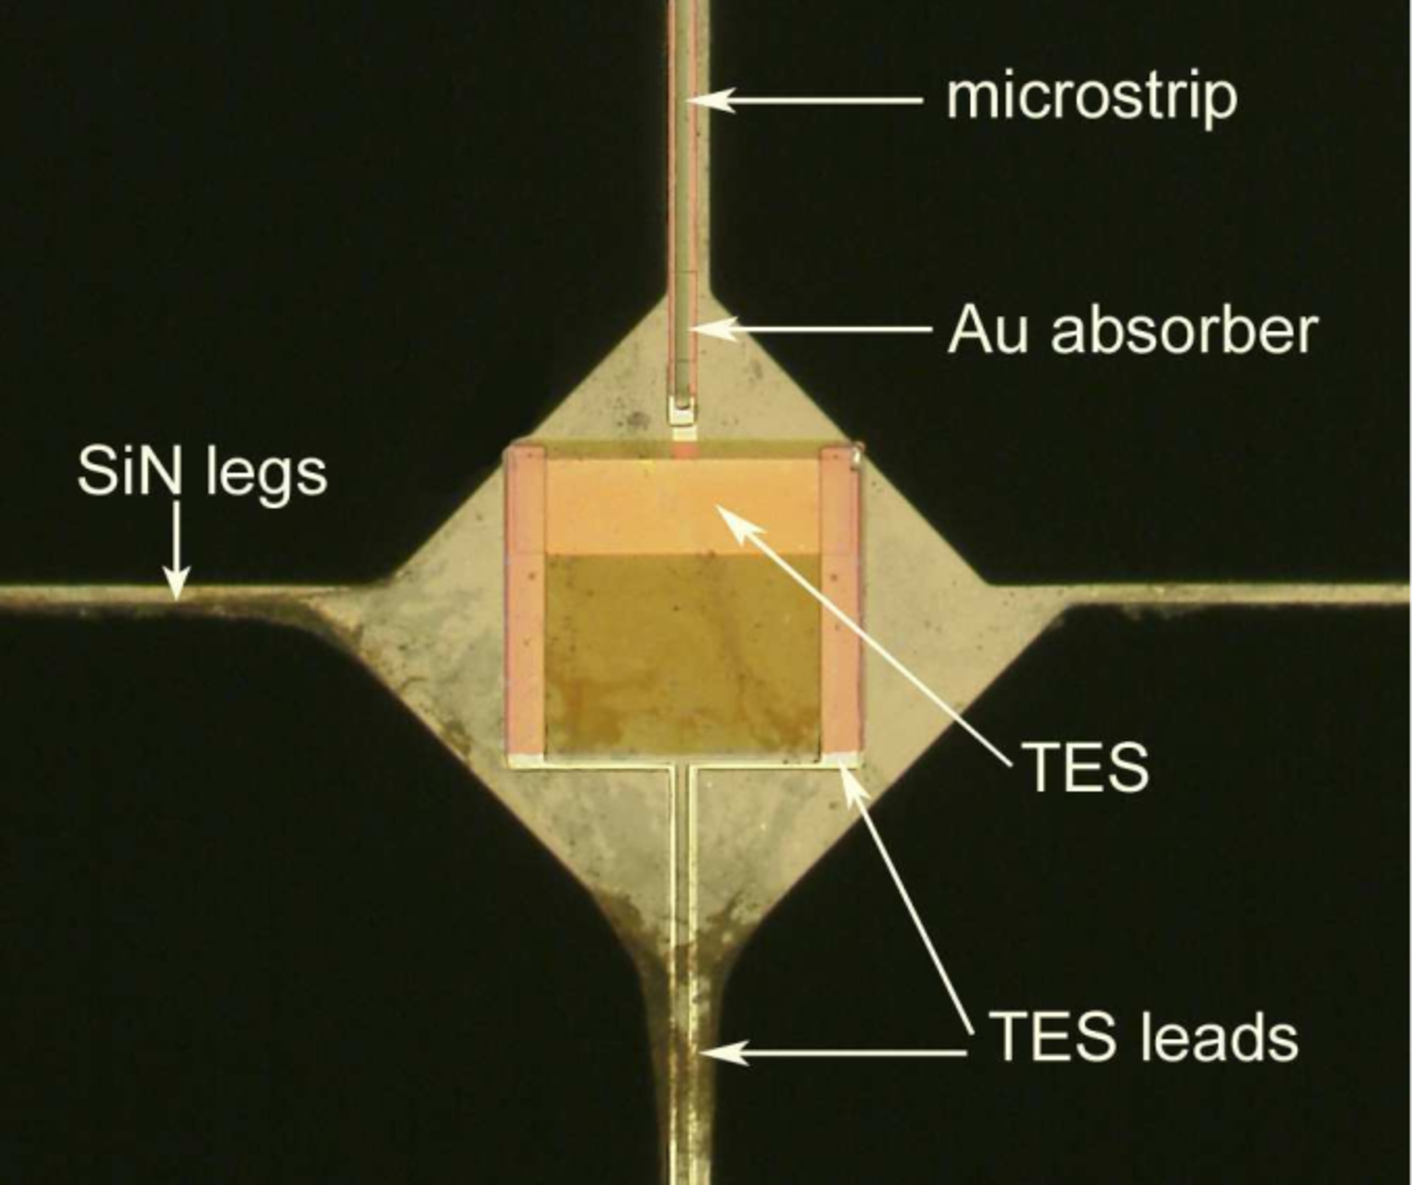
\includegraphics[height=0.43\textheight,width=0.9\textwidth]{sensor_TES}}
																\only<2>{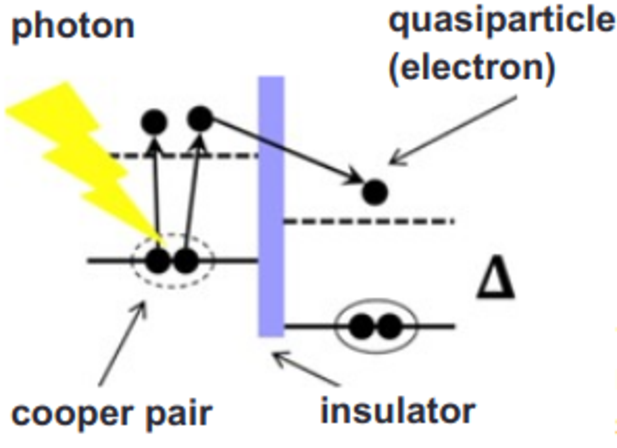
\includegraphics[height=0.28\textheight,width=0.8\textwidth]{stj_2}}
																\only<2>{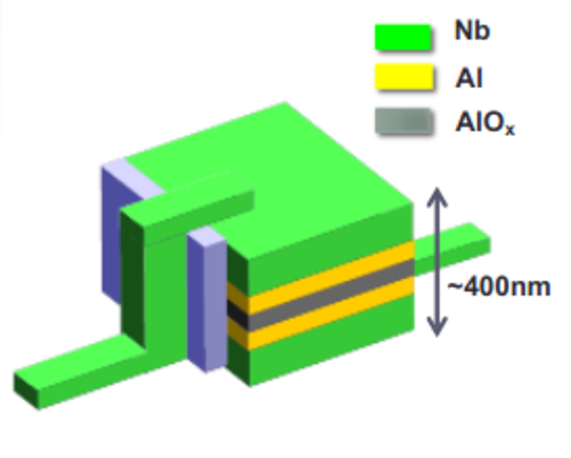
\includegraphics[height=0.28\textheight,width=0.8\textwidth]{stj_1}}
												\end{center}
								\end{column}
				\end{columns}
\end{frame}

%Esto es sacado del libro de seidel
\begin{frame}
				\frametitle{Calorímetro criogénico}
				Componentes básicos $\to$ absorbente, termómetro y un enlace térmico al
				baño de calor\\
				Por ej: $\text{TeO}_2$ como cristal absorbente (a 15 mK) para detectar
				partículas $\alpha$ y $\gamma$
				\begin{columns}
								\begin{column}{0.35\textwidth}
												Si $\Delta E$ es la energía absorbida, resulta en un
												cambio de temperatura\\ \vspace{0.5cm} \alert{$\Delta T = \frac{\Delta
												E}{m\cdot c}$}\\\vspace{.5cm}
												c $\to$ capacidad calorífica específica\\
												m $\to$ masa del calorímetro
								\end{column}
								\begin{column}{0.65\textwidth}
								\begin{center}
												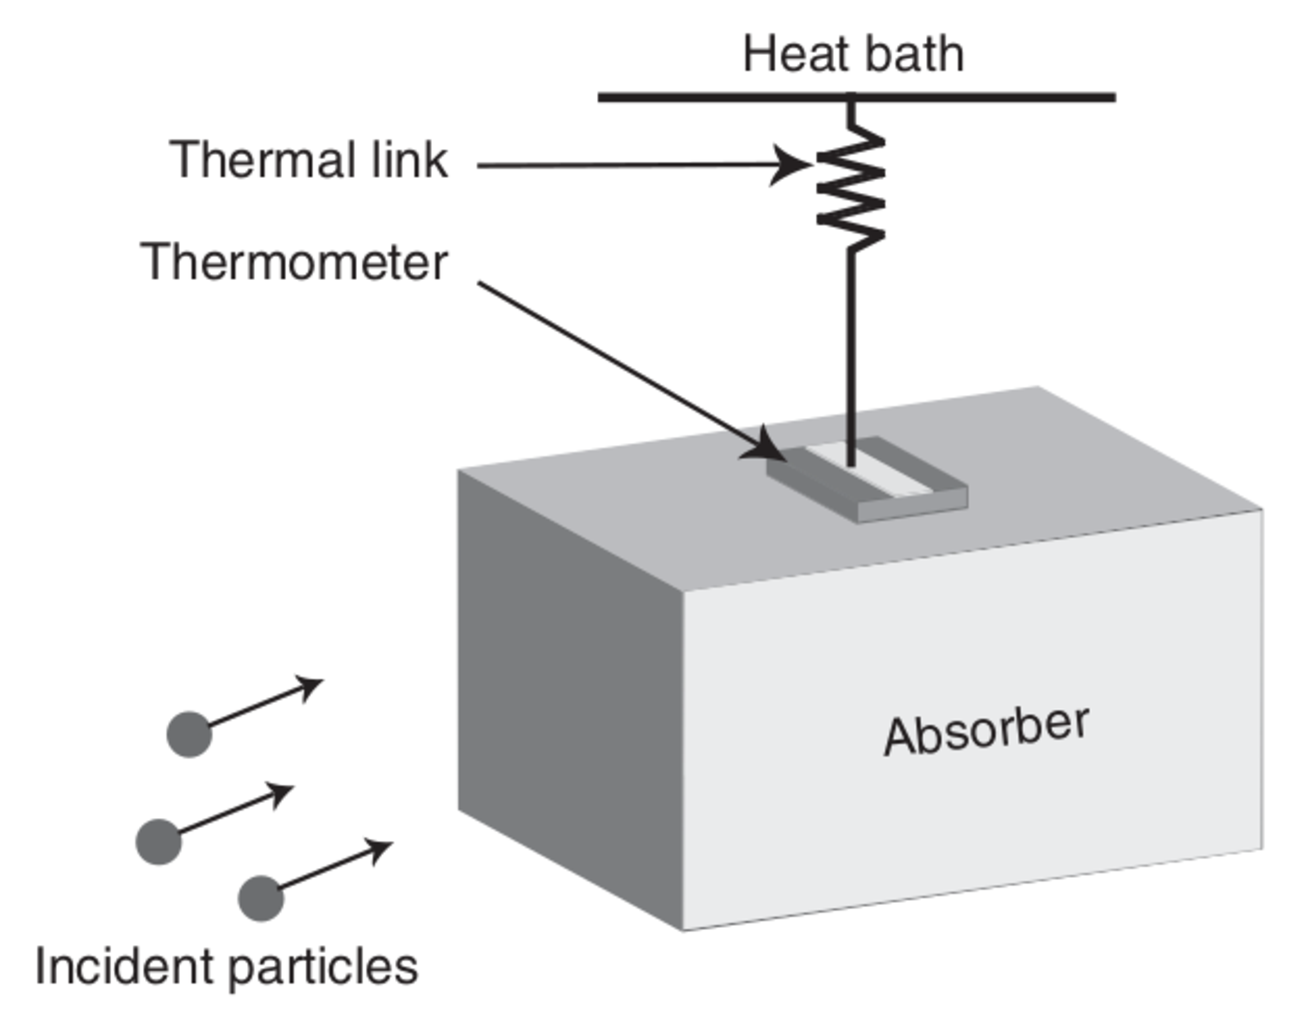
\includegraphics[height=0.58\textheight,width=0.7\textwidth]{microcalorimetro}
								\end{center}
								\end{column}
				\end{columns}
\end{frame} 

\begin{frame}
				\frametitle{TES}
				Detecta la radiación por medio de un absorbente con capacidad calorífica
				C, que convierte la potencia de radiación P en calor.\\
				Aumento de temperatura \alert{$\to \Delta T = \frac{P}{G}$}\\

				G $\to$ conductancia térmica del disipador

        La señal eléctrica se obtiene de un termistor acoplado al absorbedor 
				%acoplado al absorbedor. Los TES suelen ser detectores directos (es
				%decir, incoherentes), mientras que los HEB superconductores se usan más
				%a menudo como detectores indirectos (es decir, coherentes o
				%mezcladores), aunque la detección directa también es posible con los HEB
				%superconductores.
								\begin{center}
												\only<1>{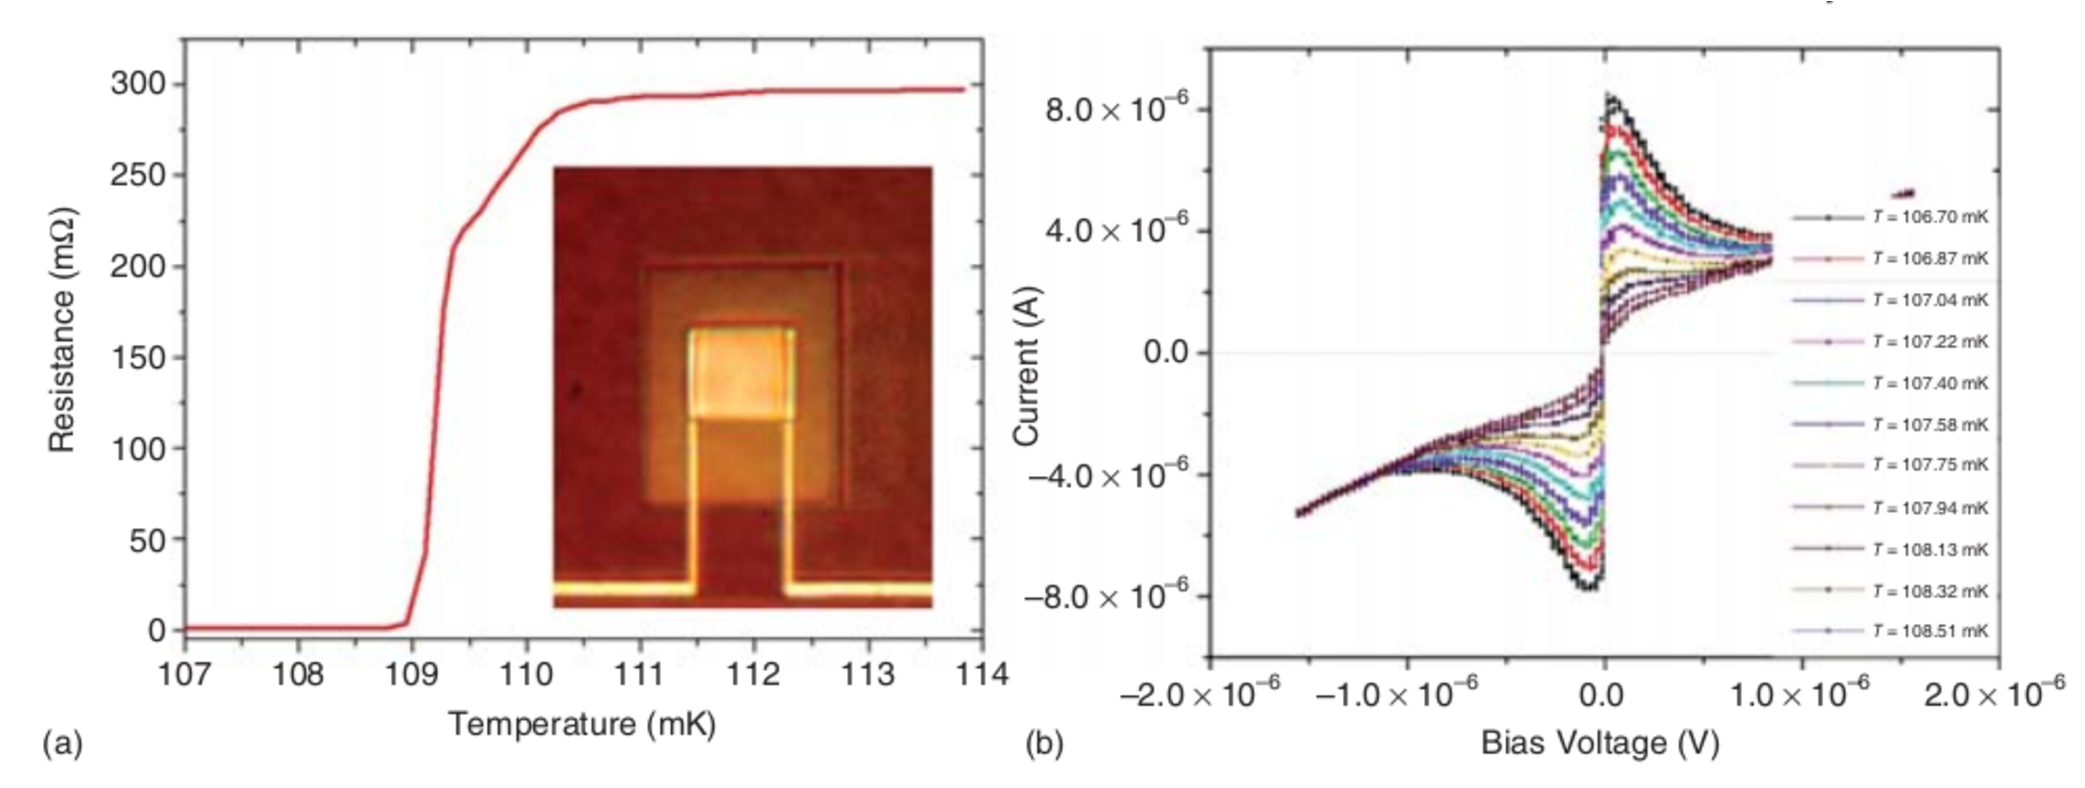
\includegraphics[height=0.48\textheight,width=0.9\textwidth]{TES_libro}}
												\only<2>{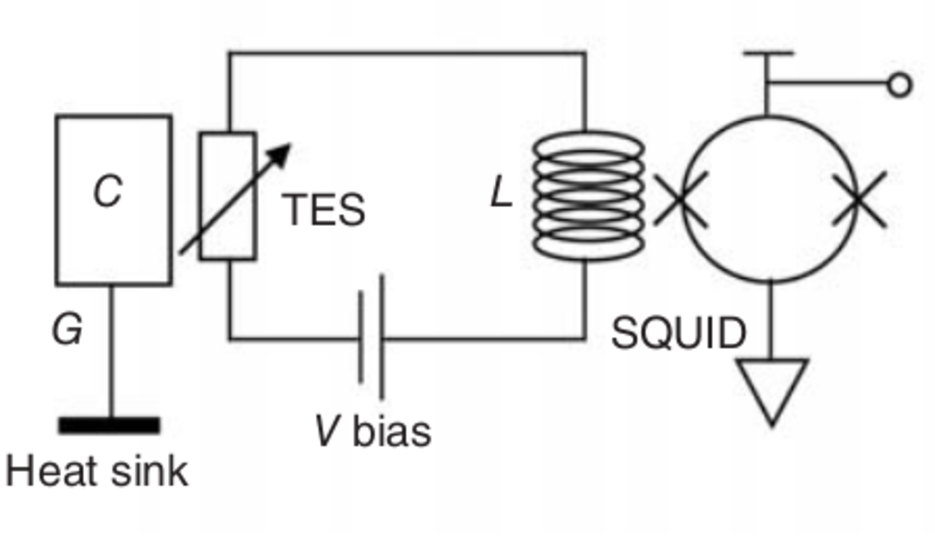
\includegraphics[width=0.4\textwidth]{TES_readout}}
												\only<2>{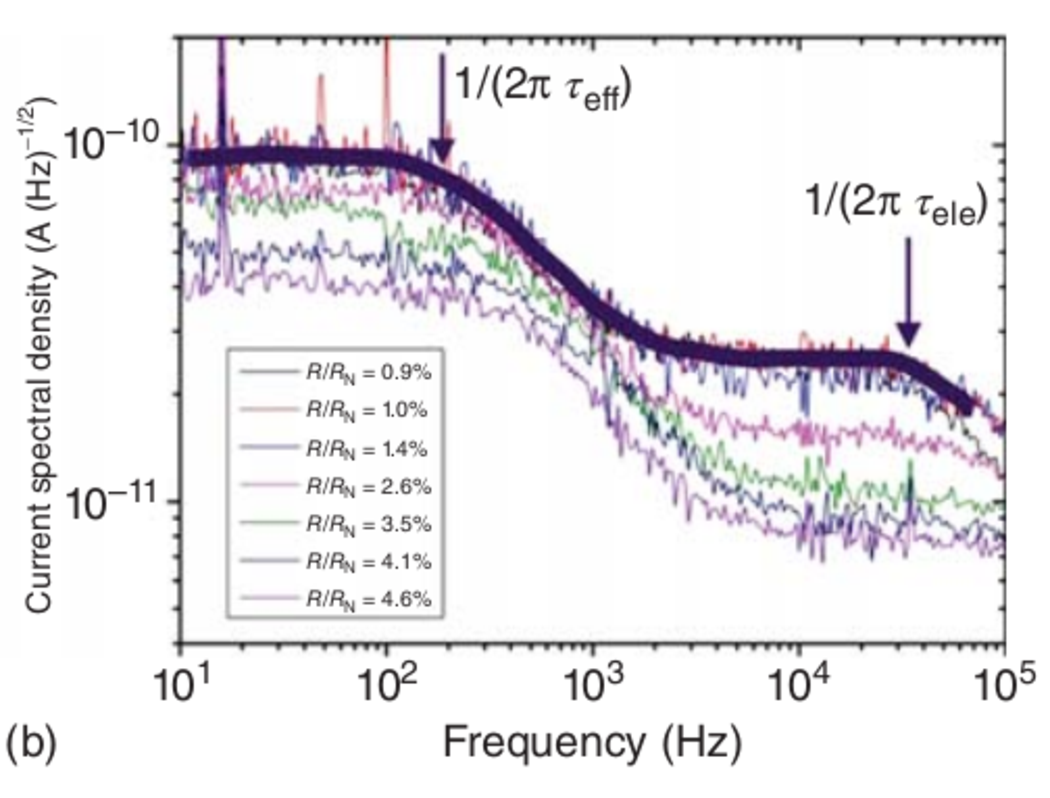
\includegraphics[width=0.4\textwidth]{TES_NEP}}
								\end{center}
\end{frame} 

%\begin{frame}
%				\frametitle{TES}
%				\begin{columns}
%								\begin{column}{0.75\textwidth}
%												\begin{block}{}
%																\begin{itemize}
%																				\item Matriz de micro-resonadores pixelado
%																				\item Detectores superconductores: operados a $<
%																								300\,\text{mK}$
%																				\item Sensible a fotones y fonones
%																				\item Al acoplar la inductancia cinética a un
%																\end{itemize}
%												\end{block}
%								\end{column} \ \
%								\begin{column}{0.25\textwidth}
%												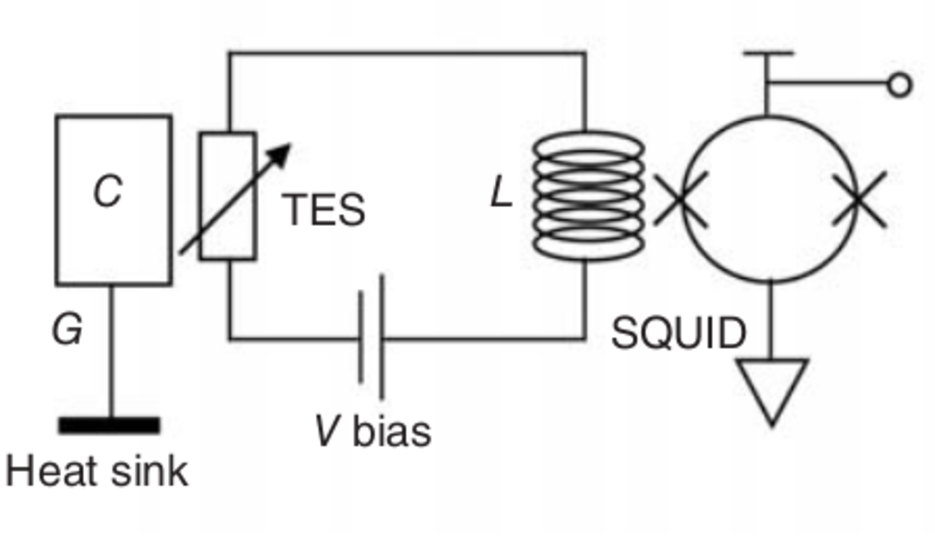
\includegraphics[width=0.8\textwidth]{TES_readout}
%												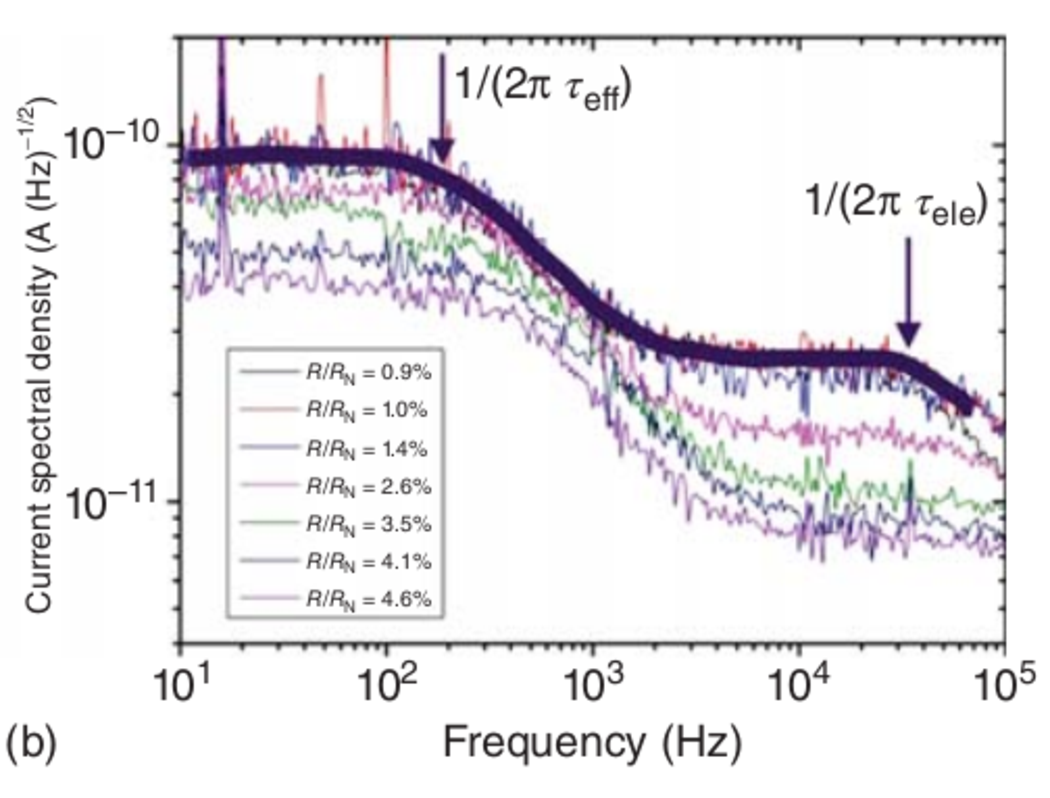
\includegraphics[width=0.8\textwidth]{TES_NEP}
%								\end{column}
%				\end{columns}
%\end{frame}

\begin{frame}
				\frametitle{Mezclador Hot Electron Bolometer (HEB)}
				\begin{block}{Principio de operación}
				\begin{itemize}
								\item La radiación calienta los electrones
								\item Enfriamiento ya sea por fonones o por difusión
								\item Detección directa o heterodina
				\end{itemize}
				\end{block}
								\begin{center}
												\only<1>{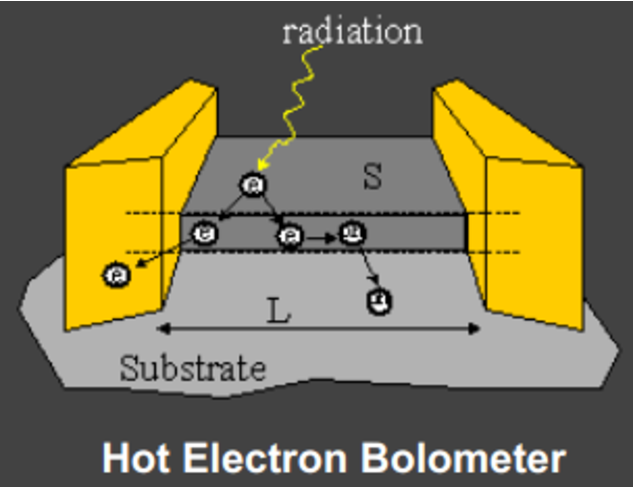
\includegraphics[height=0.4\textheight,width=0.4\textwidth]{heb_bolometer}}
												\only<2>{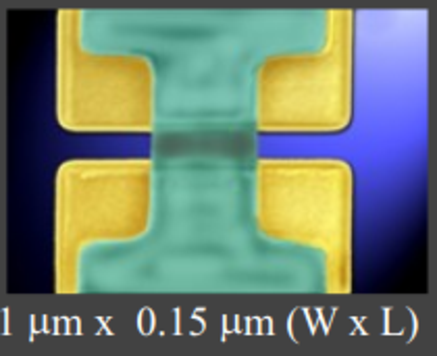
\includegraphics[height=0.3\textheight,width=0.3\textwidth]{heb_bolometer2}}
												\only<2>{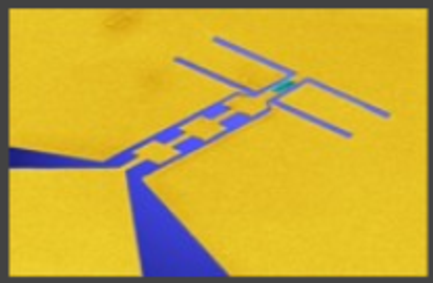
\includegraphics[height=0.3\textheight,width=0.3\textwidth]{heb_bolometer3}}
								\end{center}
\end{frame} 

\begin{frame}
				\frametitle{Mezclador Hot Electron Bolometer (HEB)}
				\begin{itemize}
								\item Puente superconductor (\alert{Nb, NbN,
												NbTiN, Al, YBCO}) con dimensiones nm o sub-$\mu$m,
												puesto en contacto con gruesas almohadillas de oro.
				\end{itemize}
								\begin{center}
												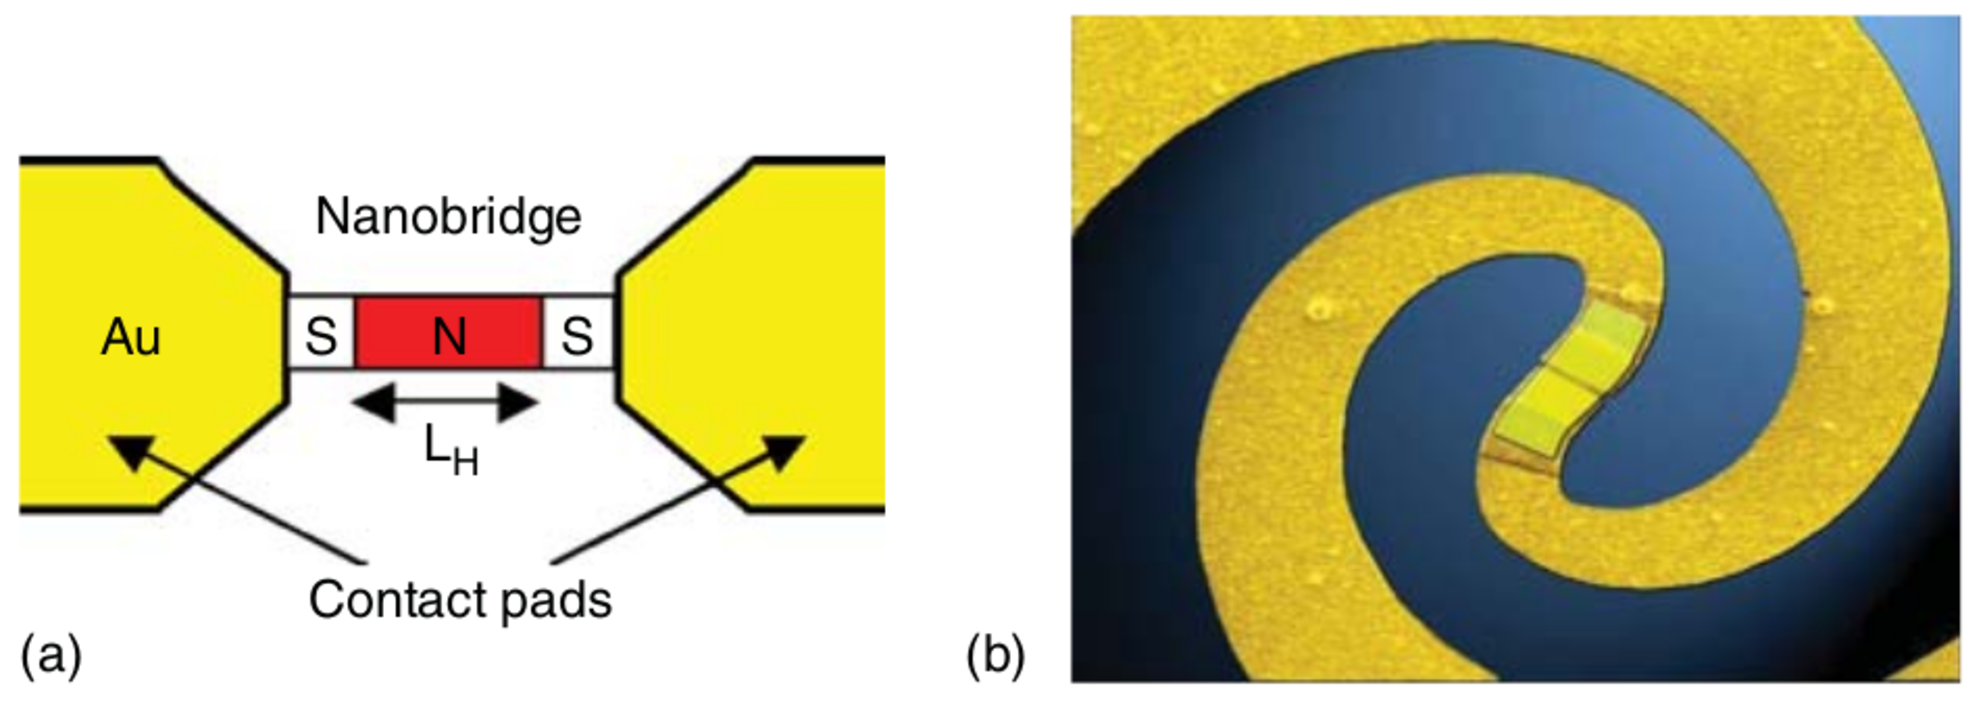
\includegraphics[height=0.48\textheight,width=0.9\textwidth]{heb_mixer}
								\end{center}
\end{frame} 

\begin{frame}
				\frametitle{Mezclador Hot Electron Bolometer (HEB)}
				\begin{itemize}
								\item Usado por encima de $\sim$ 1200 GHz en el régimen THz
								\item Mejor performance que los SIS por encima de 1200 GHz
								\item Teoría aún no bien entendida
								\item Investigación activa en este campo
				\end{itemize}
								\begin{center}
												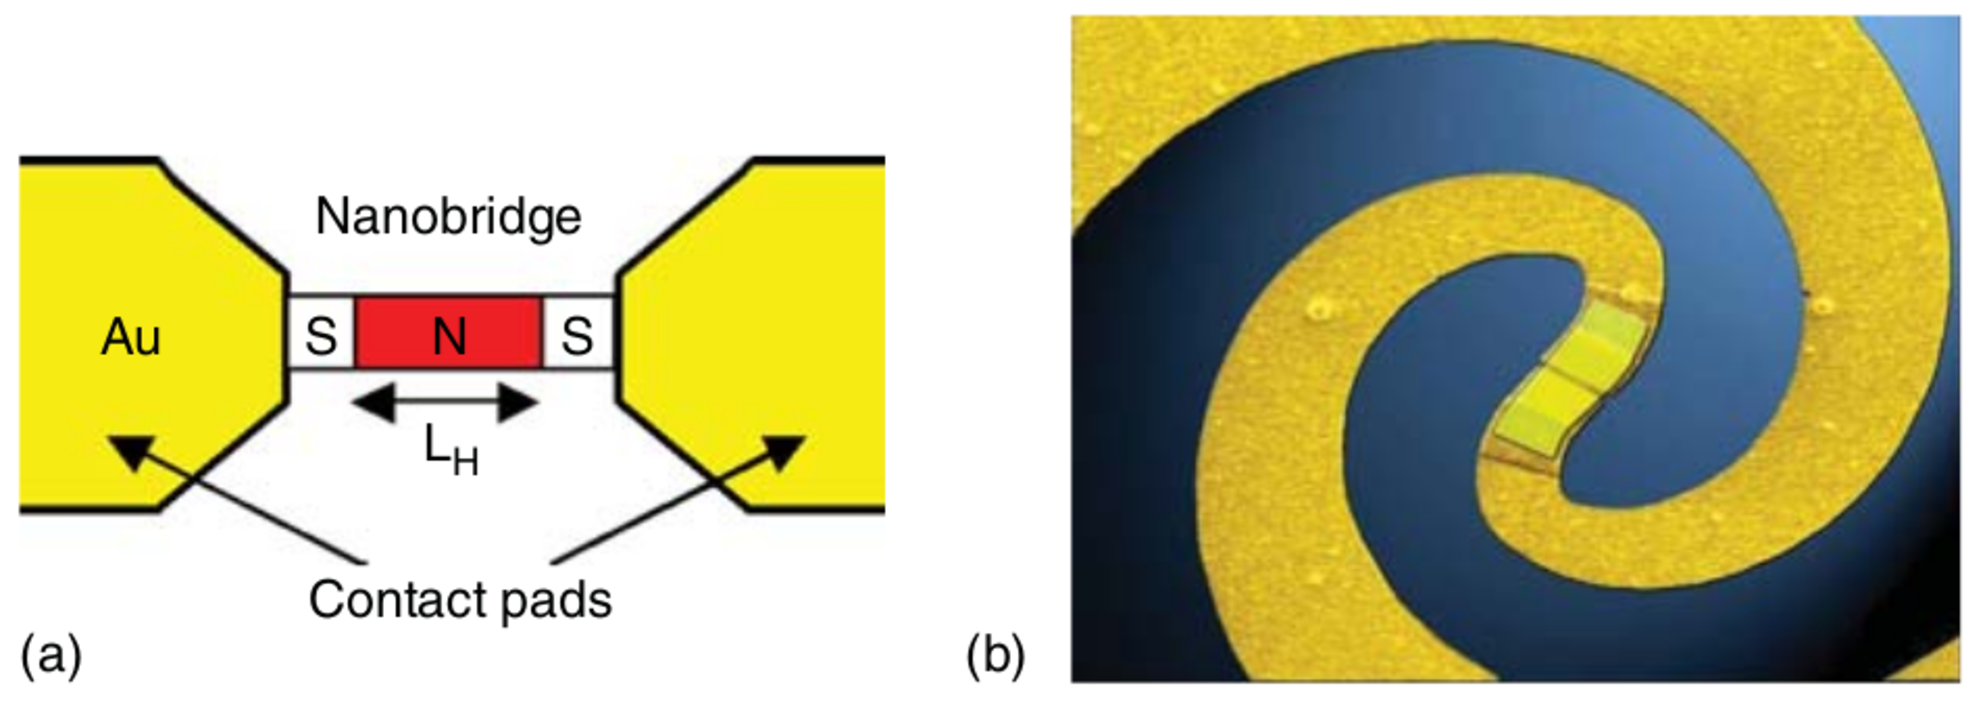
\includegraphics[height=0.48\textheight,width=0.9\textwidth]{heb_mixer}
								\end{center}
\end{frame} 

\begin{frame}
				\frametitle{Bolómetros (de inductancia cinética)}
								\begin{center}
												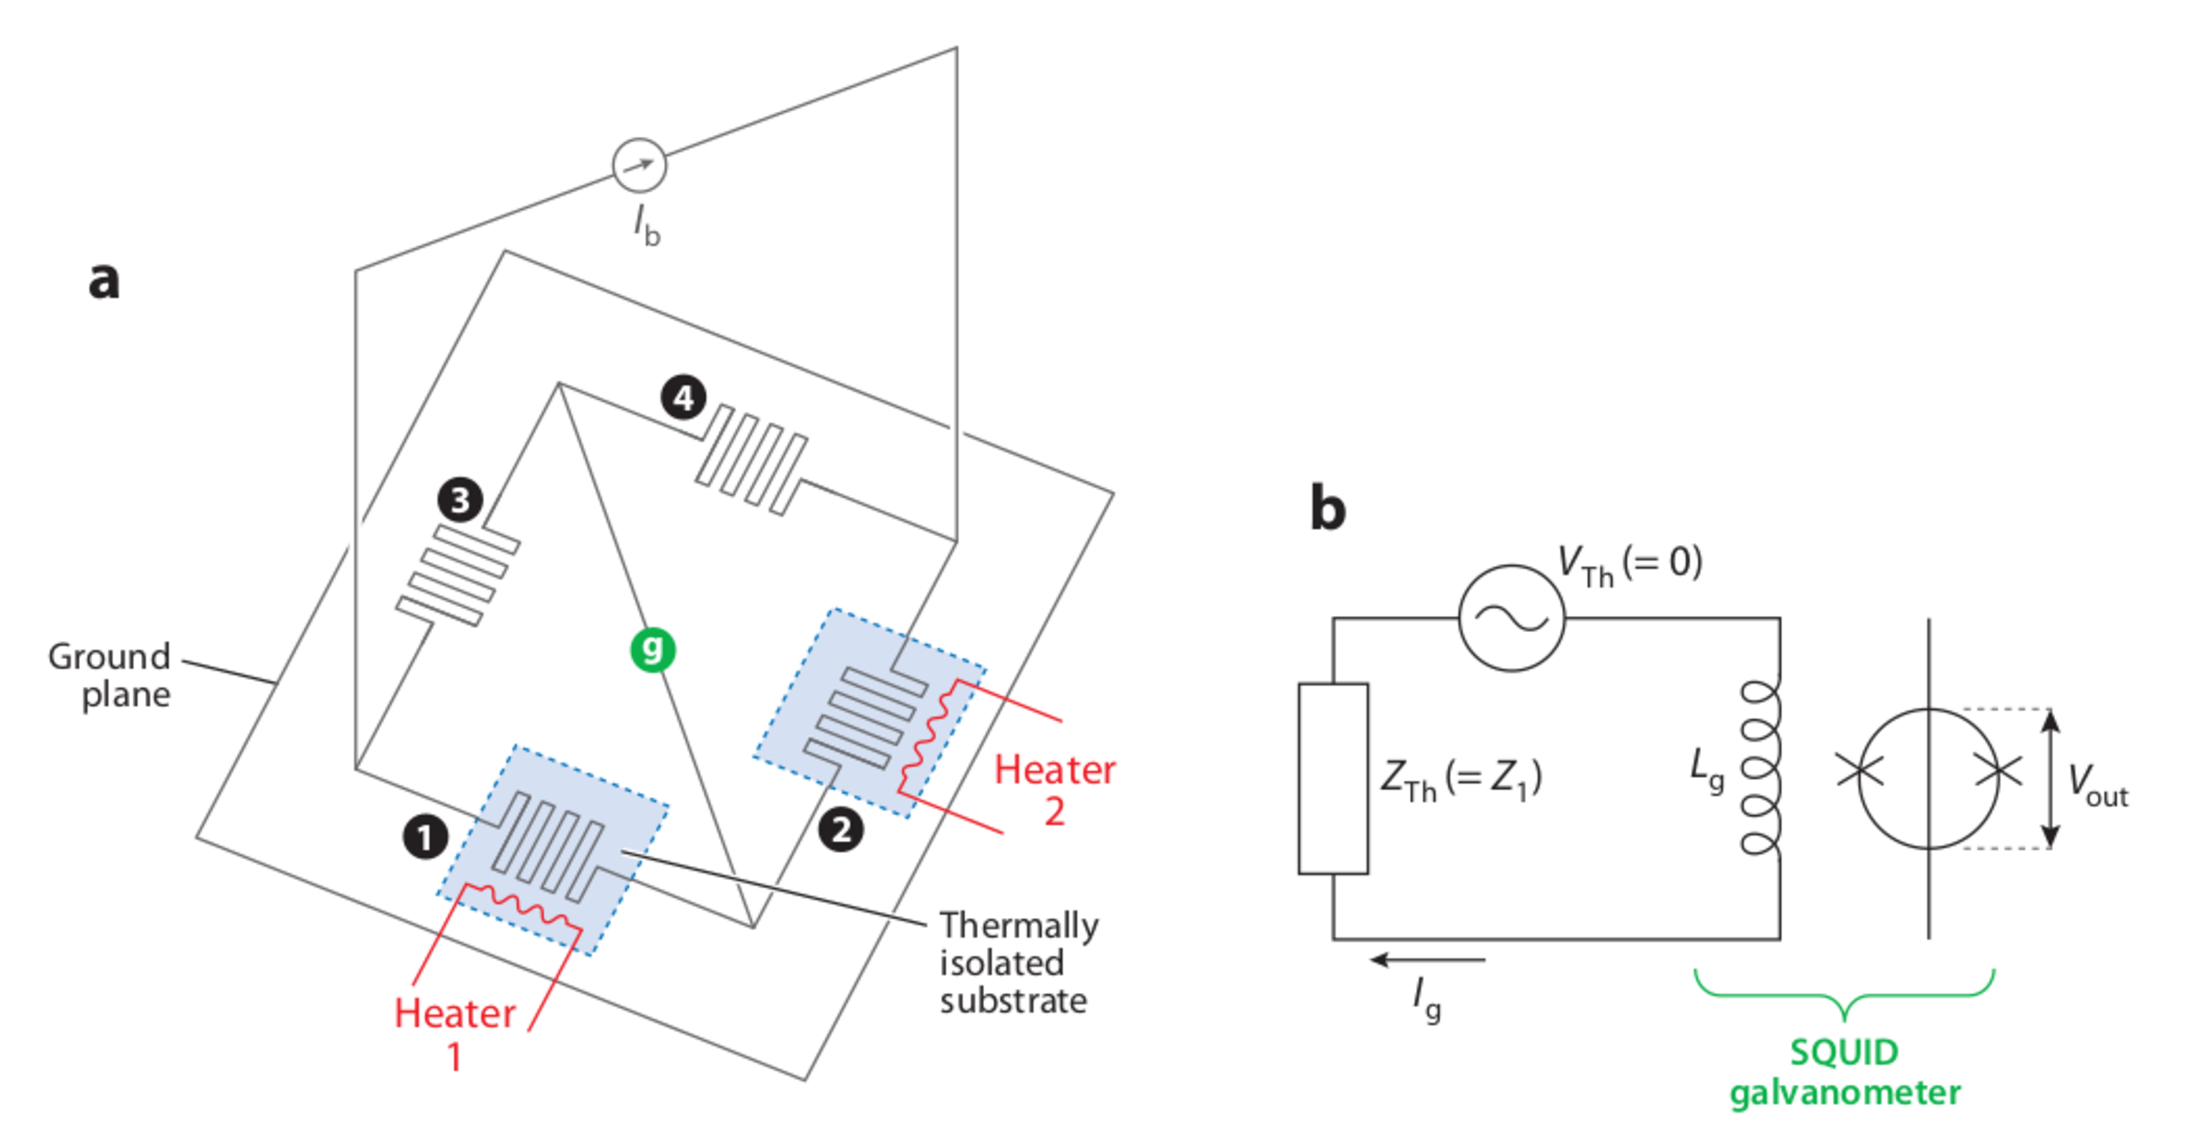
\includegraphics[height=0.48\textheight,width=0.9\textwidth]{detector_bolometro_kid}
								\end{center}
								Los inductores superconductores 1, 2, 3 y 4 están
								dispuestos en una configuración de \alert{puente de Wheatstone}. 
								El puente se excita con un generador de CA $I_b$ y se lee con el
								galvanómetro \alert{SQUID}
\end{frame} 

\begin{frame}
				\frametitle{Mezcladores SIS}
				Han reemplazado a los mezcladores de diodos Schottky en la mayoría de
				los radio-observatorios\\
				Algunos materiales $\to$ $Al-Al_2 O_3-Pb$
								\begin{center}
												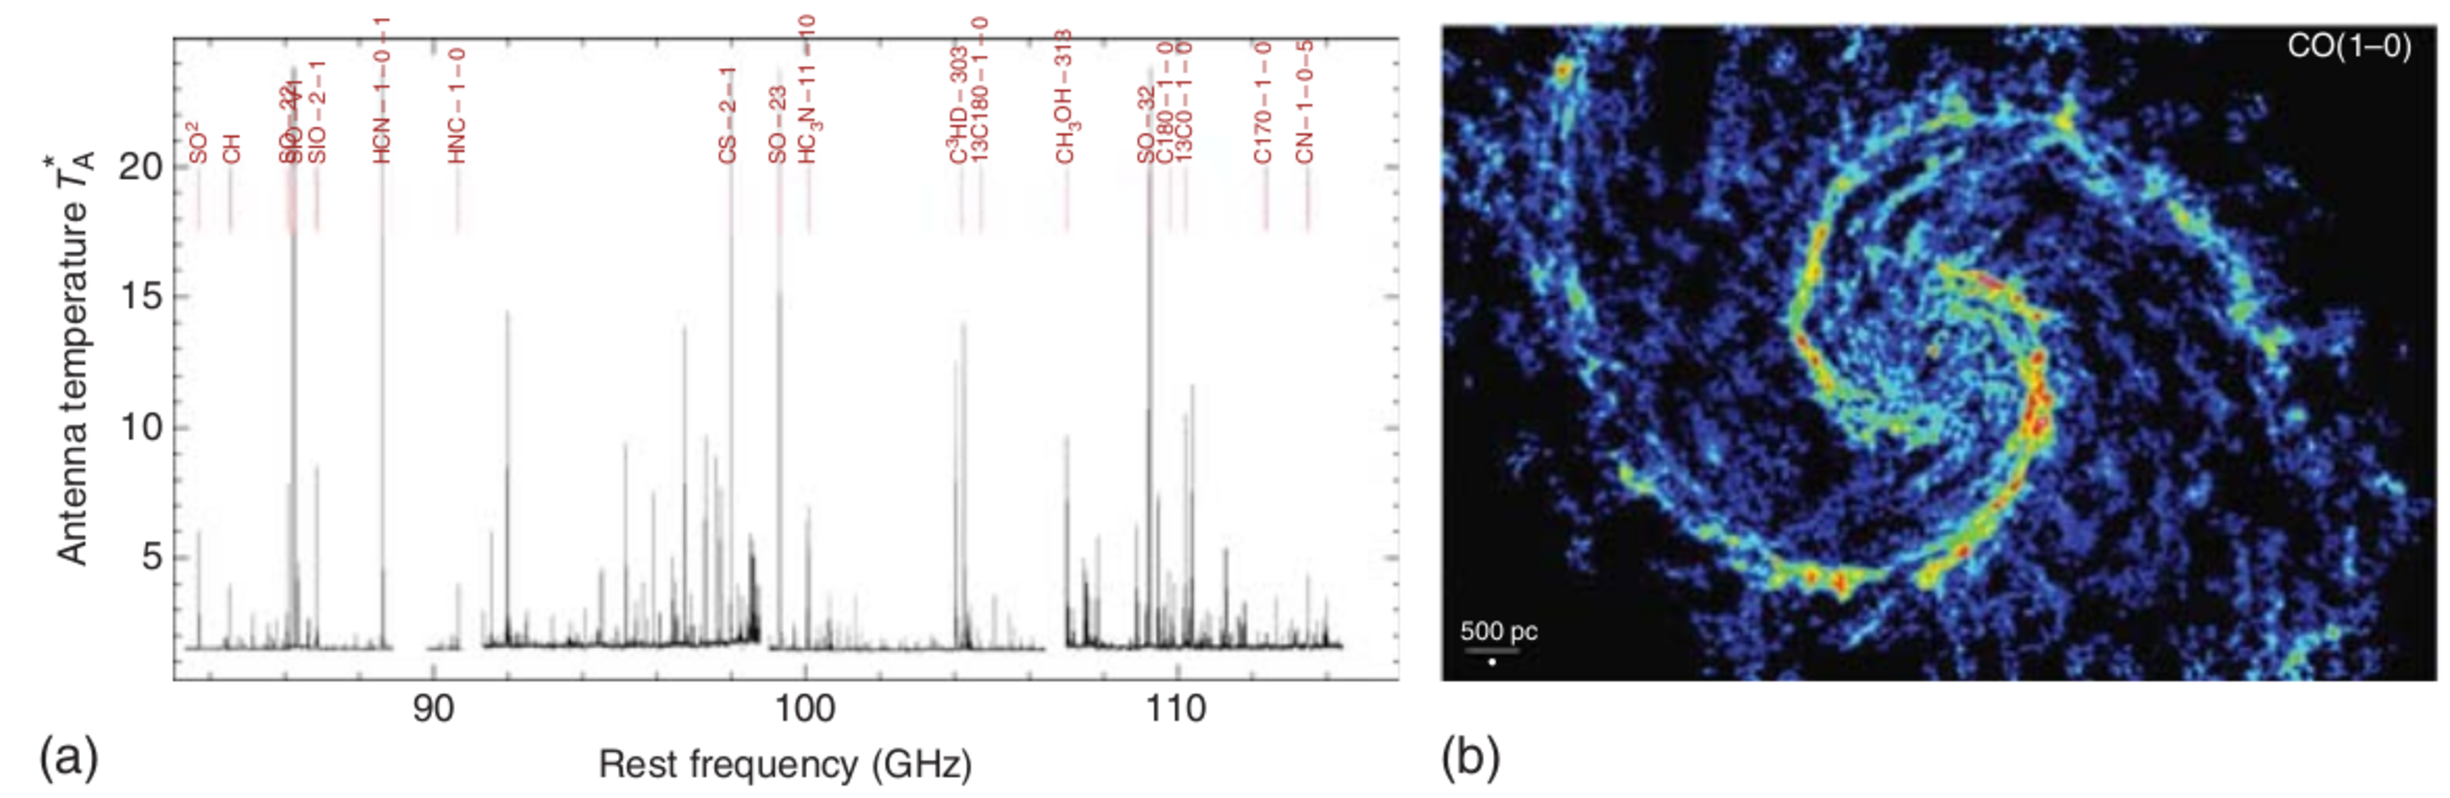
\includegraphics[height=0.38\textheight,width=0.9\textwidth]{sis_mixers}
								\end{center}
								Ejemplo de observaciones astronómicas hechas con mezcladores
								SIS.
\end{frame} 

\begin{frame}
				\frametitle{Mezcladores SIS}
				\begin{itemize}
								\item Usados en mm y sub-mm, desde $\sim$ 70 GHz a $\sim$ 1200
												GHz
								\item Muy buena performance
								\item Teoría bien entendida
								\item Tecnología sub-mm elegida para telescopios espaciales y
												terrestres
								\item \alert{Principio: tunneling asistido por fotones}
				\end{itemize}
								\begin{center}
												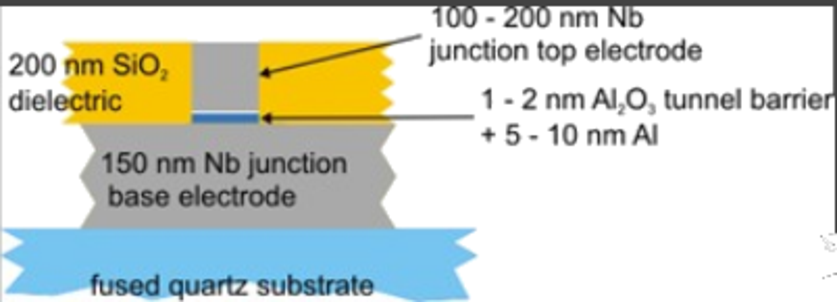
\includegraphics[height=0.3\textheight,width=0.4\textwidth]{sis_mixer}
								\end{center}
								El SIS es una estructura tipo sandwich con un aislante muy
								fino\\
								\alert{Espesor del aislante $\leq$ 1 mm : tunneling}
\end{frame} 
%------------------------------------------------------------------------------
%\section{Amplificador lock-in}
%------------------------------------------------------------------------------

\begin{frame}
				\frametitle{Micro-resonadores superconductores}
				\begin{itemize}
								\item $Q_s \to$ factor de calidad superficial\\
								\item Lograr altos Q requiere minimizar las fuentes disipación,
												incluida la pérdida debida a la radiación en el espacio
												libre
				\end{itemize}
								\begin{center}
												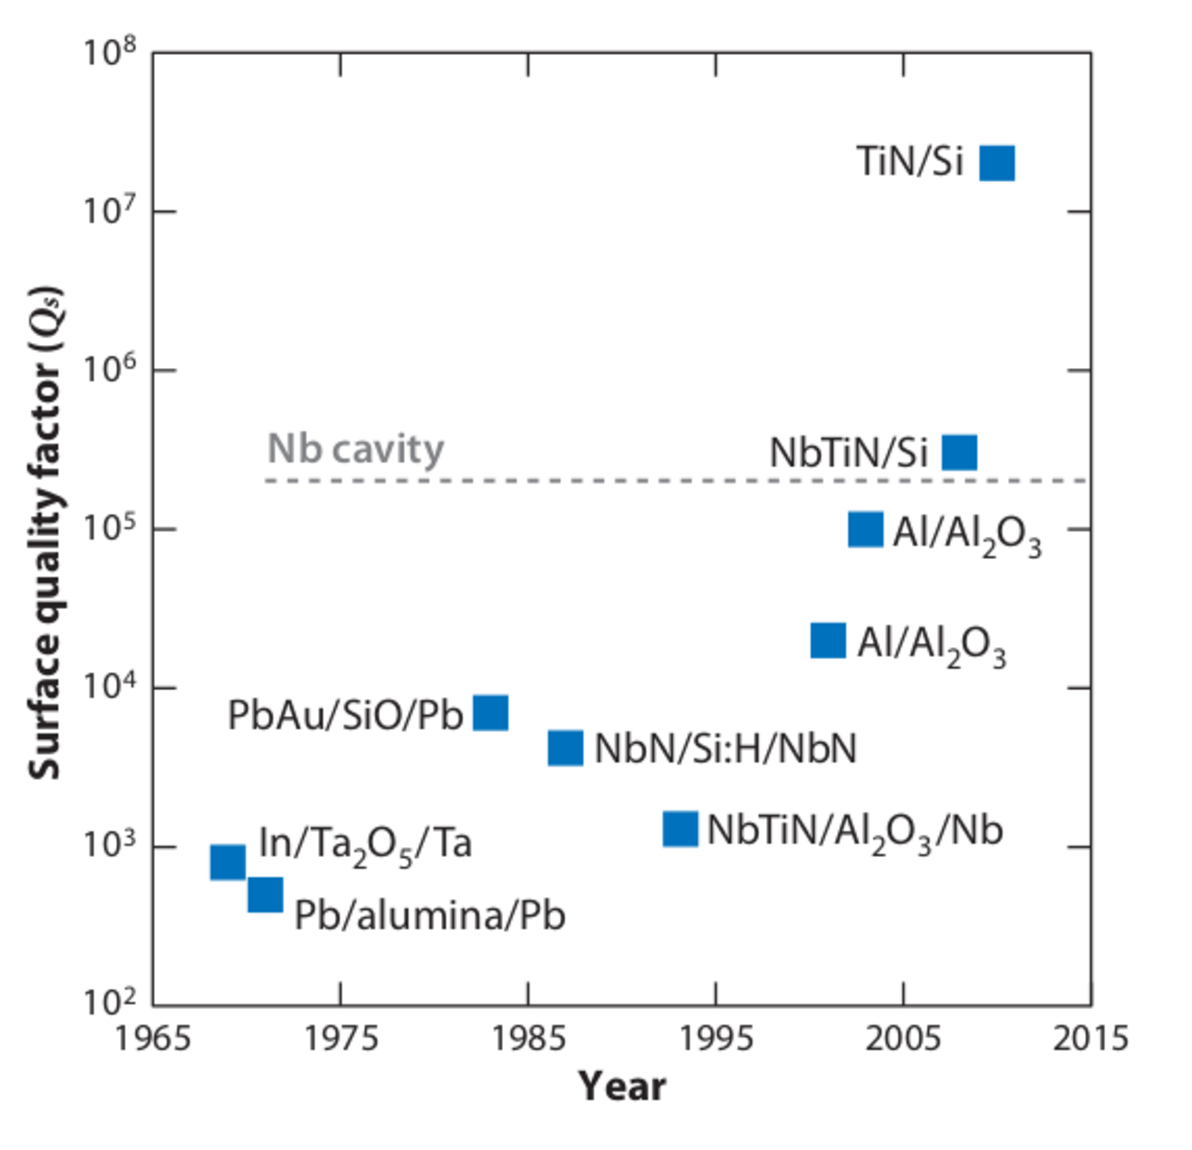
\includegraphics[height=0.68\textheight,width=0.6\textwidth]{microresonadores_sc}
								\end{center}
\end{frame} 

%\begin{frame}
%				\frametitle{Sensor TES}
%								\begin{center}
%												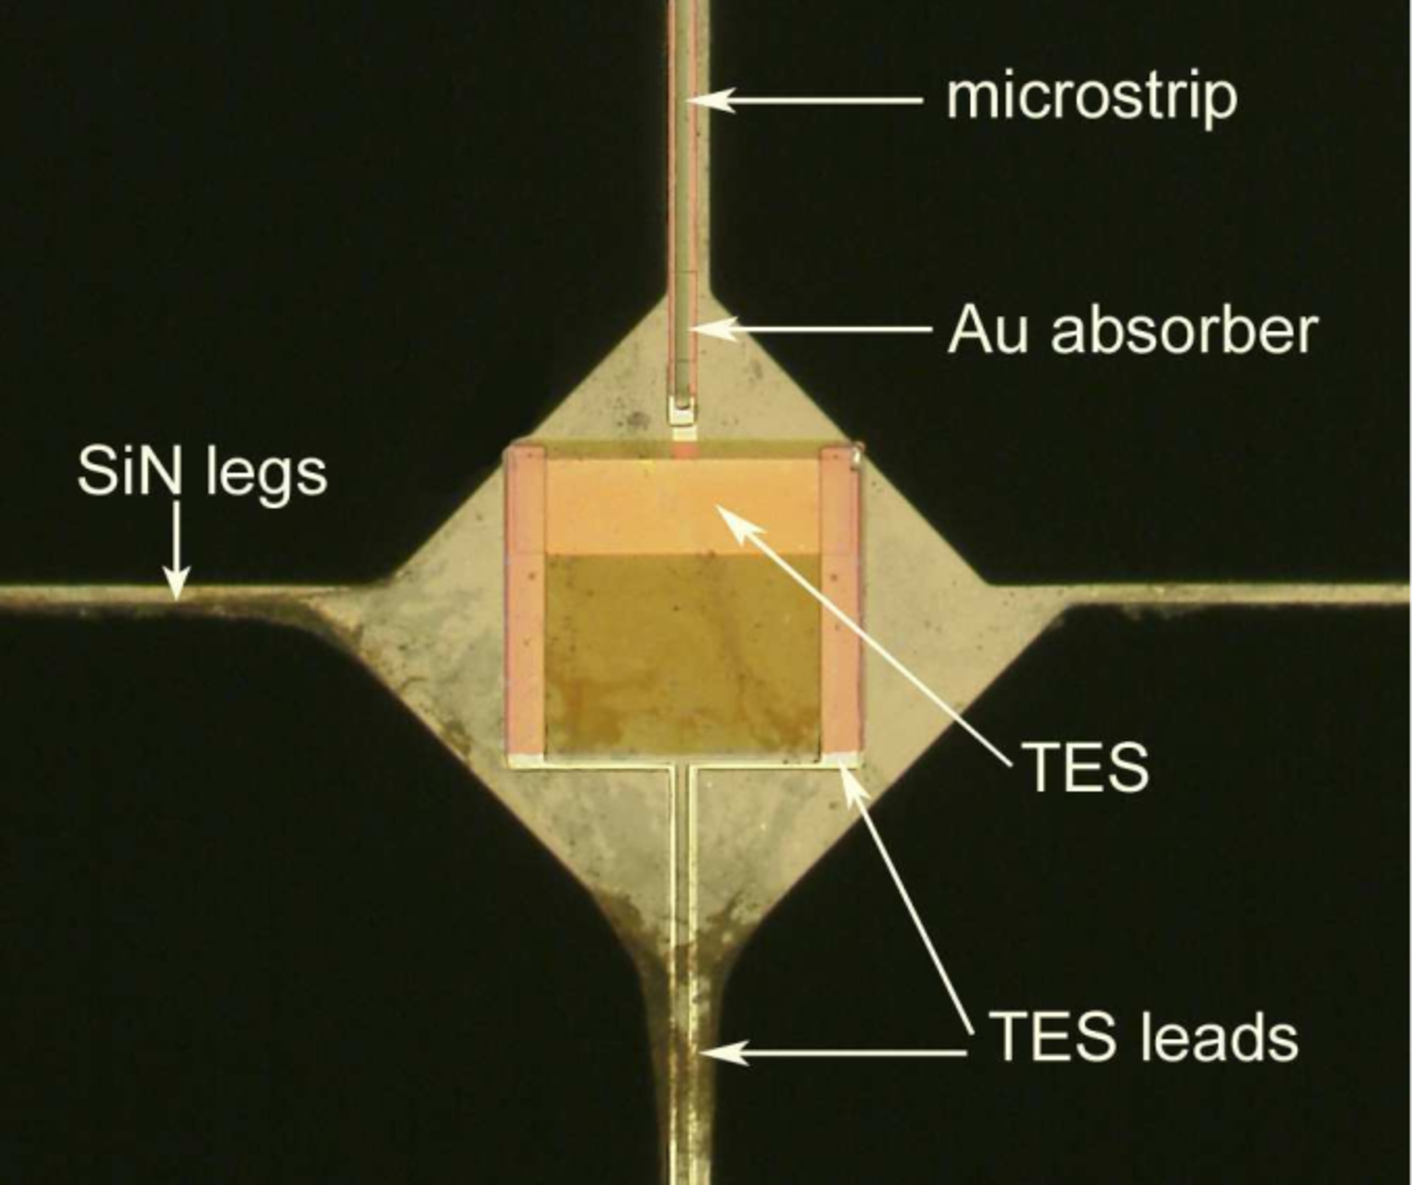
\includegraphics[height=0.68\textheight,width=0.9\textwidth]{sensor_TES}
%								\end{center}
%\end{frame} 

\begin{frame}
				\frametitle{Principales problemas a resolver}
				\begin{itemize}
								\item \alert{No uniformidad de la colección de
												fonones}, especialmente en
								detectores grandes
				\item No uniformidad espacial de la
								recombinación de pares
								electrón-hueco atrapados
								por diversas impurezas
				\item \alert{Ruido} debido a fuentes
								electromagnéticas, especialmente
																microfonía (generación de ruido
																				debido a excitación mecánica,
																acústica y electromagnética)
												\item \alert{Problemas para mantener constante
																la temperatura del bolómetro} y,
												por consiguiente, su \alert{ganancia}
				\end{itemize}
\end{frame}

%\begin{frame}
%				\frametitle{Comparación de resoluciones espacial, en tiempo y en energía
%				de algunos detectores de radiación}
%				%\begin{block}{}
%								\begin{center}
%												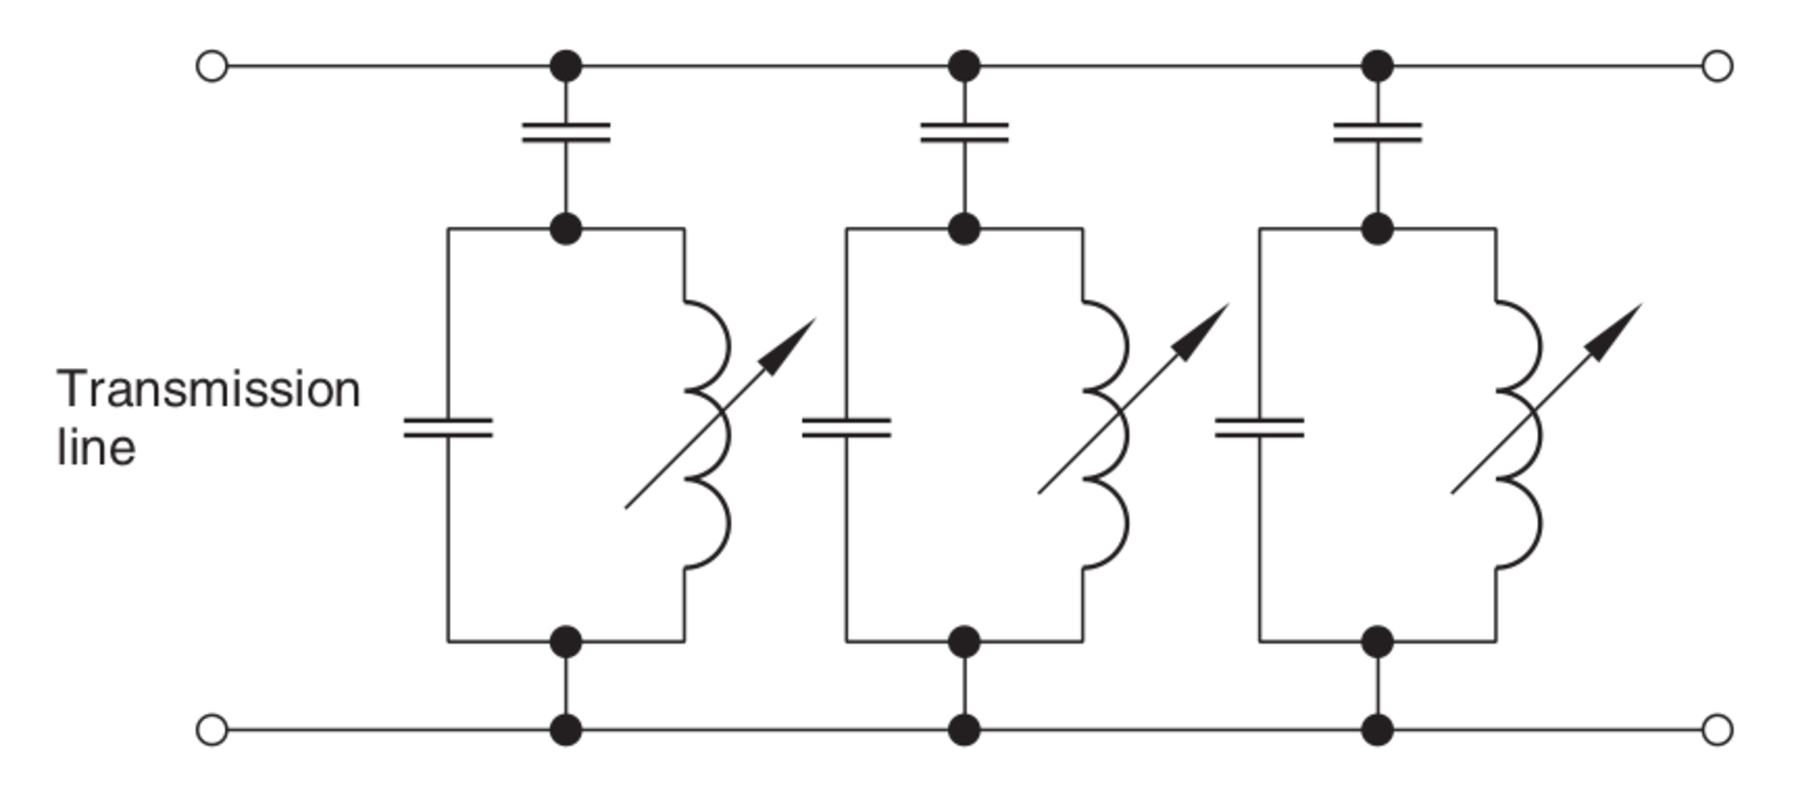
\includegraphics[height=0.68\textheight,width=0.9\textwidth]{esquema_electrico_3_mkids}
%								\end{center}
%								%\end{block}
%\end{frame} 

%------------------------------------------------------------------------------
\section{MKIDs}
%------------------------------------------------------------------------------

\begin{frame}
				\frametitle{Microwave Kinetic Inductance Detectors (MKIDs) y sus usos}
				\begin{columns}
								\begin{column}{0.75\textwidth}
								\begin{block}{}
								\begin{itemize}
								\item Matriz de micro-resonadores pixelado
								\item Detectores superconductores: operados a $<
												300\,\text{mK}$
								\item Sensible a fotones y fonones
												balísticos. Puede proporcionar
												resolución de energía ($
												\Delta E/E$)
												en el espectro visible e
												IR cercano para hacer
												cosmología a gran escala sin
												filtros y etiquetado de fotones
												con resolución de $1\,\mu s$
								\item Al acoplar la inductancia cinética a un
												condensador se obtiene un resonador $\to$ lectura de frecuencia
								\item Construído por foto-litografía
								\item Se puede lograr fácilmente gran integración
				\end{itemize}
\end{block}
\end{column} \ \
				\begin{column}{0.25\textwidth}
				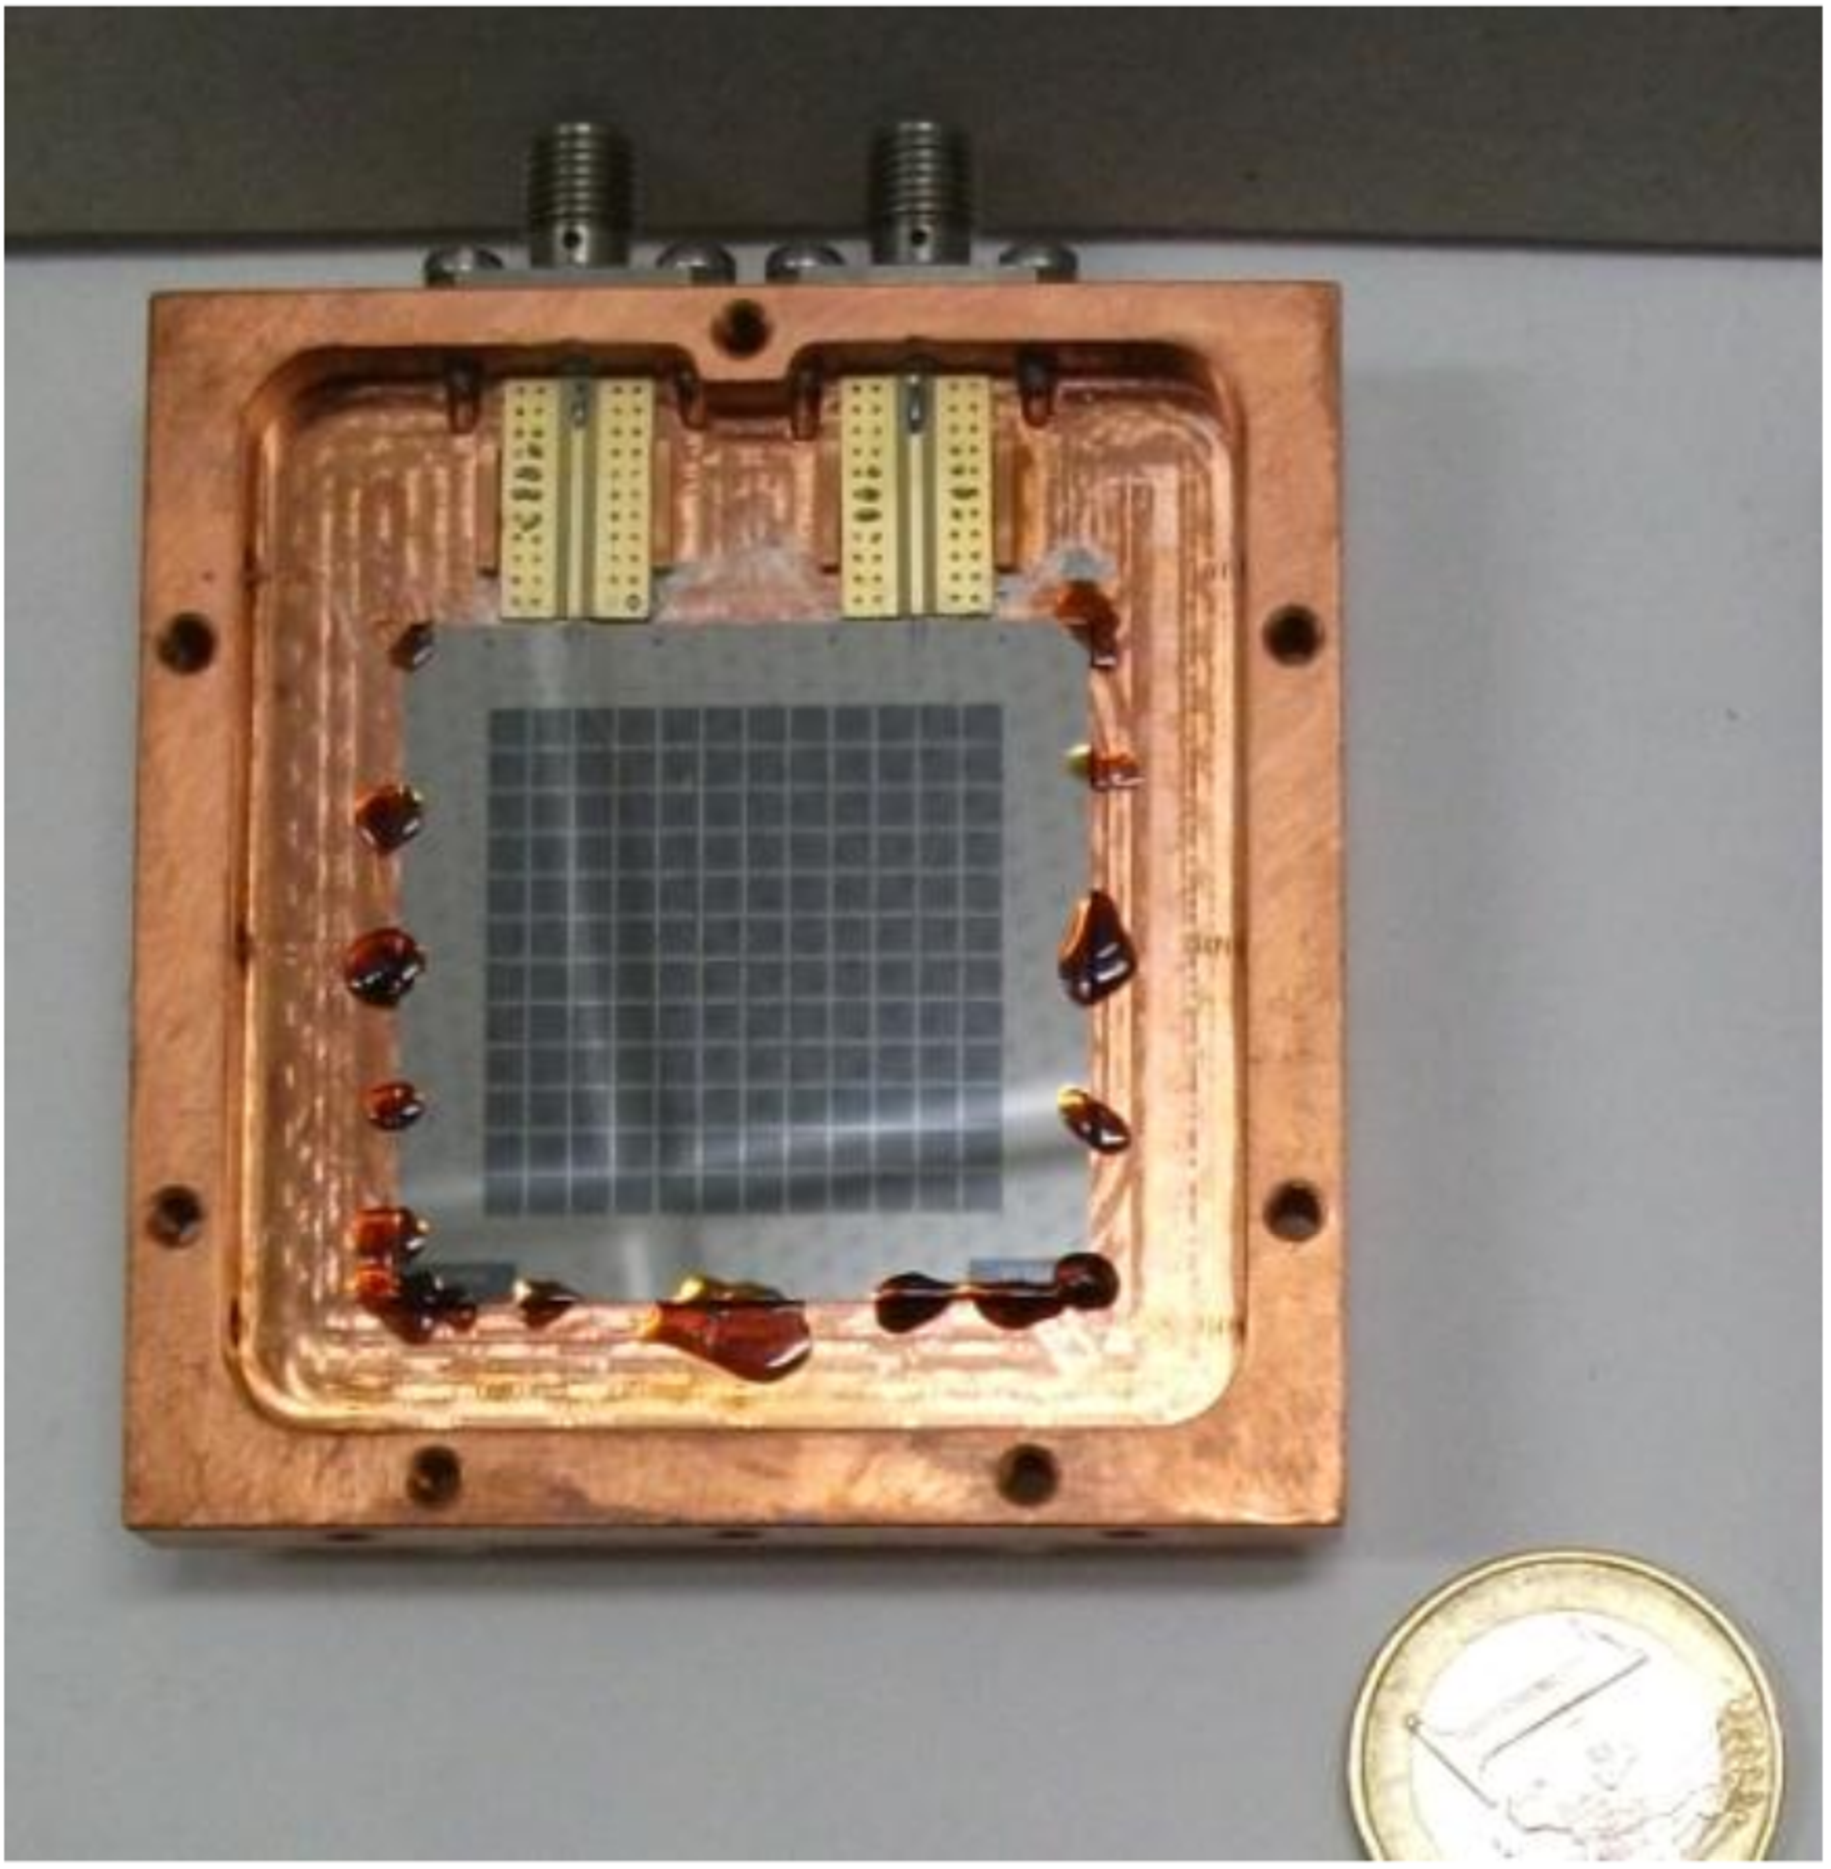
\includegraphics[width=0.8\textwidth]{arreglo_mkid_144px}
				Arreglo de 144 píxeles
\end{column}
\end{columns}
\end{frame}

\begin{frame}
\frametitle{Microwave Kinetic Inductance Detectors (MKIDs) y sus usos
(cont.)}
\begin{columns}
\begin{column}{0.55\textwidth}
%								\begin{block}{}
\begin{alertblock}{Aplicaciones}
\begin{itemize}
\item Detección mediada por \textbf{fotones}: detector
				para astronomía en $\lambda \sim \text{mm}$, rayos X, ...
\item Detección mediada por \textbf{fonones}:
\begin{itemize}
				\item Detector de partículas (rayos cósmicos, detección de materia oscura, ...)
				\item Herramienta para caracterizar la propagación de fonones en diversos materiales
												\end{itemize}
				\end{itemize}
				\end{alertblock}
				%								\end{block}
\end{column} \ \
\begin{column}{0.45\textwidth}
				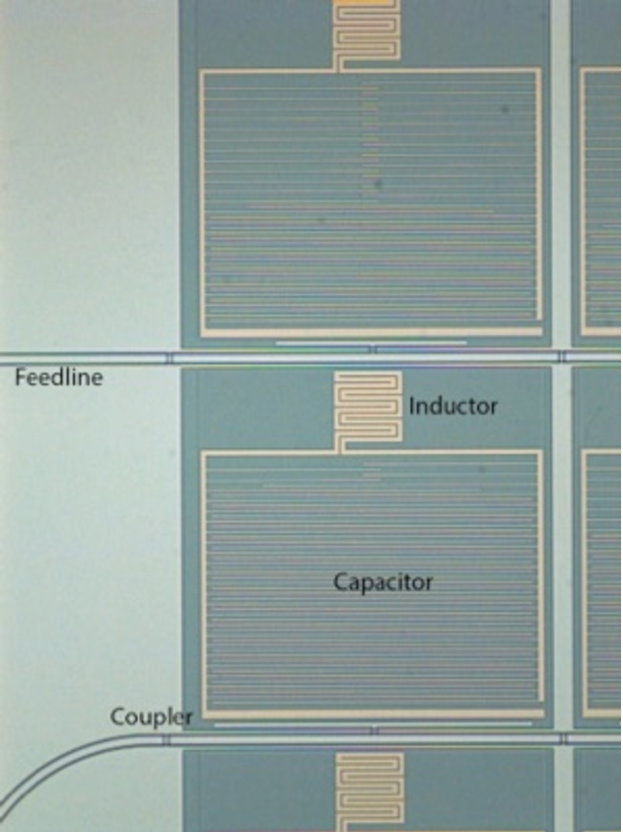
\includegraphics[width=0.8\textwidth]{otra_foto_mkid_mazin}
								\end{column}
				\end{columns}

\end{frame}

\begin{frame}
				\frametitle{MKID: principio de funcionamiento}
				%\begin{block}{}
								\begin{center}
												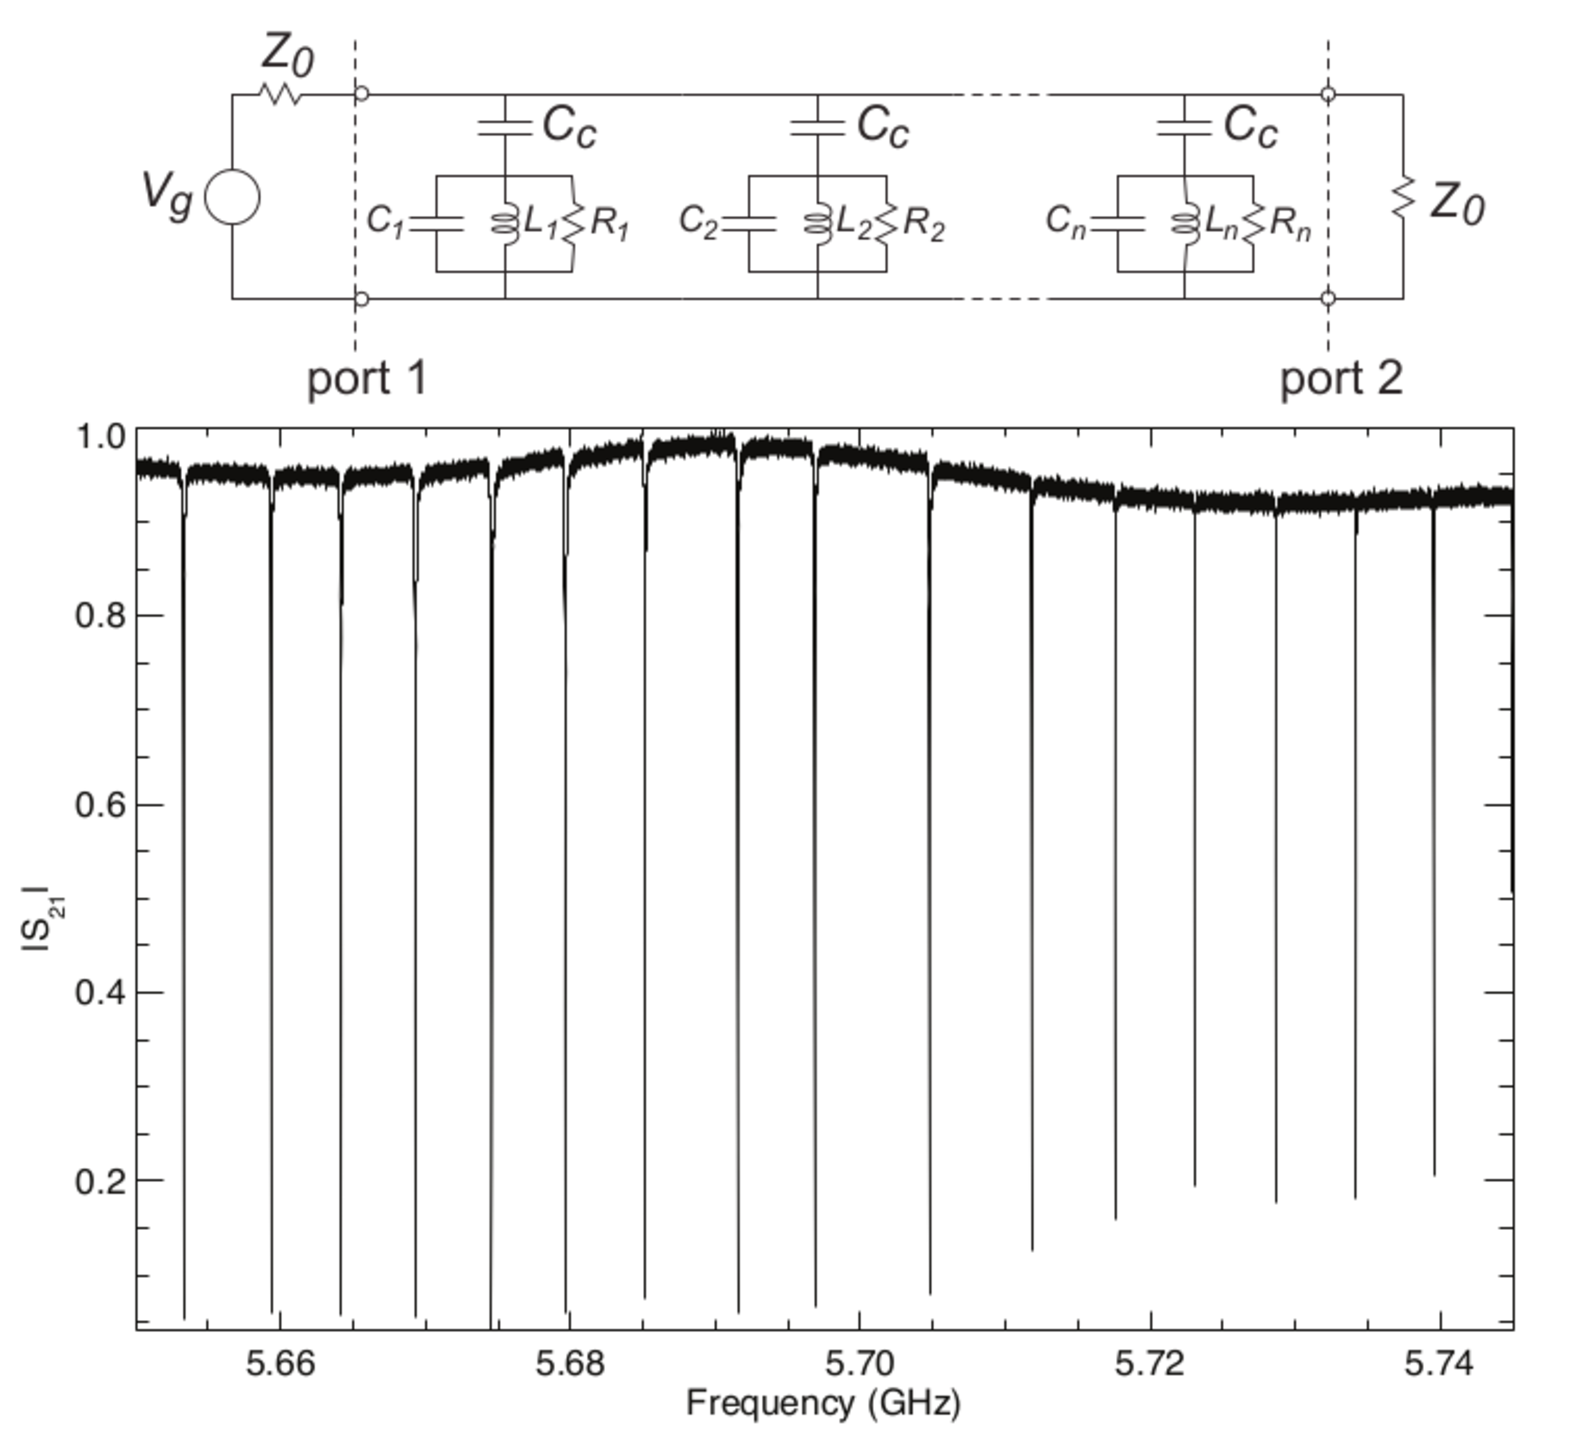
\includegraphics[height=0.68\textheight,width=0.8\textwidth]{circuito_equiv_y_transmision}
												%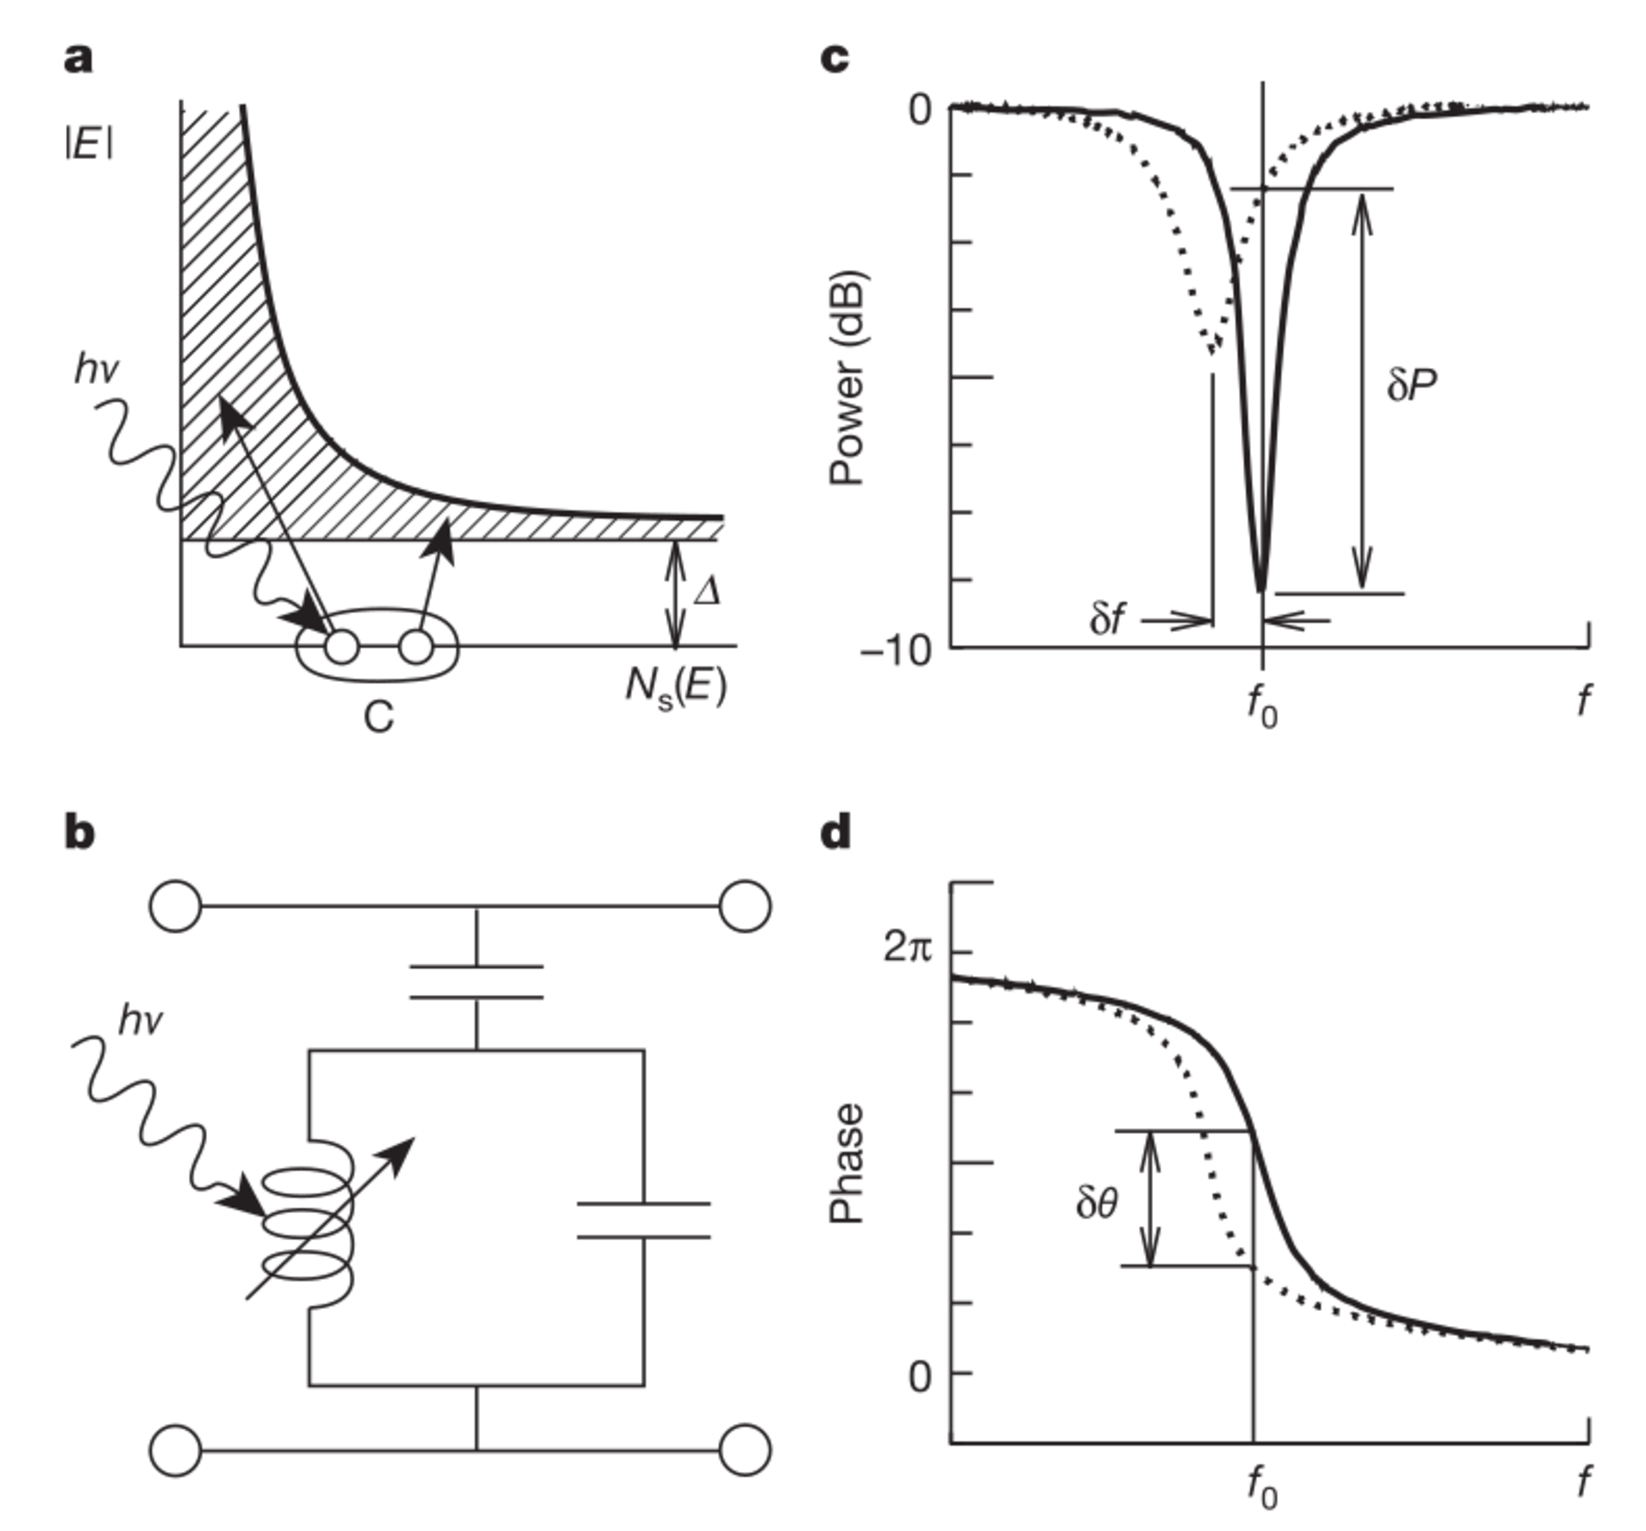
\includegraphics[height=0.68\textheight,width=0.9\textwidth]{principio_mkid}
								\end{center}
								%\end{block}
\end{frame} 

\begin{frame}
\frametitle{MKID: principio de funcionamiento}
%\begin{block}{}
				\begin{center}
								\only<1>{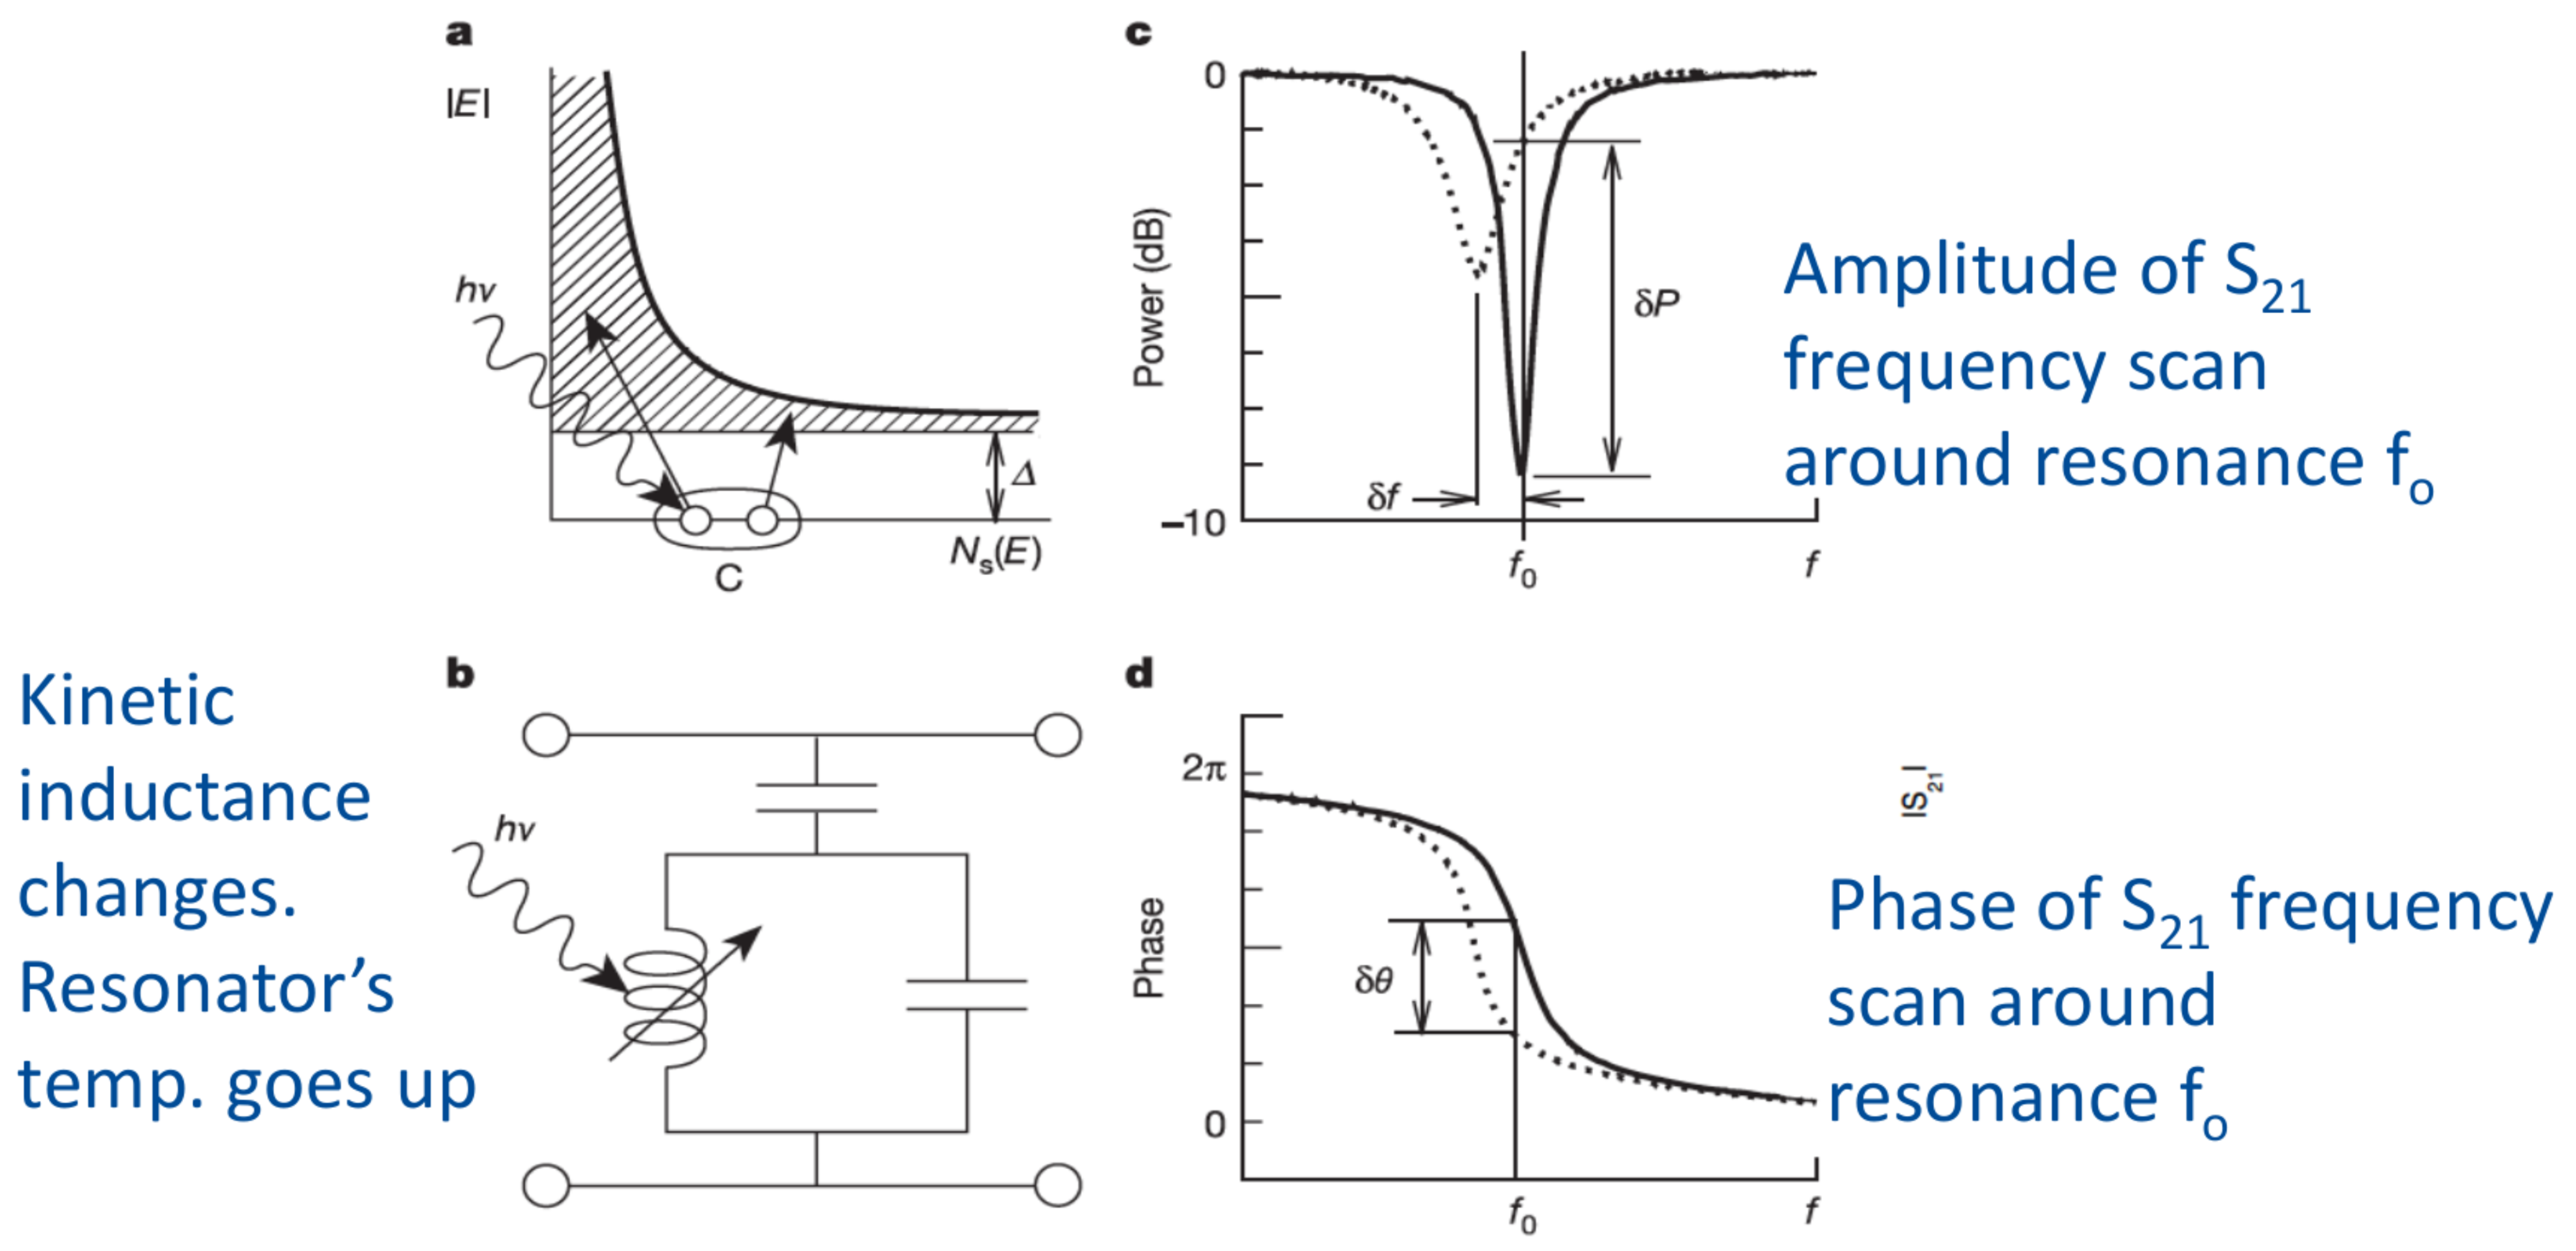
\includegraphics[height=0.58\textheight,width=0.9\textwidth]{principio_mkid_gustavo}}
								\only<2>{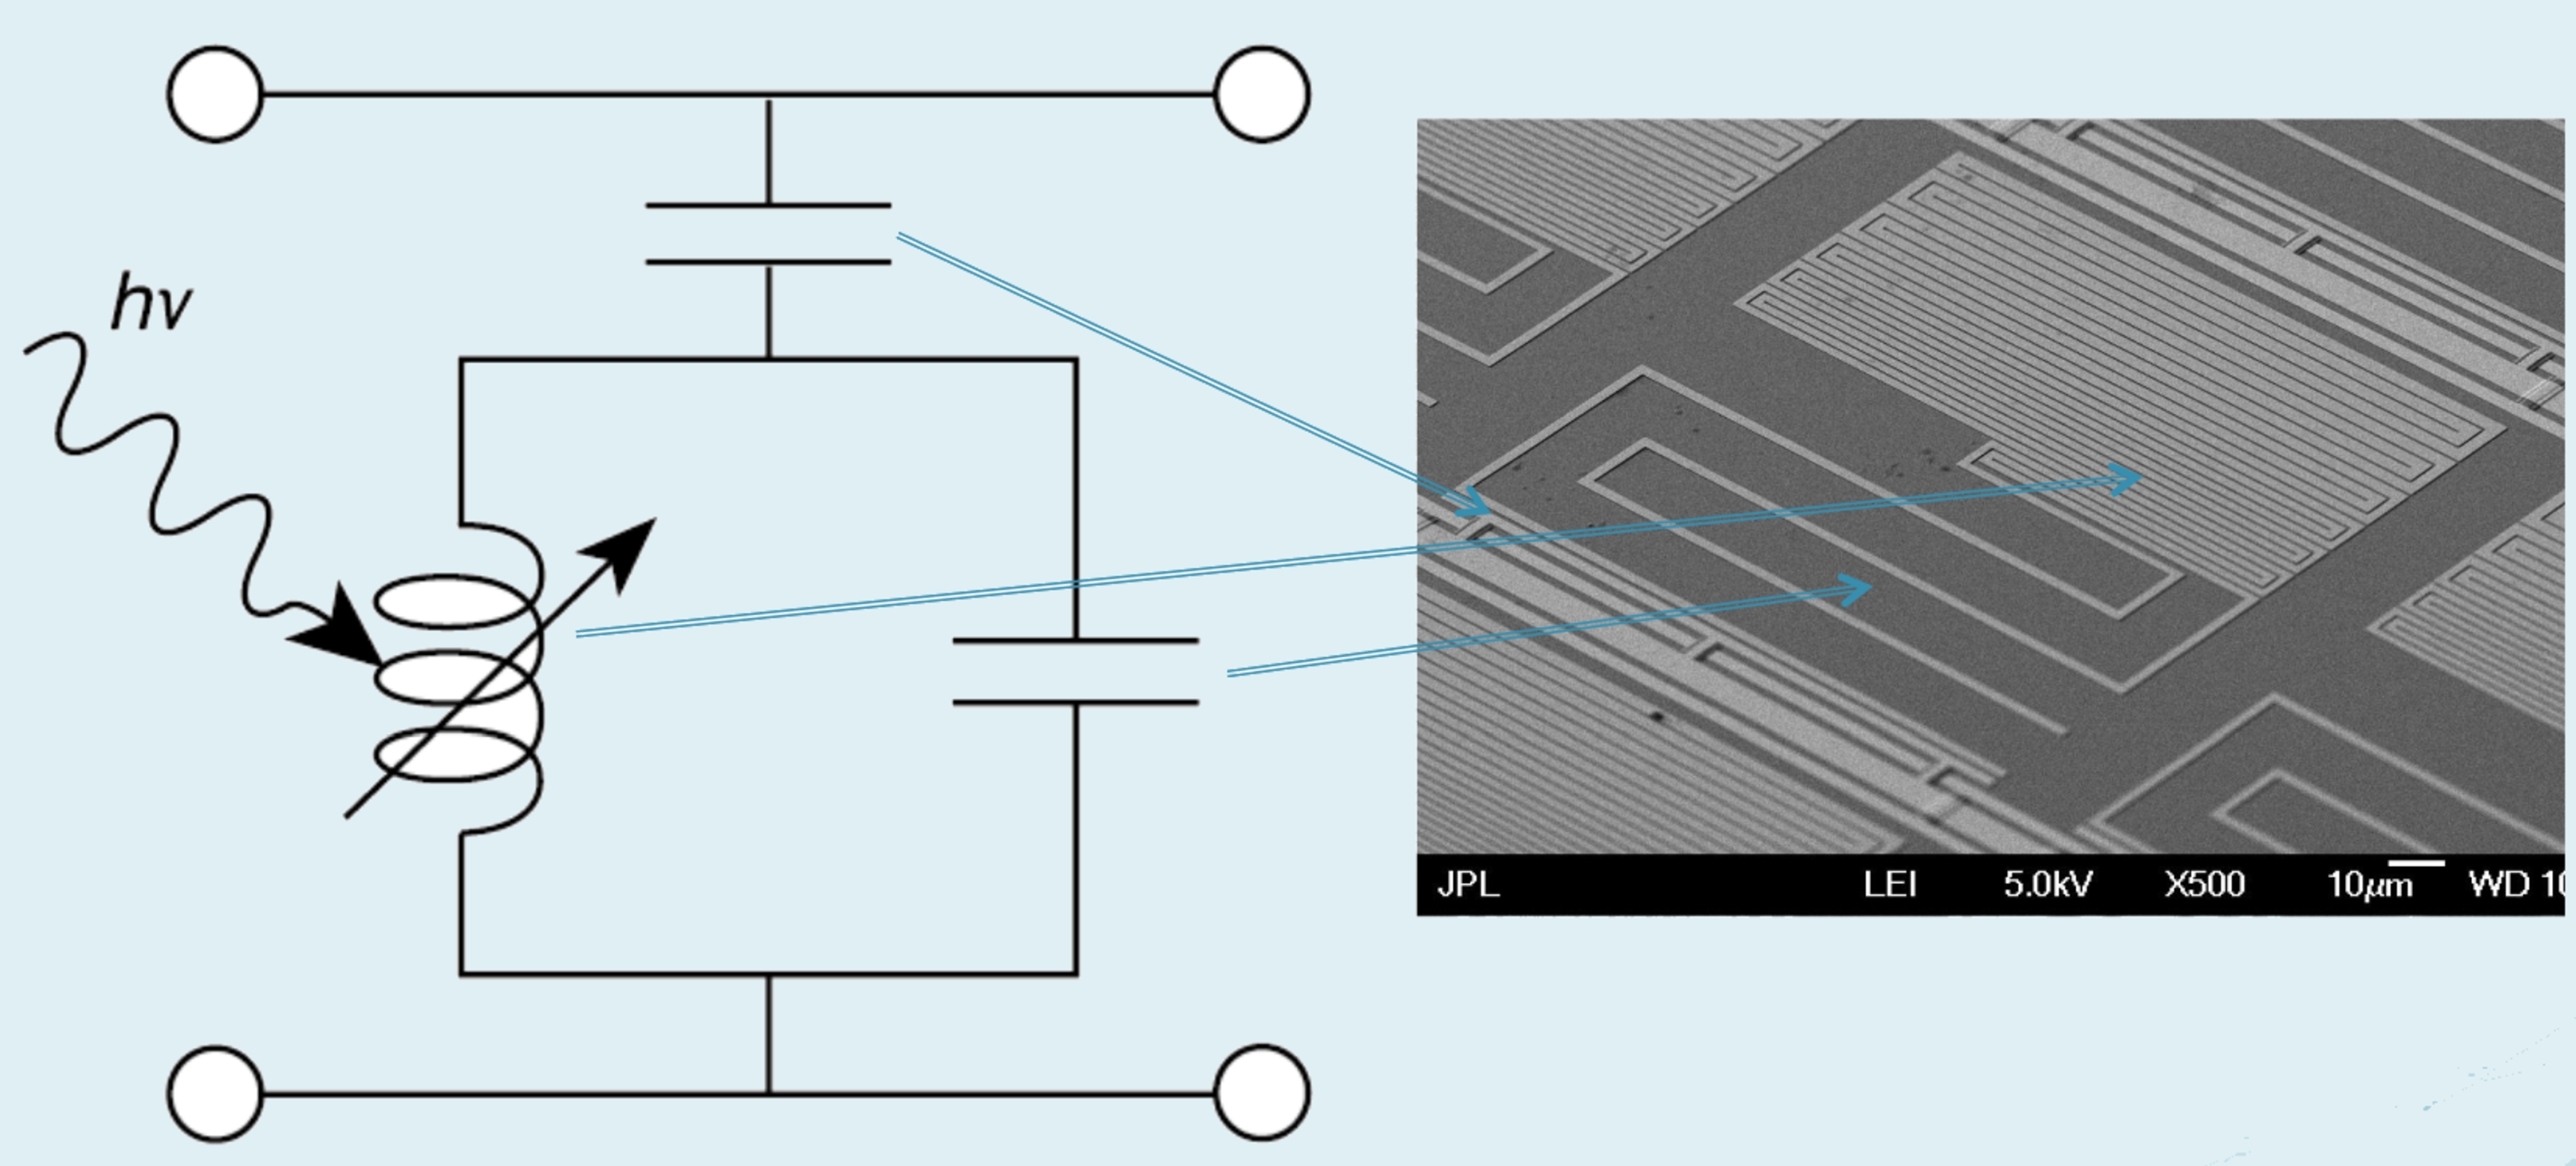
\includegraphics[height=0.58\textheight,width=0.9\textwidth]{equiv_mkid_sustrato}}
				\end{center}
																				\begin{itemize}
\item Los fotones alcanzan un píxel y mueven la resonancia de ese píxel
\item Se mide la
								dinámica de la
																				señal de fase/amplitud
				\end{itemize}
				%\end{block}
\end{frame} 

\begin{frame}
\frametitle{MKID: principio de funcionamiento}
Energy gap:\\
Silicio --  1.10000 eV\\
Aluminio -- 0.00018 eV
%\begin{block}{}
								\begin{columns}
												\begin{column}{0.5\textwidth}
																\begin{center}
																				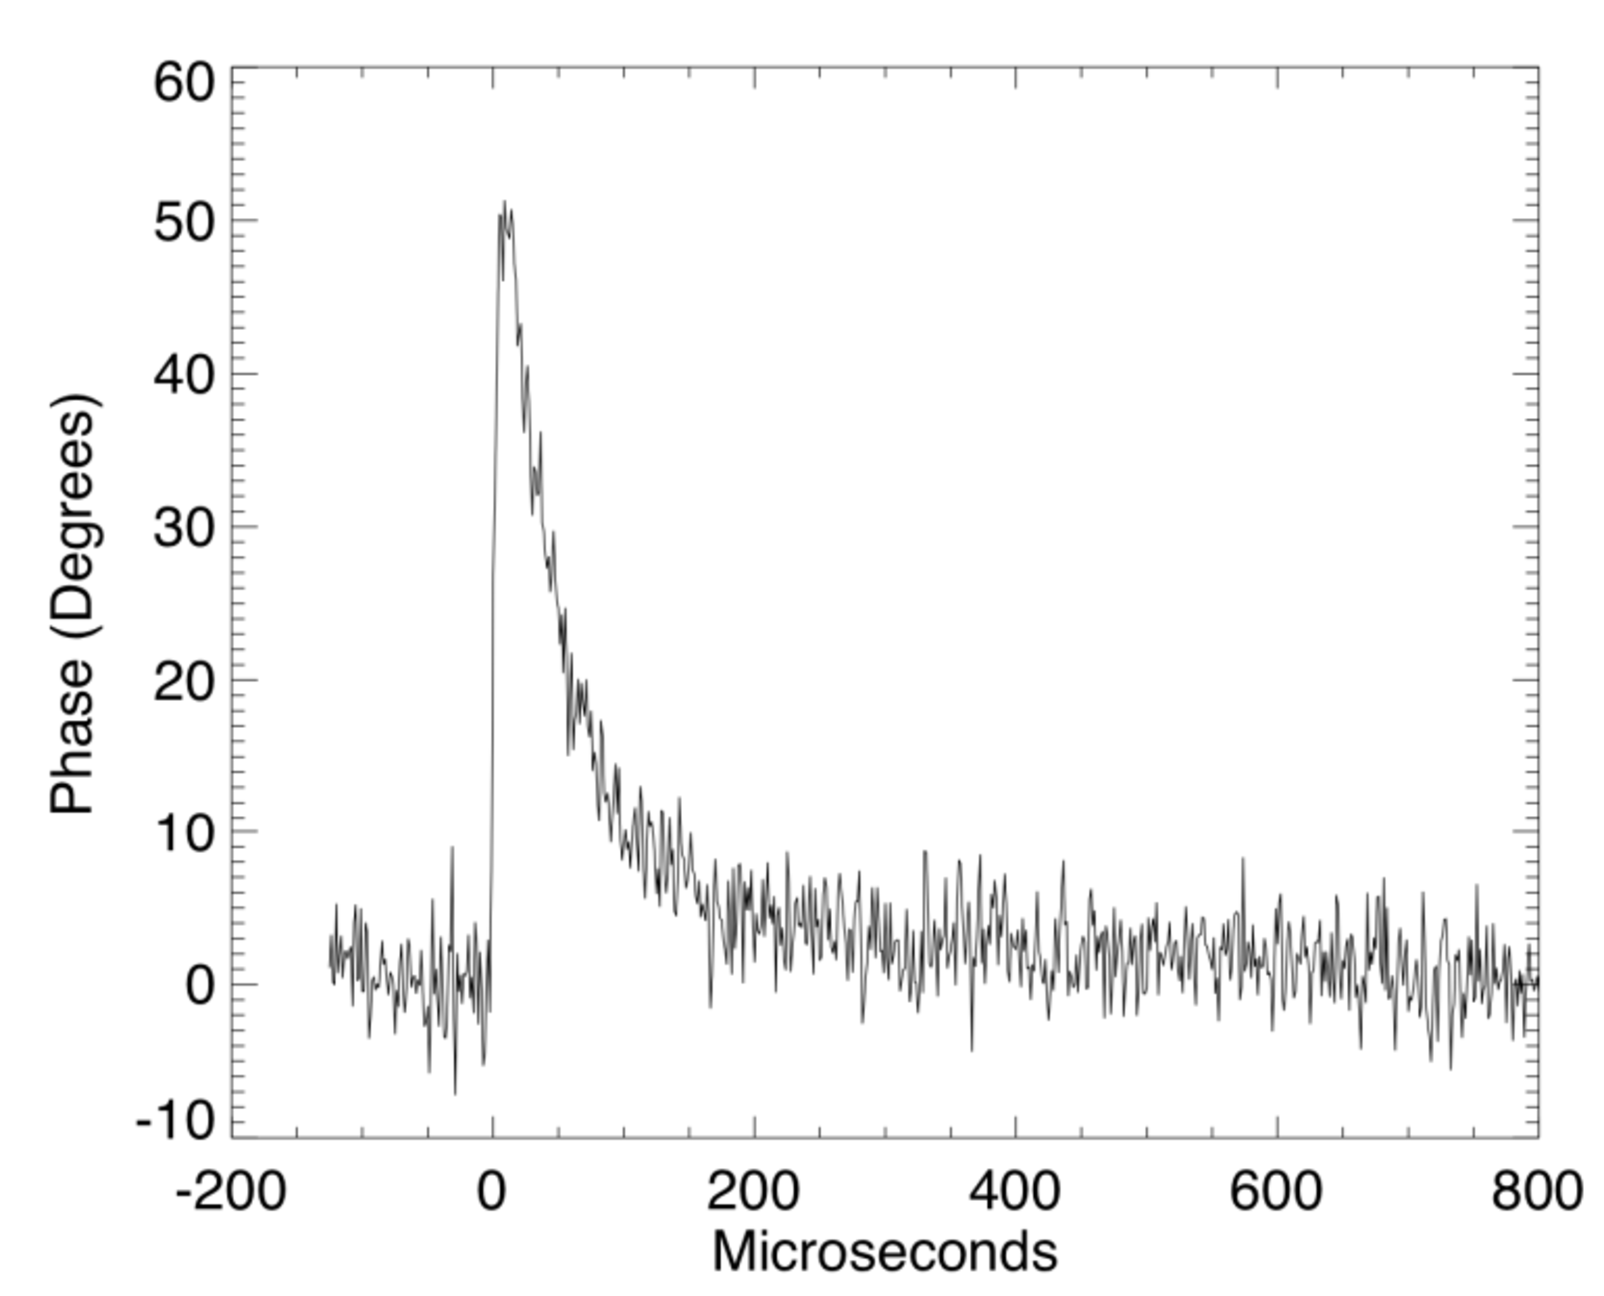
\includegraphics[height=0.54\textheight,width=0.9\textwidth]{evento_mkid1}
																\end{center}
												\end{column}
												\begin{column}{0.5\textwidth}
																\begin{center}
																				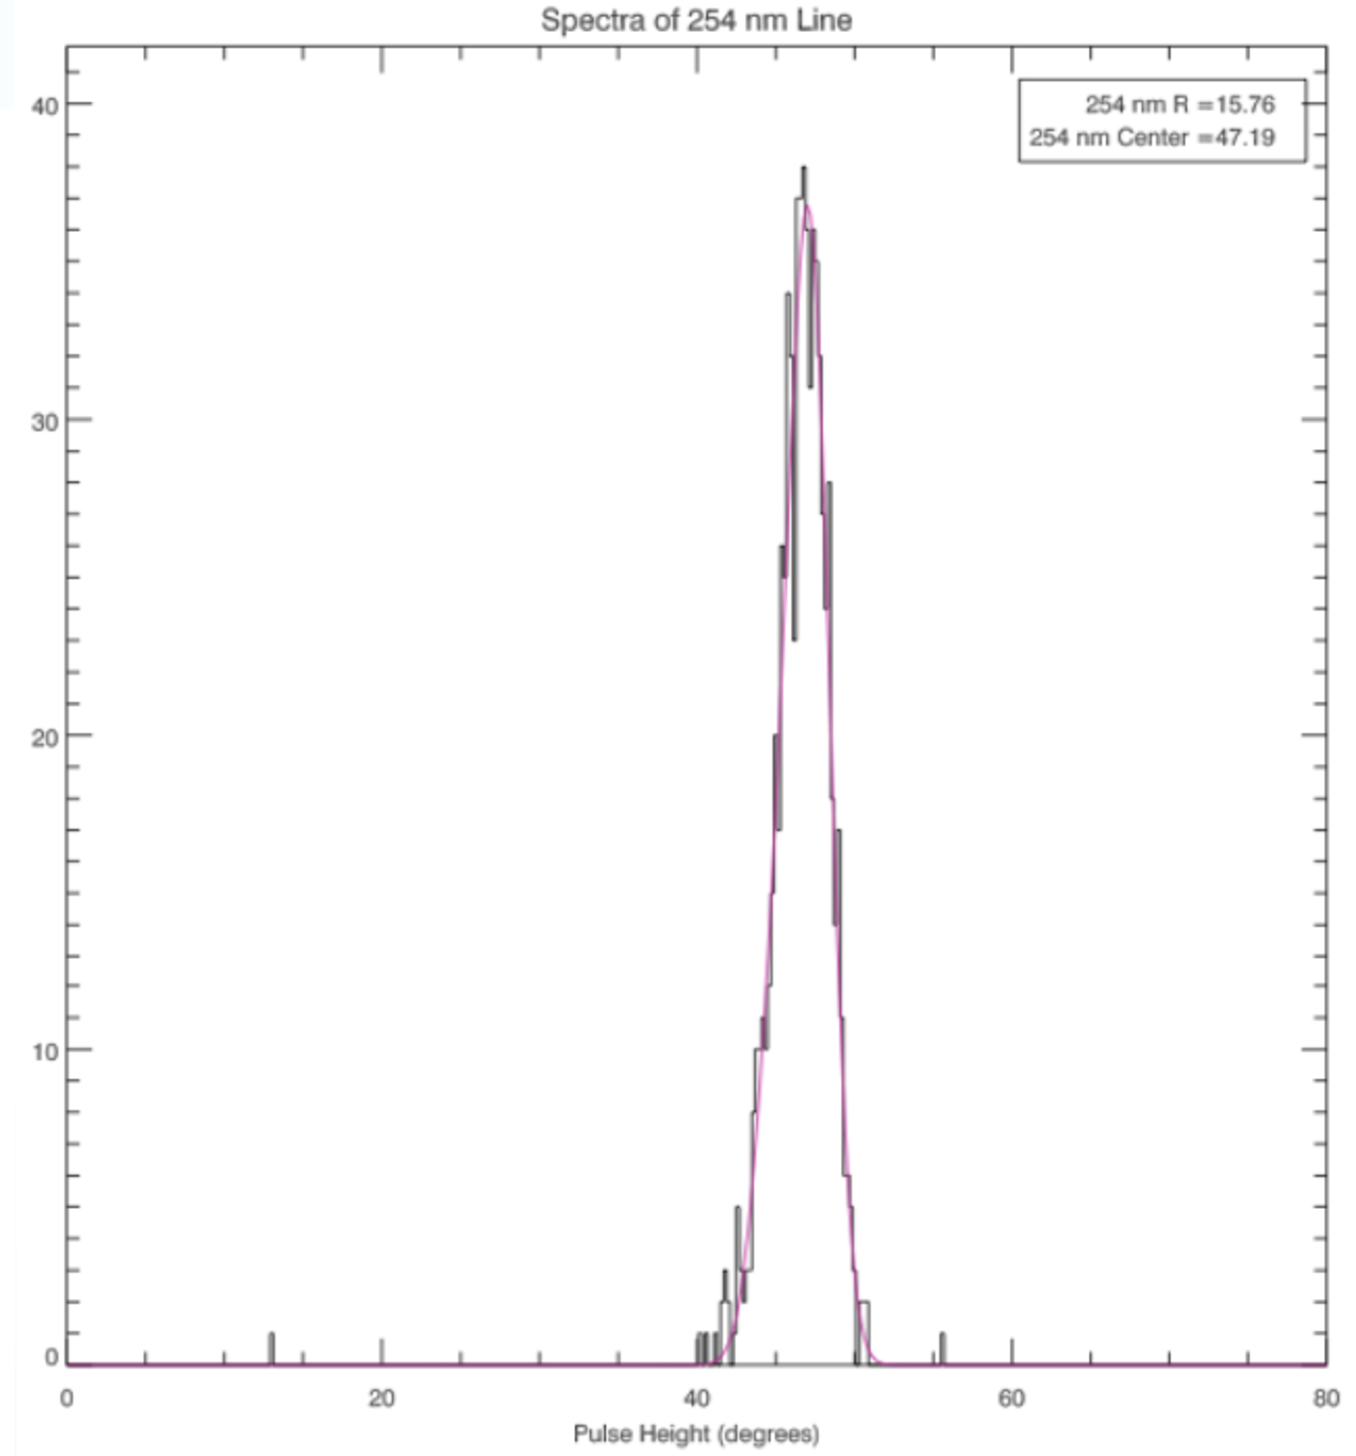
\includegraphics[height=0.54\textheight,width=0.9\textwidth]{evento_mkid2}
																\end{center}
												\end{column}
								\end{columns}

				\end{frame} 

				\begin{frame}
								\frametitle{Método de instrumentación del arreglo}
								\begin{itemize}
																%				\pause
												\item[*] Excitación: generación de un peine de
																frecuencias (\alert{FDM}):
																\begin{itemize}
																				\item Contiene el mayor número posible de frecuencias
																				\item Cada frecuencia ajustable a una resolución de kHz
																				\item Cada tono generado en la versión
																								en fase (I) y en cuadratura (Q)
																\end{itemize}

												\item[*] Conversión ascendente (up-conversion) del peine de frecuencia generado en banda base
												\item[*] La señal pasa a través de la matriz y finalmente se modifica
												\item[*] En la salida de la matriz, conversión
																descendente (down-conversion) a banda base
												\item[*] Procesamiento de señal: determina cada fase y
																amplitud de los tonos
								\end{itemize}
								%\begin{block}{}
												\begin{center}
																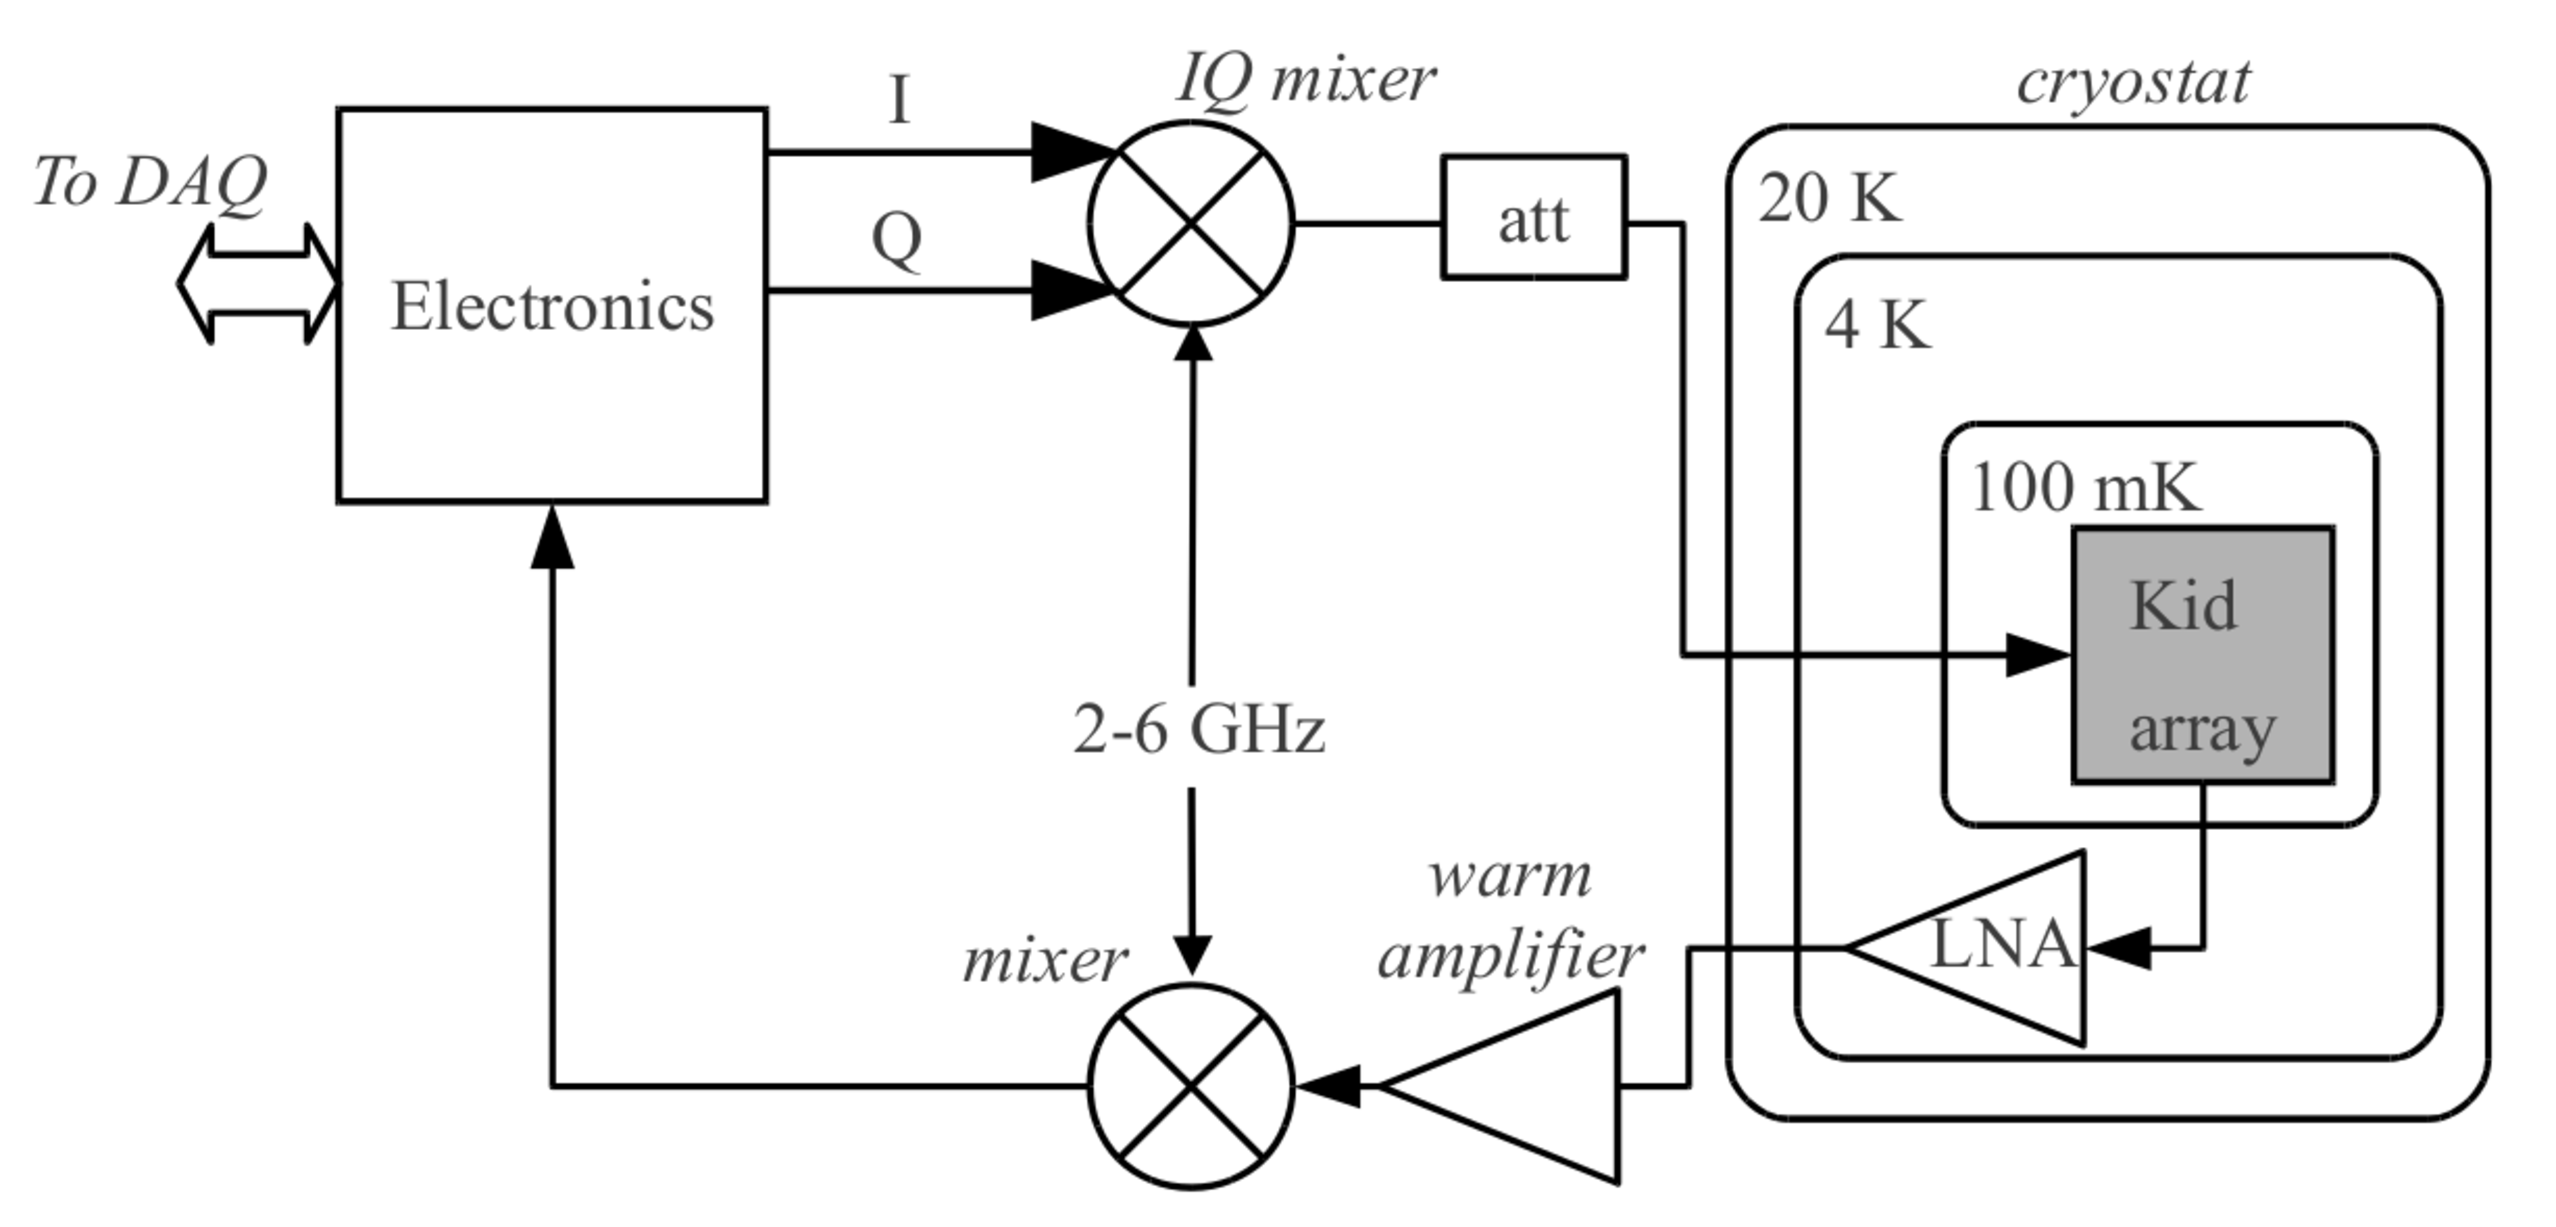
\includegraphics[height=0.3\textheight,width=0.4\textwidth]{mkid_readout}
												\end{center}
												%\end{block}
				\end{frame} 

				%------------------------------------------------------------------------------
				%\subsection{Método de instrumentación del arreglo}
				%------------------------------------------------------------------------------

\begin{frame}
\frametitle{Materiales utilizados}
\begin{center}
				\only<1>{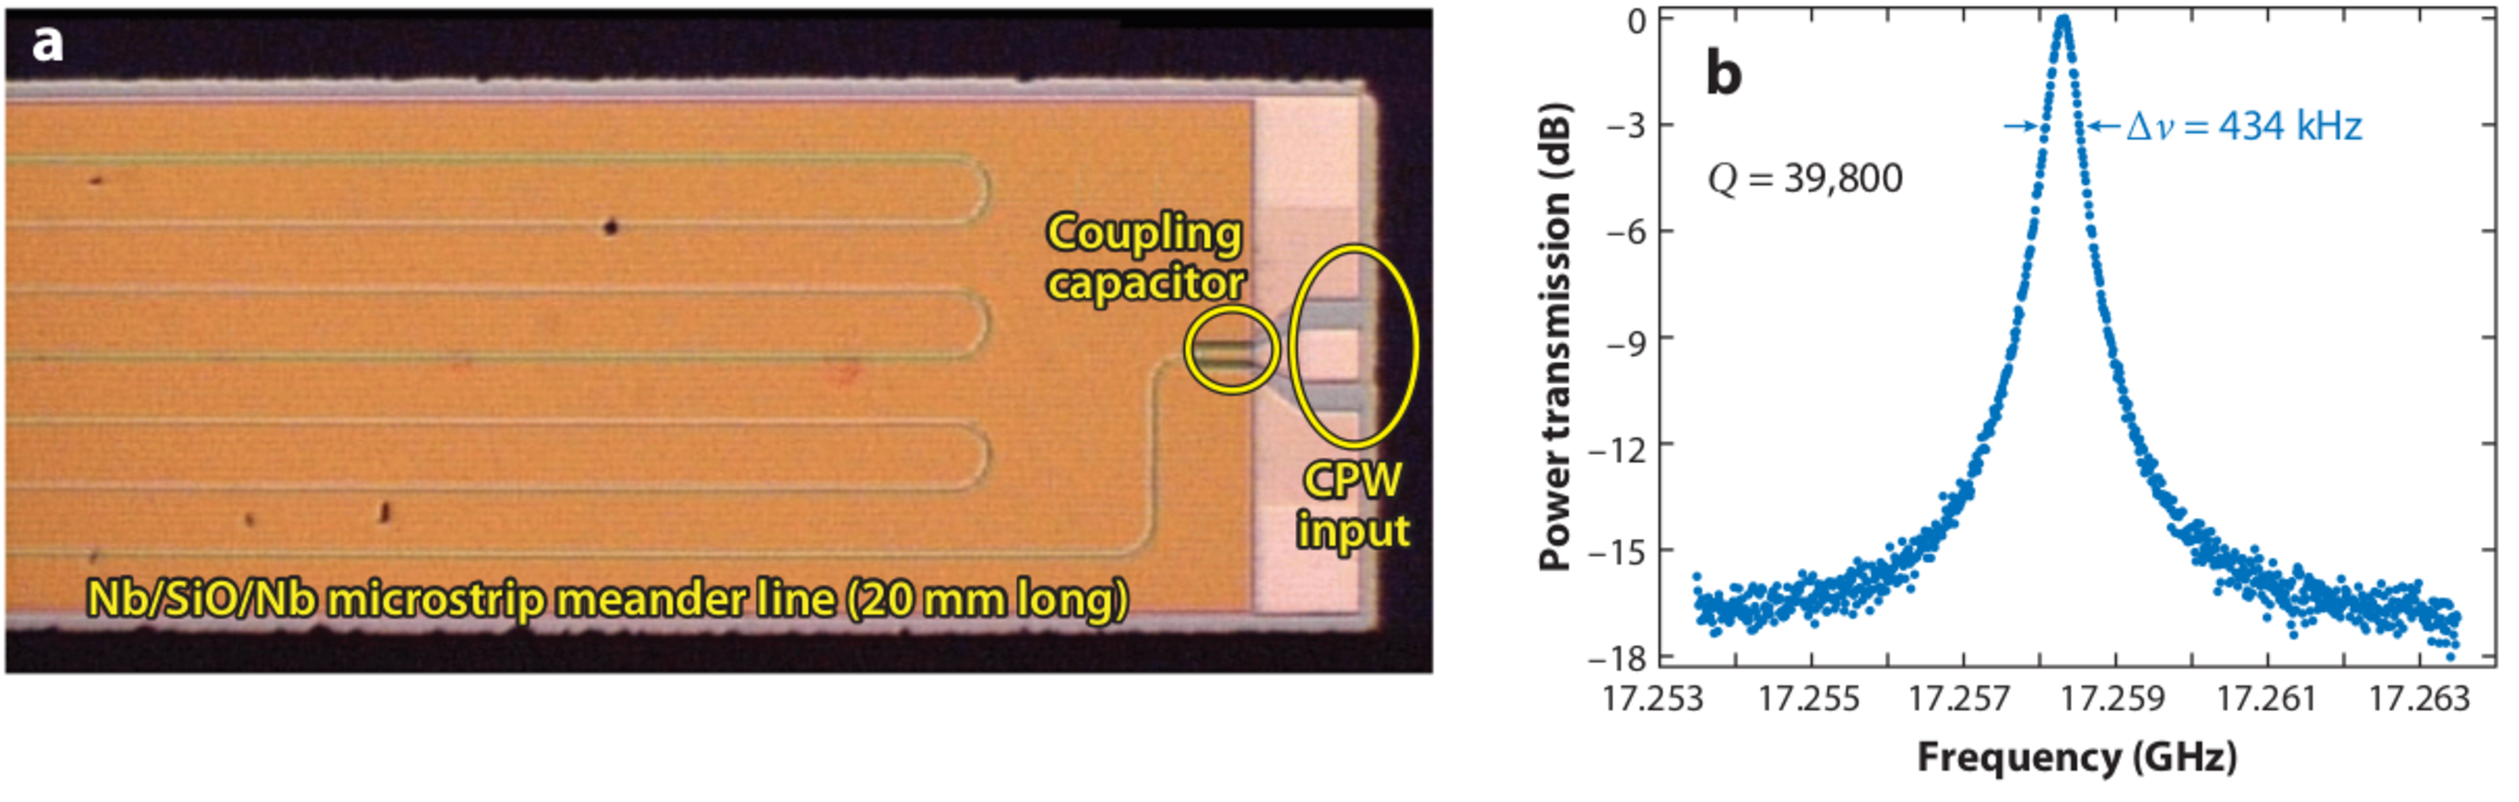
\includegraphics[height=0.5\textheight,width=0.9\textwidth]{NbSiONb_mkid}}
\end{center}
				\only<1>{Resonador microstrip de \alert{$\lambda / 2$}
				hecho de  \alert{$Nb/SiO/Nb$}. El capacitor de
acoplamiento es una estructura de placa
paralela de $Nb/SiO/Nb$ y resultados de medición a
				\alert{17.26 GHz} con una potencia de microondas
				relativamente alta, mostrando \alert{$Q_r = 4 \times
								10^4$}} 
								%Esta resonancia es el sexto armónico de la
								%				resonancia fundamental de 2.86 GHz.}
\begin{columns}
\begin{column}{0.5\textwidth}
\begin{itemize}
\item<3> \tiny{Resonadores
				(microstrip) de\\
				\alert{$In/Ta_2 O_5/Ta$}\\
				\alert{$Nb/SiO/Nb$}\\ 
				\alert{$PbAu/SiO/Pb$}\\ 
				\alert{$NbN/Si:H/NbN$}\\ 
				\alert{$NbTiN$}\\
				\alert{$NiT$}} 
								\only<3>{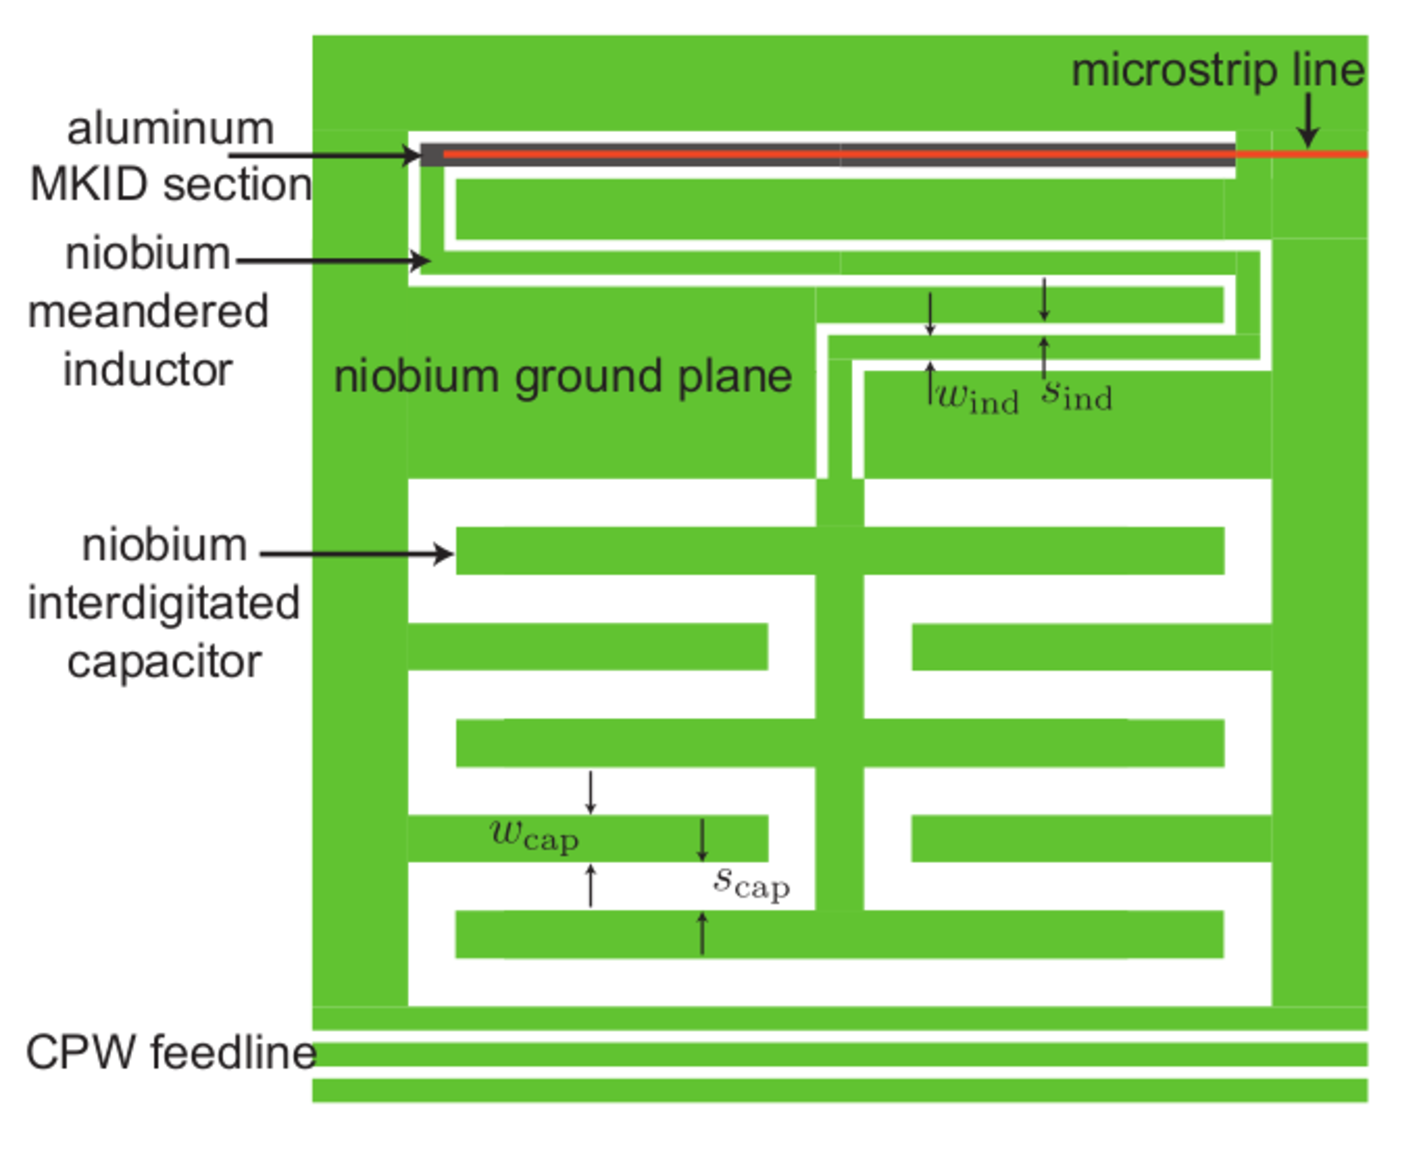
\includegraphics[height=0.48\textheight,width=0.8\textwidth]{mkid_de_noroozian}}
								\item<2> Resonadores de \alert{Al} sobre
																zafiro y capa de \alert{$Si
																N_x$}
								\end{itemize}
				\end{column}
				\begin{column}{0.5\textwidth}
				\begin{center}
								\only<3>{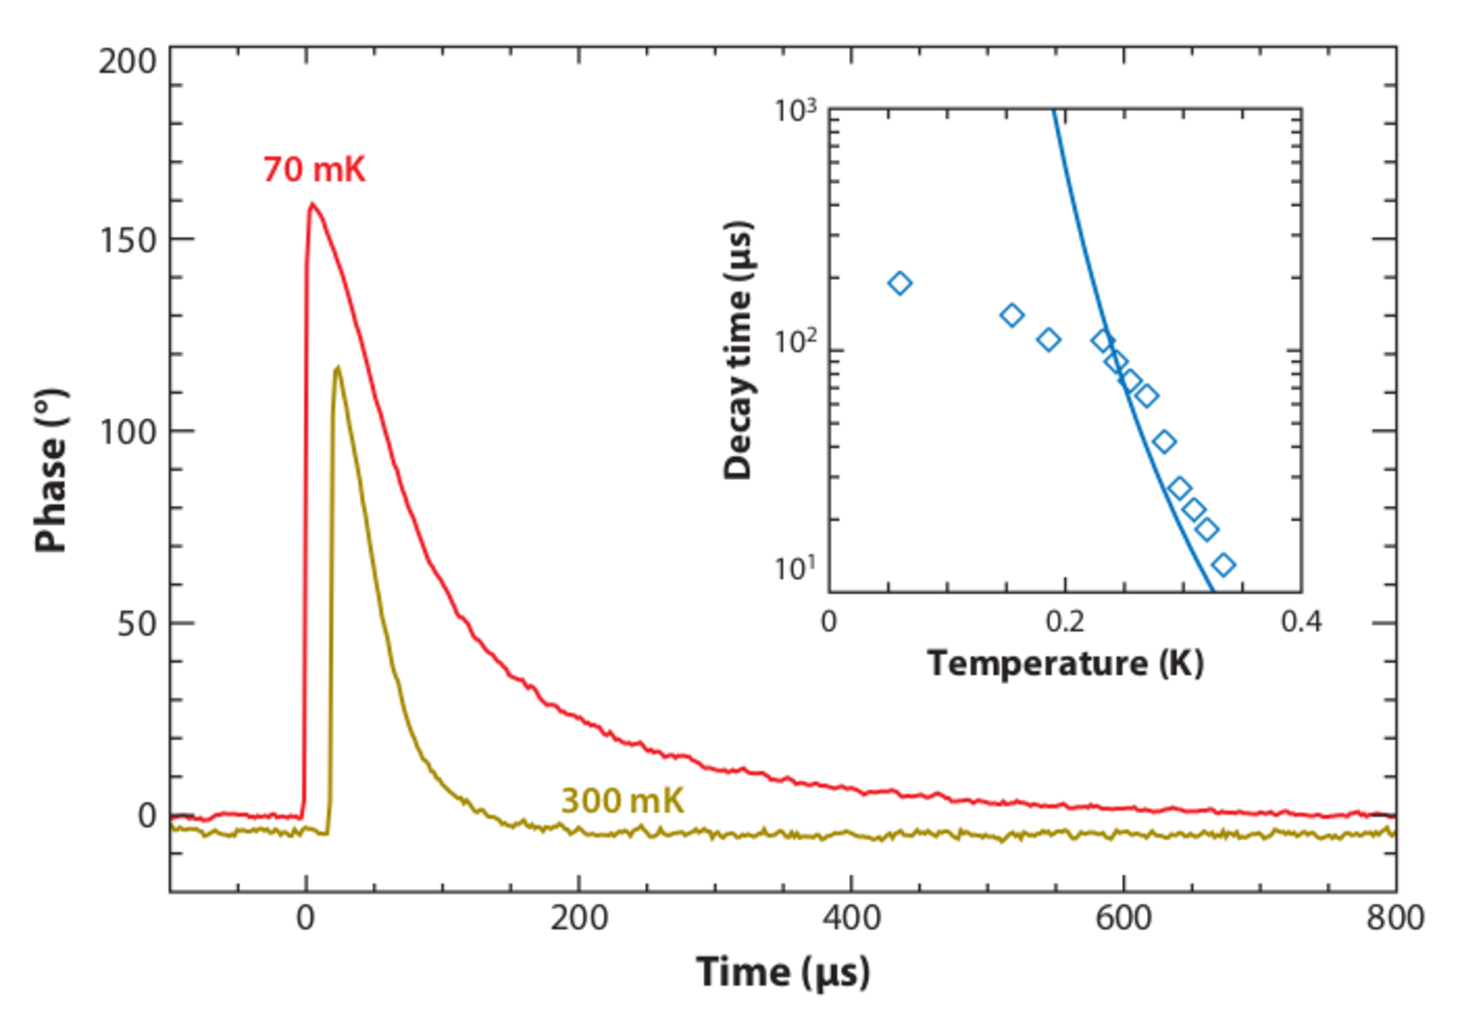
\includegraphics[height=0.44\textheight,width=0.8\textwidth]{respuesta_mkid_con_T}}
												\only<2>{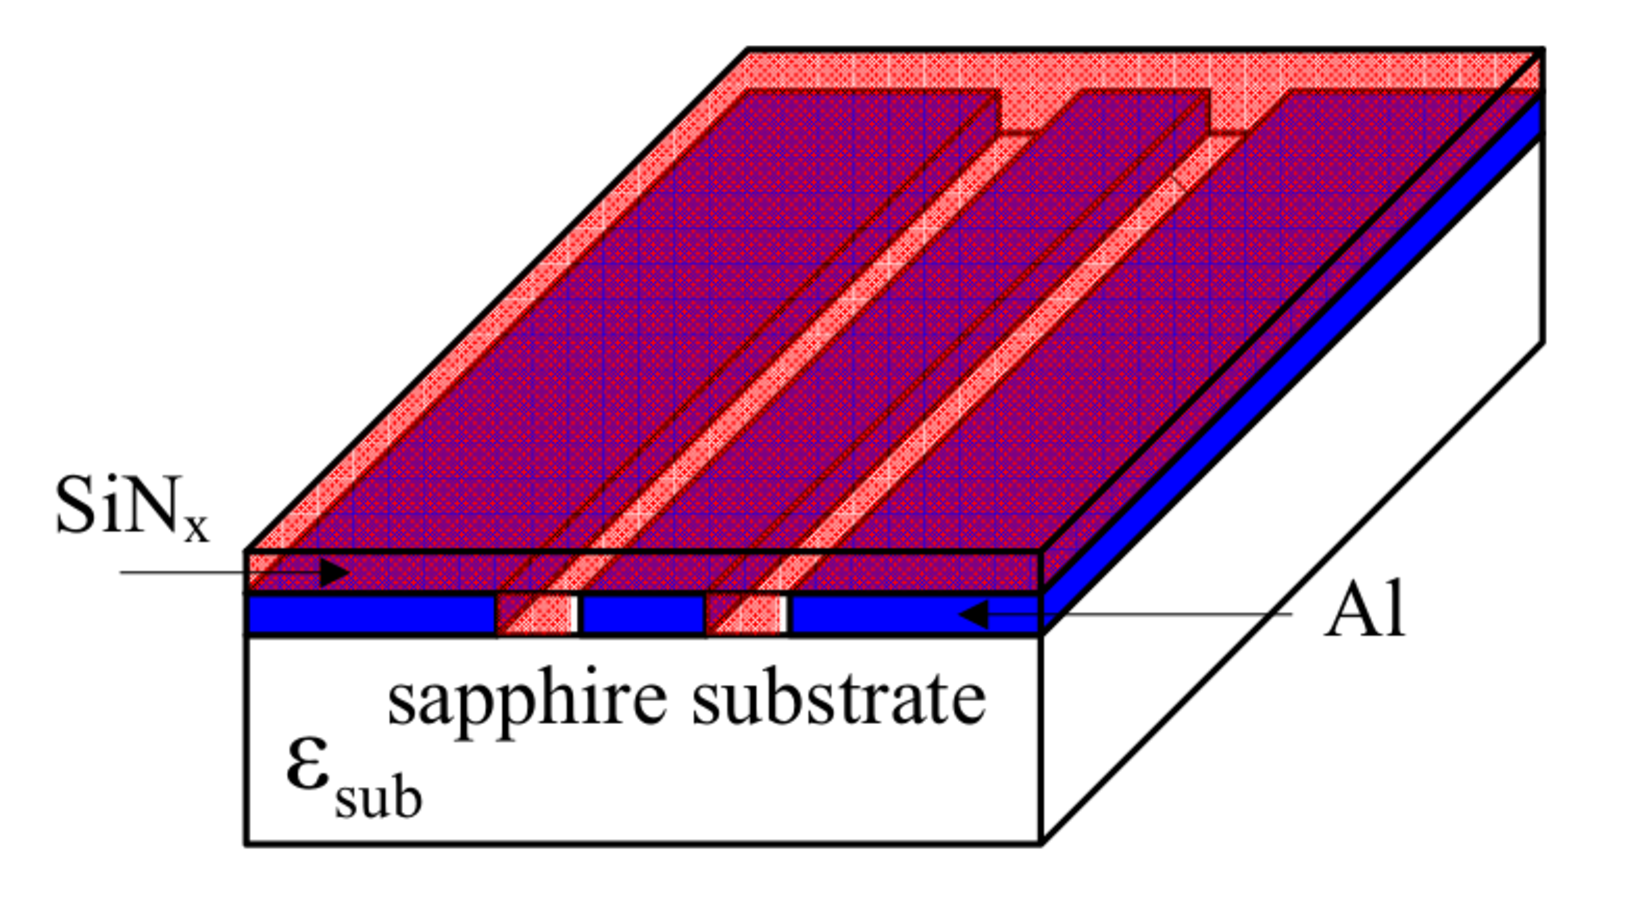
\includegraphics[height=0.5\textheight,width=0.9\textwidth]{nitruro_de_silicio_mkid}}
				\end{center}
				\only<3>{\tiny{Pulso de respuesta de un
				resonador CPW  de \alert{$Al/Al_2 O_3$}
				que indica la detección de fotones de rayos X de
				$5.9\,\text{keV}$ ({\color[rgb]{0.1,0.1,0.9} Day PK, Leduc HG, Mazin BA, Vayonakis
				A, Zmuidzinas J. 2003. Nature 425:817–21})}}
\end{column}
\end{columns}
\end{frame} 

%------------------------------------------------------------------------------
\section{Conclusiones}
%------------------------------------------------------------------------------
\begin{frame}
\frametitle{Conclusiones}
%\begin{block}{}
\begin{itemize}
\item[$\triangleright$] Vimos los principales factores de calidad que deben
				tener los	detectores superconductores para ser usados en la detección de
								partículas/radiación.
\item[$\triangleright$] En general, podemos dividir a los detectores de
				partículas superconductores como bolómetros o detectores térmicos y
								detectores de no equilibrio (procesos hot electron) 
\item[$\triangleright$] Analizamos el funcionamiento de un nuevo tipo de
				detectores superconductores, los MKIDs
\item[$\triangleright$] \alert{Los superconductores vienen siendo la tecnología más
				prometedora para los próximos descubrimientos en astropartículas}
\end{itemize}
%\end{block}
\end{frame} 


\begin{frame}
				\begin{center}
								%\huge{¡Muchas Gracias!}
								
\includegraphics[height=0.6\textheight,width=0.65\textwidth]{logos/gracias}
				\end{center}
\end{frame}

%\begin{frame}
%				\begin{center}
%								\huge{¿Preguntas?}\\
%								\vspace{5mm}
%								
\includegraphics[height=0.4\textheight,width=0.4\textwidth]{logos/preguntas}
%				\end{center}
%\end{frame}


\end{document}
